\documentclass[11pt,a4paper]{article}

% ==================== TEMEL PAKETLER (pdflatex) ====================
\usepackage[T1]{fontenc}
\usepackage[utf8]{inputenc}
\usepackage{lmodern}
\usepackage[a4paper,margin=2cm,top=2.4cm,bottom=2.4cm]{geometry}
\usepackage{xcolor}
\usepackage{colortbl}
\usepackage{array}
\usepackage{booktabs}
\usepackage{longtable}
\usepackage{tabularx}
\usepackage{listings}
\usepackage{amsmath}
\usepackage{amssymb}
\usepackage{fancyhdr}
\usepackage{tikz}
\usetikzlibrary{arrows.meta,calc,patterns}
\usepackage{hyperref}

% ==================== RENK PALETİ ====================
\definecolor{anaMavi}{HTML}{1B3A5B}
\definecolor{vurguMavi}{HTML}{2E6DA4}
\definecolor{acikMavi}{HTML}{EAF2F9}
\definecolor{turuncu}{HTML}{D9701E}
\definecolor{yesil}{HTML}{2E7D32}
\definecolor{acikYesil}{HTML}{E8F5E9}
\definecolor{kirmizi}{HTML}{C0392B}
\definecolor{mor}{HTML}{6C3483}
\definecolor{acikMor}{HTML}{F3E9F7}
\definecolor{acikGri}{HTML}{F4F5F7}
\definecolor{ortaGri}{HTML}{6B7280}
\definecolor{koyuGri}{HTML}{2D2D2D}
\definecolor{grafikMavi}{HTML}{2E6DA4}
\definecolor{kodArka}{HTML}{FBFBFA}

% ==================== HYPERREF ====================
\hypersetup{
  colorlinks=true,
  linkcolor={[HTML]{2E6DA4}},
  urlcolor={[HTML]{2E6DA4}},
  pdftitle={Python ile Kalkülüs 1 ve Kalkülüs 2 Rehberi},
  pdfauthor={Kalkülüs Rehberi},
  bookmarksnumbered=true
}

% ==================== BAŞLIK STİLLERİ ====================
\setcounter{secnumdepth}{0}
\newcounter{secc}
\newcounter{subsecc}[secc]
\newcounter{subsubsecc}[subsecc]
\newcommand{\gsec}[1]{\par\phantomsection\stepcounter{secc}%
  \setcounter{subsecc}{0}%
  \vspace{18pt}{\color{anaMavi}\Large\bfseries\thesecc.\hspace{0.5em}#1}\par
  \vspace{2pt}{\color{turuncu}\rule{\linewidth}{1.6pt}}\par\vspace{8pt}%
  \addcontentsline{toc}{section}{\protect\numberline{\thesecc}#1}\markboth{#1}{#1}}
\newcommand{\gsub}[1]{\par\phantomsection\stepcounter{subsecc}%
  \setcounter{subsubsecc}{0}%
  \vspace{11pt}{\color{vurguMavi}\large\bfseries\thesecc.\thesubsecc\hspace{0.5em}#1}\par\vspace{4pt}%
  \addcontentsline{toc}{subsection}{\protect\numberline{\thesecc.\thesubsecc}#1}}
\newcommand{\gsubsub}[1]{\par\vspace{7pt}{\color{koyuGri}\normalsize\bfseries #1}\par\vspace{2pt}}

% Kısım (Part) başlığı
\newcommand{\gpart}[2]{\clearpage
  \begin{center}\vspace*{1.5cm}
  {\color{turuncu}\rule{0.7\linewidth}{1.5pt}}\\[10pt]
  {\color{ortaGri}\Large KISIM #1}\\[8pt]
  {\color{anaMavi}\Huge\bfseries #2}\\[10pt]
  {\color{turuncu}\rule{0.7\linewidth}{1.5pt}}
  \end{center}\vspace{1cm}}

% ==================== BAŞLIK / ALTBİLGİ ====================
\setlength{\headheight}{14pt}
\pagestyle{fancy}
\fancyhf{}
\renewcommand{\headrulewidth}{0.4pt}
\renewcommand{\footrulewidth}{0.4pt}
\fancyhead[L]{\small\color{ortaGri}Python ile Kalkülüs 1--2}
\fancyhead[R]{\small\color{ortaGri}\leftmark}
\fancyfoot[C]{\small\color{ortaGri}\thepage}

% ==================== KOD LİSTELEME (Python) ====================
\lstdefinestyle{pystyle}{
  language=Python,
  basicstyle=\ttfamily\small\color{koyuGri},
  keywordstyle=\color{vurguMavi}\bfseries,
  commentstyle=\color{yesil}\itshape,
  stringstyle=\color{turuncu},
  numberstyle=\tiny\color{ortaGri},
  numbers=left,
  numbersep=8pt,
  backgroundcolor=\color{kodArka},
  frame=single,
  framesep=6pt,
  rulecolor=\color{ortaGri!40},
  breaklines=true,
  showstringspaces=false,
  tabsize=4,
  columns=fullflexible,
  keepspaces=true,
  extendedchars=true,
  literate={ı}{{\i}}1{İ}{{\.I}}1{ş}{{\c s}}1{Ş}{{\c S}}1{ğ}{{\u g}}1{Ğ}{{\u G}}1{ç}{{\c c}}1{Ç}{{\c C}}1{ö}{{\"o}}1{Ö}{{\"O}}1{ü}{{\"u}}1{Ü}{{\"U}}1,
  morekeywords={sp,np,plt,sym,as,with,yield,lambda,None,True,False,self,
    assert,symbols,diff,integrate,limit,solve,simplify,expand,factor,
    series,summation,lambdify,Rational,oo,pi,sqrt,sin,cos,tan,exp,log,
    linspace,array,quad,dsolve,solve_ivp,Function,Eq,plot,subs,evalf}
}
\lstset{style=pystyle}

% Kabuk/terminal stili
\lstdefinestyle{shstyle}{
  numbers=none,
  basicstyle=\ttfamily\small\color{koyuGri},
  backgroundcolor=\color{koyuGri!6},
  frame=single,framesep=6pt,rulecolor=\color{ortaGri!40},
  breaklines=true,showstringspaces=false,tabsize=4,columns=fullflexible,
  keepspaces=true,
  literate={ı}{{\i}}1{İ}{{\.I}}1{ş}{{\c s}}1{Ş}{{\c S}}1{ğ}{{\u g}}1{Ğ}{{\u G}}1{ç}{{\c c}}1{Ç}{{\c C}}1{ö}{{\"o}}1{Ö}{{\"O}}1{ü}{{\"u}}1{Ü}{{\"U}}1,
}

% Program çıktısı stili
\lstdefinestyle{outstyle}{
  numbers=none,
  basicstyle=\ttfamily\small\color{anaMavi},
  backgroundcolor=\color{acikMavi},
  frame=single,framesep=6pt,rulecolor=\color{vurguMavi!40},
  breaklines=true,showstringspaces=false,tabsize=4,columns=fullflexible,
  keepspaces=true,
  literate={ı}{{\i}}1{İ}{{\.I}}1{ş}{{\c s}}1{Ş}{{\c S}}1{ğ}{{\u g}}1{Ğ}{{\u G}}1{ç}{{\c c}}1{Ç}{{\c C}}1{ö}{{\"o}}1{Ö}{{\"O}}1{ü}{{\"u}}1{Ü}{{\"U}}1,
}

% ==================== ÖZEL KUTULAR ====================
\newcommand{\callout}[4]{\par\smallskip\noindent\begingroup
  \setlength{\fboxsep}{8pt}\setlength{\fboxrule}{0.8pt}%
  \fcolorbox{#1}{#2}{\parbox{\dimexpr\linewidth-2\fboxsep-2\fboxrule\relax}{%
    {\bfseries\color{#1}#3}\par\smallskip #4}}\endgroup\par\smallskip}
\newcommand{\bilgi}[1]{\callout{vurguMavi}{acikMavi}{Bilgi}{#1}}
\newcommand{\ipucu}[1]{\callout{yesil}{acikYesil}{İpucu}{#1}}
\newcommand{\uyari}[1]{\callout{kirmizi}{kirmizi!7}{Dikkat}{#1}}
\newcommand{\tanim}[2][Tanım]{\callout{vurguMavi}{acikMavi}{#1}{#2}}
\newcommand{\kural}[2][Kural]{\callout{mor}{acikMor}{#1}{#2}}
\newcommand{\teorem}[2][Teorem]{\callout{mor}{acikMor}{#1}{#2}}
\newcommand{\notk}[2][Not]{\callout{mor}{acikMor}{#1}{#2}}
\newcommand{\ornek}[2][Örnek]{\callout{ortaGri!90!black}{acikGri}{#1}{#2}}

% Soru / Çözüm sistemi
\newcounter{soruc}
\newcommand{\soru}[1]{\par\smallskip\refstepcounter{soruc}%
  \noindent\begingroup\setlength{\fboxsep}{8pt}\setlength{\fboxrule}{0.8pt}%
  \fcolorbox{turuncu}{turuncu!6}{\parbox{\dimexpr\linewidth-2\fboxsep-2\fboxrule\relax}{%
  {\bfseries\color{turuncu}Soru \thesoruc}\par\smallskip #1}}\endgroup\par\smallskip}
\newcommand{\cozum}{\par\noindent{\bfseries\color{yesil}Çözüm.}\ }
\newcommand{\pykontrol}{\par\noindent{\bfseries\color{vurguMavi}Python ile kontrol.}\ }

% Yardımcı komutlar
\newcommand{\code}[1]{\texttt{\color{koyuGri}#1}}
\renewcommand{\arraystretch}{1.35}
\newcommand{\lm}[2]{\lim_{#1 \to #2}}
\newcommand{\dd}{\,\mathrm{d}}

% ==================== BAŞLANGIÇ ====================
\begin{document}

% ---------- KAPAK ----------
\begin{titlepage}
\centering
\vspace*{0.5cm}
{\color{turuncu}\rule{\textwidth}{2pt}}\\[8pt]
{\color{anaMavi}\Huge\bfseries Python ile Kalkülüs}\\[10pt]
{\color{vurguMavi}\LARGE Calculus 1 ve Calculus 2 --- Tam Konu Rehberi}\\[8pt]
{\color{ortaGri}\large SymPy \textbullet\ NumPy \textbullet\ SciPy \textbullet\ Matplotlib}\\[6pt]
{\color{turuncu}\rule{\textwidth}{2pt}}\\[0.8cm]

\begin{center}
\fcolorbox{vurguMavi}{acikMavi}{\parbox{0.86\textwidth}{\centering\large
Bu belge, üniversite \textbf{Calculus 1} ve \textbf{Calculus 2} müfredatının
tamamını sıfırdan anlatır. Her konu önce \textbf{sezgisel} olarak, sonra
\textbf{tanım ve teoremleriyle} verilir; ardından elle çözülen sorularla
pekiştirilir ve aynı sonuç \textbf{Python (SymPy/NumPy/SciPy)} ile
doğrulanır.\vspace{4pt}}}
\end{center}

\vspace{0.5cm}
\begin{center}
\fcolorbox{ortaGri!50}{acikGri}{\parbox{0.86\textwidth}{\footnotesize
\textbf{Kısım 1 --- Python Araç Kutusu:} kurulum \textbullet\ SymPy sembolik
matematik \textbullet\ NumPy sayısal hesap \textbullet\ Matplotlib ile grafik
\textbullet\ \code{lambdify} köprüsü.\vspace{4pt}

\textbf{Kısım 2 --- Calculus 1 / Limit:} fonksiyonlar \textbullet\ limit kavramı
\textbullet\ tek taraflı limitler \textbullet\ limit teknikleri \textbullet\
sıkıştırma teoremi \textbullet\ $\varepsilon$-$\delta$ kesin tanım
\textbullet\ süreklilik \textbullet\ ara değer teoremi \textbullet\ sonsuz
limitler \textbullet\ sonsuzda limit \& asimptotlar.\vspace{4pt}

\textbf{Kısım 3 --- Calculus 1 / Türev:} tanım \& teğet \textbullet\ türev
kuralları \textbullet\ zincir kuralı \textbullet\ kapalı ve logaritmik türev
\textbullet\ ilişkili değişim oranları \textbullet\ lineerleştirme \& Newton
\textbullet\ ters \& hiperbolik fonksiyonların türevi \textbullet\ doğrusal
hareket \& marjinal analiz \textbullet\ MVT \textbullet\ ekstremum, konkavlık,
eğri çizimi \textbullet\ optimizasyon \textbullet\ L'Hôpital.\vspace{4pt}

\textbf{Kısım 4 --- Calculus 1 / İntegrale Giriş:} ters türev \textbullet\
Riemann toplamları \textbullet\ belirli integral \textbullet\ Kalkülüsün Temel
Teoremi \textbullet\ yerine koyma \textbullet\ başlangıç koşullu problemler
\textbullet\ ortalama değer.\vspace{4pt}

\textbf{Kısım 5 --- Calculus 2 / İntegral Teknikleri:} kısmi integral
\textbullet\ trigonometrik integraller \& yerine koyma \textbullet\ kısmi
kesirler \textbullet\ sayısal integral \textbullet\ genelleştirilmiş
integraller.\vspace{4pt}

\textbf{Kısım 6 --- Calculus 2 / Uygulamalar:} alan \textbullet\ disk, halka ve
silindirik kabuk hacimleri \textbullet\ yay uzunluğu \textbullet\ dönel yüzey
alanı \textbullet\ iş \textbullet\ kütle merkezi \textbullet\ olasılık
\textbullet\ ekonomi \& biyoloji uygulamaları.\vspace{4pt}

\textbf{Kısım 7 --- Calculus 2 / Diferansiyel Denklemler:} yön alanları
\textbullet\ ayrılabilir denklemler \textbullet\ birinci mertebe lineer
\textbullet\ Euler yöntemi \textbullet\ lojistik büyüme \textbullet\ karışım
problemleri \textbullet\ ortogonal yörüngeler \textbullet\ av-avcı
sistemleri.\vspace{4pt}

\textbf{Kısım 8 --- Calculus 2 / Diziler ve Seriler:} diziler \textbullet\
geometrik \& teleskopik seriler \textbullet\ integral, karşılaştırma, oran ve
kök testleri \textbullet\ alterne seriler \textbullet\ mutlak yakınsaklık
\textbullet\ kalan tahmini.\vspace{4pt}

\textbf{Kısım 9 --- Calculus 2 / Kuvvet Serileri:} yakınsaklık yarıçapı
\textbullet\ Taylor \& Maclaurin serileri \textbullet\ hata (kalan) tahmini
\textbullet\ binom serisi \textbullet\ seri uygulamaları.\vspace{4pt}

\textbf{Kısım 10 --- Calculus 2 / Parametrik ve Kutupsal:} parametrik eğriler
\textbullet\ parametrik türev \& yay uzunluğu \textbullet\ kutupsal koordinatlar
\textbullet\ kutupsal alan \textbullet\ simetri \& kesişim \textbullet\
konikler (parabol, elips, hiperbol) \textbullet\ koniklerin kutupsal
biçimi.\vspace{4pt}

\textbf{Kısım 11 --- Referans:} tüm formüller \textbullet\ SymPy/SciPy
fonksiyon sözlüğü \textbullet\ hızlı tarif kitabı.\vspace{4pt}}}
\end{center}

\vfill
{\color{ortaGri}\large Hazırlanma Tarihi: 9 Eylül 2026}\\[4pt]
{\color{ortaGri} Terimler İngilizce \textbullet\ Anlatım Türkçe \textbullet\ Kod Python 3}
\vspace*{0.4cm}
\end{titlepage}

% ---------- İÇİNDEKİLER ----------
\tableofcontents
\thispagestyle{empty}
\clearpage

% #####################################################################
\gpart{1}{Python Araç Kutusu}
% #####################################################################

% =====================================================================
\gsec{Neden Kalkülüsü Python ile Öğrenmeli?}
% =====================================================================

Kalkülüs, \emph{değişimi} ve \emph{birikimi} inceleyen matematiktir. Limit,
türev ve integral kavramları kâğıt üzerinde sembolik olarak öğrenilir; ancak
bu kavramların hepsi aynı zamanda \emph{sayısal} ve \emph{görsel} nesnelerdir.
Python, üç şeyi aynı anda yapabildiği için kalkülüs öğrenirken güçlü bir
laboratuvardır:

\begin{itemize}\itemsep2pt
\item \textbf{Sembolik hesap (SymPy):} Türev ve integrali tıpkı elle yaptığın
gibi \emph{formül} olarak alır. Çözümünü saniyeler içinde doğrularsın.
\item \textbf{Sayısal hesap (NumPy/SciPy):} Limitin tanımındaki ``yaklaşma''yı
tablo hâlinde görürsün; Riemann toplamını gerçekten hesaplarsın.
\item \textbf{Görselleştirme (Matplotlib):} Teğet doğruyu, eğri altındaki
alanı, yakınsayan seriyi gözünle görürsün.
\end{itemize}

\uyari{Python bir \emph{doğrulama} ve \emph{sezgi} aracıdır, çözümün yerine
geçmez. Sınavda \code{sp.integrate} yazamazsın. Bu rehberdeki her soruyu önce
elle çöz, sonra kodla kontrol et. ``Kod doğru sonucu verdi'' demek ``konuyu
anladım'' demek değildir.}

\gsub{Kurulum}

\begin{lstlisting}[style=shstyle]
# Sanal ortam (izole, temiz kurulum)
$ python3 -m venv kalkulus
$ source kalkulus/bin/activate        # Linux / macOS
# kalkulus\Scripts\activate           # Windows

# Gerekli kutuphaneler
$ pip install sympy numpy scipy matplotlib

# Interaktif calisma icin (onerilir)
$ pip install jupyter
$ jupyter notebook
\end{lstlisting}

\gsub{Kütüphanelerin Rolleri}

\begin{center}
\begin{tabularx}{\textwidth}{@{}>{\ttfamily\bfseries\color{anaMavi}}l X@{}}
\toprule
\rowcolor{acikMavi}\multicolumn{1}{@{}l}{\color{anaMavi}\textbf{Kütüphane}} & \multicolumn{1}{l@{}}{\color{anaMavi}\textbf{Kalkülüsteki rolü}}\\
\midrule
SymPy & Sembolik matematik: limit, türev, integral, seri, denklem çözme. Kâğıt üzerindeki cebirin karşılığı.\\
\rowcolor{acikGri} NumPy & Sayı dizileri: fonksiyonu binlerce noktada hızlıca hesaplama, Riemann toplamı, vektörleştirme.\\
Matplotlib & Grafik: fonksiyon, teğet, alan, yön alanı, yakınsaklık grafikleri.\\
\rowcolor{acikGri} SciPy & Sayısal analiz: \code{quad} (integral), \code{solve\_ivp} (diferansiyel denklem), \code{minimize} (optimizasyon), kök bulma.\\
\bottomrule
\end{tabularx}
\end{center}

% =====================================================================
\gsec{SymPy Temelleri}
% =====================================================================

SymPy'de her şey \emph{sembol} ile başlar. Normal Python'da \code{x} bir
değişkendir ve bir değer tutar; SymPy'de \code{x} bir \emph{matematiksel
belirsiz}dir ve değer tutmaz.

\gsub{Sembol Tanımlama ve İfadeler}

\begin{lstlisting}
import sympy as sp

# Sembol tanimla
x, y, t = sp.symbols('x y t')            # gercek/karmasik olabilir
n = sp.symbols('n', integer=True, positive=True)
a, b = sp.symbols('a b', real=True)

# Ifade kur (otomatik sadelesme yapilir, tam yapilmaz)
f = x**2 + 3*x + 2
print(f)                                  # x**2 + 3*x + 2

# Guzel gorunum (konsolda ASCII matematik)
sp.init_printing(use_unicode=True)
sp.pprint(f)
\end{lstlisting}

\uyari{\code{x = sp.symbols('x')} satırını unutursan \code{NameError} alırsın.
Ayrıca \code{sp.symbols('x')} ile \code{sp.Symbol('x')} aynı nesneyi üretir;
çoklu tanım için \code{symbols} pratiktir.}

\gsub{Sadeleştirme, Açma, Çarpanlara Ayırma}

\begin{lstlisting}
expr = (x**2 - 1)/(x - 1)

sp.simplify(expr)          # x + 1        -> genel amacli sadelestirme
sp.expand((x + 2)**3)      # x**3 + 6*x**2 + 12*x + 8
sp.factor(x**3 - x)        # x*(x - 1)*(x + 1)
sp.cancel((x**2 - 1)/(x**2 + 2*x + 1))    # (x - 1)/(x + 1)
sp.apart(1/(x**2 - 1))     # kismi kesirlere ayirir
sp.together(1/x + 1/y)     # tek kesirde toplar
sp.trigsimp(sp.sin(x)**2 + sp.cos(x)**2)  # 1
\end{lstlisting}

\begin{center}
\begin{tabularx}{\textwidth}{@{}>{\ttfamily\color{anaMavi}}l X@{}}
\toprule
\rowcolor{acikMavi}\multicolumn{1}{@{}l}{\color{anaMavi}\textbf{Fonksiyon}} & \multicolumn{1}{l@{}}{\color{anaMavi}\textbf{Ne yapar?}}\\
\midrule
simplify(e) & Genel sadeleştirme; ne yapacağını kendisi seçer (yavaş olabilir).\\
\rowcolor{acikGri} expand(e) & Parantezleri açar, çarpımları dağıtır.\\
factor(e) & Polinomu çarpanlara ayırır.\\
\rowcolor{acikGri} cancel(e) & Rasyonel ifadede ortak çarpanları sadeleştirir.\\
apart(e) & Kısmi kesirlere ayırır (integral için kritik).\\
\rowcolor{acikGri} together(e) & Kesirleri ortak paydada birleştirir.\\
trigsimp(e) & Trigonometrik özdeşliklerle sadeleştirir.\\
\rowcolor{acikGri} radsimp(e) & Paydadaki kökleri rasyonelleştirir (eşlenikle çarpar).\\
\bottomrule
\end{tabularx}
\end{center}

\gsub{Değer Yerine Koyma ve Sayısal Değer}

\begin{lstlisting}
f = x**2 + 3*x + 2

f.subs(x, 2)                 # 12         -> tam (exact) sonuc
f.subs(x, sp.Rational(1,2))  # 15/4       -> kesir olarak kalir
f.subs(x, 0.5)               # 3.75

# Cok degiskenli yerine koyma
g = x*y + y**2
g.subs({x: 1, y: 2})         # 6

# Ondalik degere cevirme
sp.sqrt(2).evalf()           # 1.41421356237310
sp.pi.evalf(30)              # 30 basamak
float(sp.sqrt(2))            # normal Python float
\end{lstlisting}

\uyari{SymPy'de \code{1/3} yazarsan Python bunu \code{0.3333...} float'ına
çevirir ve kesinlik kaybedersin. Tam kesir için \code{sp.Rational(1,3)} veya
\code{sp.S(1)/3} kullan.}

\gsub{Denklem Çözme}

\begin{lstlisting}
# Denklem: sag taraf 0 kabul edilir ya da Eq ile yazilir
sp.solve(x**2 - 4, x)                  # [-2, 2]
sp.solve(sp.Eq(x**2, 4), x)            # [-2, 2]

# Sistem
sp.solve([x + y - 3, x - y - 1], [x, y])   # {x: 2, y: 1}

# Cozum kumesi (daha guclu, sonsuz cozumleri de verir)
sp.solveset(sp.sin(x), x, domain=sp.S.Reals)   # {2*n*pi} U {2*n*pi + pi}

# Sayisal kok (baslangic tahminiyle)
sp.nsolve(sp.cos(x) - x, x, 1)         # 0.739085133215161
\end{lstlisting}

\gsub{Kalkülüs Komutları: Dört Temel Fonksiyon}

Bütün rehber boyunca dönüp dolaşıp aşağıdaki dört komutu kullanacağız.

\begin{center}
\begin{tabularx}{\textwidth}{@{}>{\ttfamily\color{anaMavi}}l X@{}}
\toprule
\rowcolor{acikMavi}\multicolumn{1}{@{}l}{\color{anaMavi}\textbf{Komut}} & \multicolumn{1}{l@{}}{\color{anaMavi}\textbf{Anlamı}}\\
\midrule
sp.limit(f, x, a) & $\lim_{x\to a} f(x)$. Yön için \code{dir='+'} veya \code{dir='-'}.\\
\rowcolor{acikGri} sp.diff(f, x) & $f'(x)$. \code{sp.diff(f, x, 2)} ikinci türev.\\
sp.integrate(f, x) & Belirsiz integral $\int f\dd x$ (sabit $C$ eklenmez).\\
\rowcolor{acikGri} sp.integrate(f, (x,a,b)) & Belirli integral $\int_a^b f\dd x$.\\
sp.series(f, x, a, n) & $f$'nin $a$ etrafında $n$. mertebeden Taylor açılımı.\\
\rowcolor{acikGri} sp.summation(a, (n,1,oo)) & $\sum_{n=1}^{\infty} a_n$ serisinin toplamı.\\
\bottomrule
\end{tabularx}
\end{center}

\begin{lstlisting}
import sympy as sp
x = sp.symbols('x')

sp.limit(sp.sin(x)/x, x, 0)          # 1
sp.diff(x**3 * sp.exp(x), x)         # x**3*exp(x) + 3*x**2*exp(x)
sp.integrate(sp.log(x), x)           # x*log(x) - x
sp.integrate(sp.exp(-x**2), (x, -sp.oo, sp.oo))   # sqrt(pi)
sp.series(sp.cos(x), x, 0, 8)        # 1 - x**2/2 + x**4/24 - x**6/720 + O(x**8)
sp.summation(1/sp.Symbol('n', positive=True)**2, ('n', 1, sp.oo))  # pi**2/6
\end{lstlisting}

\bilgi{Sonsuz sembolü SymPy'de \code{sp.oo} (iki küçük harf o) ile yazılır.
Negatif sonsuz \code{-sp.oo}, tanımsız \code{sp.nan}, sanal birim \code{sp.I},
$e$ sayısı \code{sp.E}, $\pi$ ise \code{sp.pi}'dir.}

% =====================================================================
\gsec{NumPy, Matplotlib ve İkisi Arasındaki Köprü}
% =====================================================================

SymPy formülle, NumPy sayılarla çalışır. Bir SymPy ifadesini binlerce noktada
hesaplamak (yani \emph{grafiğini çizmek}) istiyorsak, onu hızlı bir NumPy
fonksiyonuna çevirmemiz gerekir: bunu \code{sp.lambdify} yapar.

\gsub{lambdify: Sembolden Sayıya}

\begin{lstlisting}
import numpy as np
import sympy as sp
import matplotlib.pyplot as plt

x = sp.symbols('x')
f = sp.sin(x)/x                       # sembolik ifade

f_num = sp.lambdify(x, f, 'numpy')    # hizli NumPy fonksiyonu

xs = np.linspace(-10, 10, 1000)
ys = f_num(xs)                        # 1000 noktada tek seferde hesap

plt.plot(xs, ys, color='#2E6DA4', lw=2)
plt.axhline(0, color='gray', lw=0.8)
plt.axvline(0, color='gray', lw=0.8)
plt.grid(alpha=0.3)
plt.title(r'$f(x) = \frac{\sin x}{x}$')
plt.show()
\end{lstlisting}

\ipucu{Matplotlib başlıklarında \code{r'\$...\$'} yazarak LaTeX matematiği
kullanabilirsin: \code{r'\$\textbackslash int\_0\^{}1 x\^{}2\textbackslash,dx\$'}
gibi. Başındaki \code{r} (raw string) ters bölü karakterlerinin bozulmamasını
sağlar.}

\gsub{Standart Grafik Şablonu}

Rehber boyunca kullanacağımız, eksenleri ortadan geçen ``matematik kitabı''
görünümlü şablon:

\begin{lstlisting}
import numpy as np
import matplotlib.pyplot as plt

def eksen_kur(xlim=(-5, 5), ylim=(-5, 5), baslik=''):
    """Eksenleri ortadan gecen temiz bir grafik kurar."""
    fig, ax = plt.subplots(figsize=(6, 4.5))
    ax.spines['left'].set_position('zero')
    ax.spines['bottom'].set_position('zero')
    ax.spines['right'].set_visible(False)
    ax.spines['top'].set_visible(False)
    ax.set_xlim(*xlim); ax.set_ylim(*ylim)
    ax.grid(alpha=0.25)
    ax.set_title(baslik)
    return fig, ax

fig, ax = eksen_kur((-3, 3), (-1, 9), r'$f(x)=x^2$')
xs = np.linspace(-3, 3, 400)
ax.plot(xs, xs**2, color='#2E6DA4', lw=2)
plt.show()
\end{lstlisting}

\gsub{Sık Kullanılan NumPy Araçları}

\begin{center}
\begin{tabularx}{\textwidth}{@{}>{\ttfamily\color{anaMavi}}l X@{}}
\toprule
\rowcolor{acikMavi}\multicolumn{1}{@{}l}{\color{anaMavi}\textbf{Komut}} & \multicolumn{1}{l@{}}{\color{anaMavi}\textbf{Ne işe yarar?}}\\
\midrule
np.linspace(a,b,n) & $[a,b]$ aralığını $n$ eşit noktaya böler (uç noktalar dâhil).\\
\rowcolor{acikGri} np.arange(a,b,h) & $a$'dan $b$'ye $h$ adımlarla (uç hariç).\\
np.sum(v) & Dizinin toplamı --- Riemann toplamının kalbi.\\
\rowcolor{acikGri} np.cumsum(v) & Kümülatif toplam --- kısmi toplam dizisi.\\
np.diff(v) & Ardışık farklar --- sayısal türevin payı.\\
\rowcolor{acikGri} np.gradient(y,x) & Merkezî farkla sayısal türev.\\
np.trapz(y,x) & Yamuk kuralıyla sayısal integral.\\
\rowcolor{acikGri} np.abs, np.max & Mutlak değer, maksimum (hata analizi için).\\
\bottomrule
\end{tabularx}
\end{center}

\ipucu{Bu rehberdeki her kod parçası kendi başına çalışacak şekilde yazılmıştır;
ancak yer kazanmak için \code{import} satırları çoğu zaman tekrarlanmaz. Bir
Jupyter oturumunda en başta şunları çalıştır:\\
\code{import sympy as sp; import numpy as np; import matplotlib.pyplot as plt}\\
\code{x, y, t, n = sp.symbols('x y t n')}}

% #####################################################################
\gpart{2}{Calculus 1 --- Fonksiyonlar, Limit ve Süreklilik}
% #####################################################################

% =====================================================================
\gsec{Fonksiyonlar: Kısa Ama Gerekli Tekrar}
% =====================================================================

Kalkülüs, fonksiyonlar üzerinde yapılan bir hesaptır. Limit, türev ve integral
almadan önce hangi fonksiyonla uğraştığımızı tanımak zorundayız.

\gsub{Tanım Kümesi ve Görüntü Kümesi}

\tanim{Bir $f$ fonksiyonu, tanım kümesindeki (domain) her $x$ değerine tam bir
$f(x)$ değeri eşleyen kuraldır. Alabildiği tüm $f(x)$ değerlerinin kümesine
görüntü kümesi (range) denir.}

Tanım kümesini bulurken üç yasak vardır: \textbf{sıfıra bölme}, \textbf{negatif
sayının çift dereceli kökü} ve \textbf{sıfır veya negatifin logaritması}.

\ornek{$f(x)=\dfrac{\sqrt{x-1}}{x-3}$ fonksiyonunun tanım kümesi: kök içi
$x-1\ge 0 \Rightarrow x\ge 1$; payda $x-3\neq 0 \Rightarrow x\neq 3$. Sonuç:
$[1,3)\cup(3,\infty)$.}

\begin{lstlisting}
import sympy as sp
x = sp.symbols('x', real=True)

f = sp.sqrt(x - 1)/(x - 3)
sp.calculus.util.continuous_domain(f, x, sp.S.Reals)
# Union(Interval.Ropen(1, 3), Interval.open(3, oo))

# Goruntu kumesi (basit fonksiyonlar icin)
sp.calculus.util.function_range(x**2, x, sp.S.Reals)   # Interval(0, oo)
\end{lstlisting}

\gsub{Temel Fonksiyon Aileleri}

\begin{center}
\renewcommand{\arraystretch}{2.4}
\begin{tabularx}{\textwidth}{@{}>{\bfseries\color{anaMavi}}l >{$}l<{$} X@{}}
\toprule
\rowcolor{acikMavi}\multicolumn{1}{@{}l}{\color{anaMavi}\textbf{Aile}} & \multicolumn{1}{l}{\color{anaMavi}\textbf{Biçim}} & \multicolumn{1}{l@{}}{\color{anaMavi}\textbf{Temel özellik}}\\
\midrule
Polinom & a_nx^n+\dots+a_0 & Her yerde sürekli ve türevlenebilir.\\
\rowcolor{acikGri} Rasyonel & P(x)/Q(x) & $Q(x)=0$ noktalarında tanımsız; düşey asimptot.\\
Kök & \sqrt[n]{x} & Çift $n$ için $x\ge 0$.\\
\rowcolor{acikGri} Üstel & a^x,\ e^x & Hep pozitif; $e^x$ türevi kendisi.\\
Logaritmik & \log_a x,\ \ln x & Yalnız $x>0$; üstelin tersi.\\
\rowcolor{acikGri} Trigonometrik & \sin x,\cos x,\tan x & Periyodik; $\tan$'ın düşey asimptotları var.\\
Ters trigonometrik & \arcsin x,\arctan x & Sınırlı tanım/görüntü kümesi.\\
\rowcolor{acikGri} Parçalı & \text{koşullu} & Ek noktalarında süreklilik ayrı kontrol edilir.\\
\bottomrule
\end{tabularx}
\end{center}

\begin{lstlisting}
# Parcali fonksiyon: f(x) = x^2 (x<1),  2x (x>=1)
f = sp.Piecewise((x**2, x < 1), (2*x, True))
f.subs(x, 0.5)     # 0.25
f.subs(x, 3)       # 6
sp.diff(f, x)      # parcali turev
\end{lstlisting}

\gsub{Bileşke ve Ters Fonksiyon}

$(f\circ g)(x)=f(g(x))$ bileşkedir; zincir kuralının konusudur. $f^{-1}$ ters
fonksiyondur ve $f(f^{-1}(x))=x$ sağlanır.

\begin{lstlisting}
f = x**2 + 1
g = sp.sin(x)

bileske = f.subs(x, g)          # sin(x)**2 + 1
y = sp.symbols('y')
sp.solve(sp.Eq(y, 2*x + 3), x)  # [y/2 - 3/2]  -> ters fonksiyon
\end{lstlisting}

% =====================================================================
\gsec{Limit Kavramı}
% =====================================================================

Limit, kalkülüsün temel taşıdır; hem türev hem integral limit üzerine
kuruludur. Sezgisel olarak limit şu soruyu sorar: ``$x$ bir $a$ değerine
\emph{yaklaşırken}, $f(x)$ hangi değere \emph{yaklaşır}?'' Dikkat: soru
``$f(a)$ nedir?'' değildir --- limit, fonksiyonun o noktadaki değeriyle değil,
\emph{yakınındaki} davranışıyla ilgilenir.

\gsub{Sezgisel Tanım ve Gösterim}

\tanim{$x$, $a$'ya yaklaşırken $f(x)$ değeri $L$ sayısına istenildiği kadar
yaklaşıyorsa, $f$'nin $a$ noktasındaki \emph{limiti} $L$'dir:
\[
\lim_{x \to a} f(x) = L .
\]}

Aşağıdaki grafikte $f(x)=x^2$ için $x\to 2$ iken $f(x)\to 4$ olur. $x$ soldan
(1.9, 1.99\dots) ve sağdan (2.1, 2.01\dots) yaklaşırken değerler hep $4$'e gider.

\begin{center}
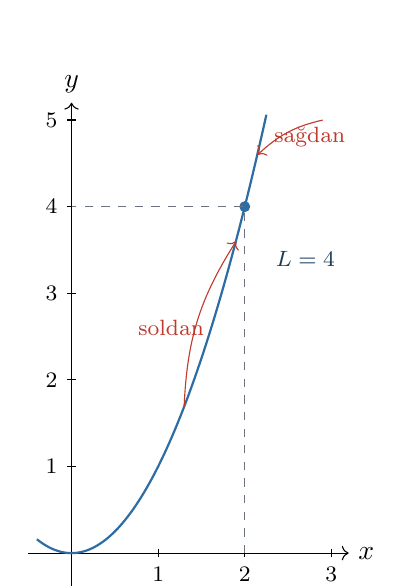
\begin{tikzpicture}[scale=1.1]
\draw[->] (-0.5,0)--(3.2,0) node[right]{$x$};
\draw[->] (0,-0.5)--(0,5.2) node[above]{$y$};
\foreach \x in {1,2,3} \draw (\x,0.05)--(\x,-0.05) node[below]{\footnotesize\x};
\foreach \y in {1,2,3,4,5} \draw (0.05,\y)--(-0.05,\y) node[left]{\footnotesize\y};
\draw[grafikMavi,thick,domain=-0.4:2.25,samples=100] plot (\x,{\x*\x});
\filldraw[grafikMavi] (2,4) circle (1.6pt);
\draw[dashed,ortaGri] (2,0)--(2,4)--(0,4);
\draw[->,kirmizi] (1.3,1.69) to[bend left=15] (1.9,3.6);
\draw[->,kirmizi] (2.9,5) to[bend right=15] (2.15,4.6);
\node[kirmizi] at (1.15,2.6) {\footnotesize soldan};
\node[kirmizi] at (2.75,4.8) {\footnotesize sağdan};
\node[anaMavi] at (2.7,3.4) {\footnotesize $L=4$};
\end{tikzpicture}
\end{center}

\gsub{Limiti Sayısal Olarak Görmek}

Limitin tanımındaki ``yaklaşma'' fikrini Python'la tablo hâlinde görebiliriz.
$f(x)=\dfrac{x^2-1}{x-1}$ fonksiyonu $x=1$'de tanımsızdır; ama limiti vardır.

\begin{lstlisting}
import numpy as np

def f(x):
    return (x**2 - 1)/(x - 1)

print(f"{'x':>10} {'f(x)':>12}")
for d in [0.1, 0.01, 0.001, 0.0001]:
    print(f"{1-d:>10.4f} {f(1-d):>12.6f}")     # soldan
for d in [0.0001, 0.001, 0.01, 0.1]:
    print(f"{1+d:>10.4f} {f(1+d):>12.6f}")     # sagdan
\end{lstlisting}

\begin{lstlisting}[style=outstyle]
         x         f(x)
    0.9000     1.900000
    0.9900     1.990000
    0.9990     1.999000
    0.9999     1.999900
    1.0001     2.000100
    1.0010     2.001000
    1.0100     2.010000
    1.1000     2.100000
\end{lstlisting}

İki taraftan da $2$'ye yaklaşıyor: $\lim_{x\to1}\frac{x^2-1}{x-1}=2$.

\begin{lstlisting}
import sympy as sp
x = sp.symbols('x')
sp.limit((x**2 - 1)/(x - 1), x, 1)      # 2
\end{lstlisting}

\uyari{Sayısal tablo bir \emph{kanıt} değildir. $f(x)=\sin(1/x)$ gibi
fonksiyonlarda tablo seni yanıltabilir; her zaman cebirsel/teorik doğrulama
yap.}

\gsub{Tek Taraflı Limitler (One-Sided Limits)}

\tanim{Soldan limit $\displaystyle\lim_{x\to a^-}f(x)$, yalnız $x<a$
değerleriyle; sağdan limit $\displaystyle\lim_{x\to a^+}f(x)$, yalnız $x>a$
değerleriyle hesaplanır.}

\kural[Temel Ölçüt]{Limitin var olması için iki taraflı limitlerin var
\emph{ve eşit} olması gerekir:
\[
\lm{x}{a} f(x)=L \iff \lim_{x\to a^-}f(x)=\lim_{x\to a^+}f(x)=L .
\]}

\begin{center}
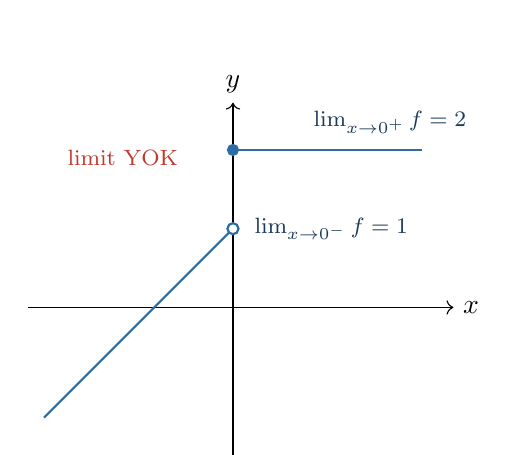
\begin{tikzpicture}[scale=1.0]
\draw[->] (-2.6,0)--(2.8,0) node[right]{$x$};
\draw[->] (0,-2.0)--(0,2.6) node[above]{$y$};
\draw[grafikMavi,thick] (-2.4,-1.4)--(0,1);
\draw[grafikMavi,thick] (0,2)--(2.4,2);
\filldraw[white,draw=grafikMavi,thick] (0,1) circle (2pt);
\filldraw[grafikMavi] (0,2) circle (2pt);
\node[anaMavi,right] at (0.15,1.0) {\footnotesize $\lim_{x\to0^-}f=1$};
\node[anaMavi,right] at (0.9,2.35) {\footnotesize $\lim_{x\to0^+}f=2$};
\node[kirmizi] at (-1.4,1.9) {\footnotesize limit YOK};
\end{tikzpicture}
\end{center}

\begin{lstlisting}
f = sp.Piecewise((x + 1, x < 0), (x + 2, True))

sp.limit(f, x, 0, '-')     # 1   (soldan)
sp.limit(f, x, 0, '+')     # 2   (sagdan)
sp.limit(f, x, 0)          # SymPy varsayilan olarak sagdan bakar!
\end{lstlisting}

\uyari{SymPy'de \code{sp.limit(f, x, a)} varsayılan olarak \emph{sağdan}
limittir (\code{dir='+'}). İki taraflı limit için \code{dir='+-'} kullan; limit
yoksa hata verir --- bu da limitin olmadığının işaretidir.}

\begin{lstlisting}
sp.limit(sp.Abs(x)/x, x, 0, '+')    #  1
sp.limit(sp.Abs(x)/x, x, 0, '-')    # -1
# sp.limit(sp.Abs(x)/x, x, 0, '+-') -> hata: limit yok
\end{lstlisting}

\gsub{Limit Kuralları (Limit Laws)}

$\lm{x}{a}f(x)=L$ ve $\lm{x}{a}g(x)=M$ olsun (ikisi de sonlu):

\begin{center}
\renewcommand{\arraystretch}{3.0}
\begin{tabularx}{\textwidth}{@{}>{\bfseries\color{anaMavi}}l >{$\displaystyle}X<{$}@{}}
\toprule
\rowcolor{acikMavi}\multicolumn{1}{@{}l}{\color{anaMavi}\textbf{Kural}} & \multicolumn{1}{l@{}}{\color{anaMavi}\textbf{Formül}}\\
\midrule
Toplam & \lm{x}{a}\bigl(f\pm g\bigr)=L\pm M\\
\rowcolor{acikGri} Sabit çarpan & \lm{x}{a} c\,f(x)=cL\\
Çarpım & \lm{x}{a}\bigl(f\cdot g\bigr)=L\cdot M\\
\rowcolor{acikGri} Bölüm & \lm{x}{a}\frac{f}{g}=\frac{L}{M},\quad M\neq 0\\
Kuvvet & \lm{x}{a}\bigl(f(x)\bigr)^n=L^n\\
\rowcolor{acikGri} Kök & \lm{x}{a}\sqrt[n]{f(x)}=\sqrt[n]{L}\\
Bileşke & \lm{x}{a} g(f(x))=g(L)\quad \text{($g$, $L$'de sürekli)}\\
\bottomrule
\end{tabularx}
\end{center}

\kural[Doğrudan Yerine Koyma]{$f$ polinom, rasyonel (paydası sıfır değilse),
kök, üstel, logaritmik veya trigonometrik gibi ``iyi huylu'' bir fonksiyonsa
ve $a$ tanım kümesindeyse:
\[ \lm{x}{a} f(x) = f(a). \]
Yani önce \emph{yerine koy}; sonuç bir sayıysa iş bitti.}

\gsub{Kesin Tanım: $\varepsilon$-$\delta$ (Epsilon-Delta)}

``Yaklaşıyor'' sözcüğü matematiksel değildir; Cauchy ve Weierstrass bu sezgiyi
kesin bir tanıma çevirmiştir.

\tanim[Kesin Limit Tanımı]{$\lm{x}{a}f(x)=L$ demek: \emph{her} $\varepsilon>0$
için \emph{öyle bir} $\delta>0$ vardır ki
\[
0<|x-a|<\delta \;\Longrightarrow\; |f(x)-L|<\varepsilon .
\]
Sezgisi: ``$f(x)$ değerini $L$'ye ne kadar ($\varepsilon$) yaklaştırmamı
istersen iste, ben sana $x$'in $a$'ya ne kadar ($\delta$) yaklaşması
gerektiğini söyleyebilirim.''}

\begin{center}
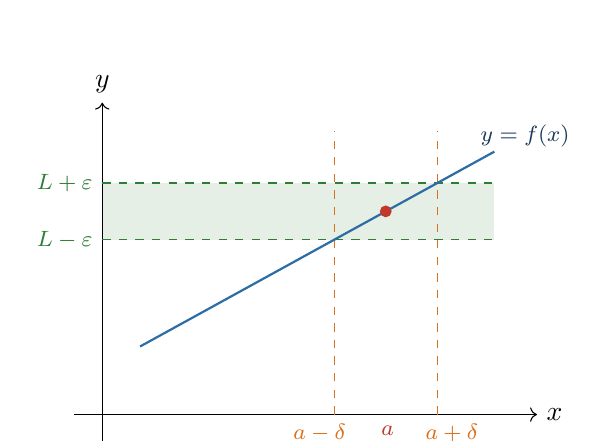
\begin{tikzpicture}[scale=1.2]
\fill[yesil!12] (0,1.85) rectangle (4.15,2.45);
\draw[->] (-0.3,0)--(4.6,0) node[right]{$x$};
\draw[->] (0,-0.3)--(0,3.3) node[above]{$y$};
\draw[dashed,yesil] (0,1.85)--(4.15,1.85);
\draw[dashed,yesil] (0,2.45)--(4.15,2.45);
\node[yesil,left] at (0,2.45) {\footnotesize $L+\varepsilon$};
\node[yesil,left] at (0,1.85) {\footnotesize $L-\varepsilon$};
\draw[dashed,turuncu] (2.455,0)--(2.455,3.0);
\draw[dashed,turuncu] (3.545,0)--(3.545,3.0);
\node[turuncu,below] at (2.3,0) {\footnotesize $a-\delta$};
\node[turuncu,below] at (3.7,0) {\footnotesize $a+\delta$};
\draw[grafikMavi,thick,domain=0.4:4.15,samples=60] plot (\x,{0.55*\x+0.5});
\filldraw[kirmizi] (3,2.15) circle (1.6pt);
\node[kirmizi,below] at (3.02,-0.02) {\footnotesize $a$};
\node[anaMavi,right] at (3.9,2.95) {\footnotesize $y=f(x)$};
\end{tikzpicture}
\end{center}

\soru{$\displaystyle\lm{x}{3}(2x-1)=5$ olduğunu $\varepsilon$-$\delta$
tanımıyla kanıtlayın.}

\cozum Verilen $\varepsilon>0$ için $|f(x)-5|<\varepsilon$ olmasını istiyoruz:
\[
|(2x-1)-5|=|2x-6|=2|x-3|<\varepsilon
\;\Longleftrightarrow\;
|x-3|<\frac{\varepsilon}{2}.
\]
O hâlde $\delta=\dfrac{\varepsilon}{2}$ seçmek yeterlidir: $0<|x-3|<\delta$
ise $|f(x)-5|=2|x-3|<2\delta=\varepsilon$. Kanıt tamamdır.

\ipucu{Doğrusal fonksiyonlarda $\delta=\varepsilon/|m|$ ($m$: eğim) her zaman
işe yarar. Doğrusal olmayanlarda önce $\delta\le1$ gibi bir ön kısıt koyup
ifadeyi sınırlamak standart hiledir.}

\begin{lstlisting}
import numpy as np

def delta_bul(f, a, L, eps, delta0=1.0, adim=0.99, ornek=20000):
    """Verilen eps icin gecerli bir delta'yi sayisal olarak arar."""
    d = delta0
    for _ in range(2000):
        xs = a + np.linspace(-d, d, ornek)
        xs = xs[np.abs(xs - a) > 1e-15]          # x = a haric
        if np.max(np.abs(f(xs) - L)) < eps:
            return d
        d *= adim
    return None

f = lambda x: 2*x - 1
for eps in [0.1, 0.01, 0.001]:
    d = delta_bul(f, 3, 5, eps)
    print(f"eps={eps:<7} delta={d:.6f}   (teorik: {eps/2})")
\end{lstlisting}

\begin{lstlisting}[style=outstyle]
eps=0.1     delta=0.049536   (teorik sinir: 0.05)
eps=0.01    delta=0.004959   (teorik sinir: 0.005)
eps=0.001   delta=0.000496   (teorik sinir: 0.0005)
\end{lstlisting}

\notk[Diğer Kesin Tanımlar]{Aynı mantık bütün limit türlerine uzanır:
\[
\lim_{x\to a}f(x)=\infty:\quad \forall M>0,\ \exists\delta>0:\
0<|x-a|<\delta \Rightarrow f(x)>M,
\]
\[
\lim_{x\to\infty}f(x)=L:\quad \forall\varepsilon>0,\ \exists N:\
x>N \Rightarrow |f(x)-L|<\varepsilon .
\]}

% =====================================================================
\gsec{Limit Hesaplama Teknikleri}
% =====================================================================

Yerine koyduğunda $\frac{0}{0}$ gibi bir \emph{belirsizlik} (indeterminate
form) çıkıyorsa, ifadeyi sadeleştirmen gerekir. Belirsizlik ``limit yok''
demek değildir; ``bu yolla bulunamaz, başka yol dene'' demektir.

\begin{center}
\begin{tabularx}{\textwidth}{@{}>{\bfseries\color{anaMavi}}l X@{}}
\toprule
\rowcolor{acikMavi}\multicolumn{1}{@{}l}{\color{anaMavi}\textbf{Biçim}} & \multicolumn{1}{l@{}}{\color{anaMavi}\textbf{Durum}}\\
\midrule
$0/0$, $\infty/\infty$ & Belirsiz --- sadeleştir veya L'Hôpital uygula.\\
\rowcolor{acikGri} $0\cdot\infty$, $\infty-\infty$ & Belirsiz --- kesir hâline getir.\\
$1^{\infty}$, $0^0$, $\infty^0$ & Belirsiz --- logaritma al.\\
\rowcolor{acikGri} $k/0$ ($k\neq0$) & Belirsiz \emph{değil}: $\pm\infty$ (işaret incelenir).\\
$\infty+\infty$, $\infty\cdot\infty$ & Belirsiz değil: $\infty$.\\
\bottomrule
\end{tabularx}
\end{center}

\gsub{Teknik 1: Çarpanlara Ayırma (Factoring)}

Pay ve paydada ortak çarpan varsa sadeleşir. $0/0$ veren rasyonel ifadelerde
ilk denenecek yöntemdir.

\soru{$\displaystyle \lm{x}{3}\frac{x^2-9}{x-3}$ limitini hesaplayın.}

\cozum Yerine koyarsak $\frac{0}{0}$: belirsiz. Payı çarpanlara ayıralım:
\[
\frac{x^2-9}{x-3}=\frac{(x-3)(x+3)}{x-3}=x+3 \quad (x\neq3).
\]
\[
\lm{x}{3}(x+3)=6.
\]

\pykontrol
\begin{lstlisting}
sp.factor(x**2 - 9)                  # (x - 3)*(x + 3)
sp.cancel((x**2 - 9)/(x - 3))        # x + 3
sp.limit((x**2 - 9)/(x - 3), x, 3)   # 6
\end{lstlisting}

\soru{$\displaystyle \lm{x}{2}\frac{x^3-8}{x^2-4}$ limitini hesaplayın.}

\cozum Küp farkı ve kare farkı özdeşlikleri:
\[
\frac{x^3-8}{x^2-4}=\frac{(x-2)(x^2+2x+4)}{(x-2)(x+2)}
=\frac{x^2+2x+4}{x+2}\ \longrightarrow\ \frac{4+4+4}{4}=3 .
\]

\gsub{Teknik 2: Eşlenikle Çarpma (Rationalizing)}

Kök içeren ifadelerde pay ve paydayı eşlenikle çarparız:
$(\sqrt{A}-\sqrt{B})(\sqrt{A}+\sqrt{B})=A-B$.

\soru{$\displaystyle \lm{x}{0}\frac{\sqrt{x+4}-2}{x}$ limitini hesaplayın.}

\cozum $\frac{0}{0}$ belirsizliği var. Eşlenik $\sqrt{x+4}+2$ ile çarpalım:
\[
\frac{\sqrt{x+4}-2}{x}\cdot\frac{\sqrt{x+4}+2}{\sqrt{x+4}+2}
=\frac{(x+4)-4}{x(\sqrt{x+4}+2)}=\frac{1}{\sqrt{x+4}+2}.
\]
$x\to0$ için sonuç $\dfrac{1}{2+2}=\dfrac{1}{4}$.

\pykontrol
\begin{lstlisting}
e = (sp.sqrt(x + 4) - 2)/x
sp.radsimp(e)                    # eslenikle rasyonellestirir
sp.limit(e, x, 0)                # 1/4
\end{lstlisting}

\gsub{Teknik 3: Ortak Payda ile Sadeleştirme}

$\infty-\infty$ veya iç içe kesir varsa önce tek kesir hâline getir.

\soru{$\displaystyle \lm{x}{0}\left(\frac{1}{x}-\frac{1}{x^2+x}\right)$
limitini hesaplayın.}

\cozum Ortak payda $x(x+1)$:
\[
\frac{1}{x}-\frac{1}{x(x+1)}=\frac{(x+1)-1}{x(x+1)}=\frac{x}{x(x+1)}
=\frac{1}{x+1}\ \longrightarrow\ 1 .
\]

\pykontrol
\begin{lstlisting}
e = 1/x - 1/(x**2 + x)
sp.together(e)        # x/(x*(x+1)) benzeri tek kesir
sp.limit(e, x, 0)     # 1
\end{lstlisting}

\gsub{Teknik 4: Mutlak Değer ve Parçalı Fonksiyonlar}

Mutlak değer içeren limitlerde \emph{mutlaka} tek taraflı bakılır.

\soru{$\displaystyle \lm{x}{2}\frac{|x-2|}{x-2}$ limitini inceleyin.}

\cozum $x>2$ iken $|x-2|=x-2$, oran $+1$; $x<2$ iken $|x-2|=-(x-2)$, oran
$-1$. Sağdan limit $1$, soldan limit $-1$; eşit olmadığı için \textbf{limit
yoktur}.

% =====================================================================
\gsec{Trigonometrik Limitler ve Sıkıştırma Teoremi}
% =====================================================================

\kural[Temel Trigonometrik Limitler]{
\[
\lm{x}{0}\frac{\sin x}{x}=1,\qquad
\lm{x}{0}\frac{\tan x}{x}=1,\qquad
\lm{x}{0}\frac{1-\cos x}{x}=0,\qquad
\lm{x}{0}\frac{1-\cos x}{x^2}=\frac12 .
\]
Bu limitler \emph{radyan} içindir; derece kullanılırsa sonuç değişir.}

Genelleştirme: $\lm{x}{0}\dfrac{\sin(kx)}{kx}=1$, yani
$\lm{x}{0}\dfrac{\sin(ax)}{bx}=\dfrac{a}{b}$.

\begin{center}
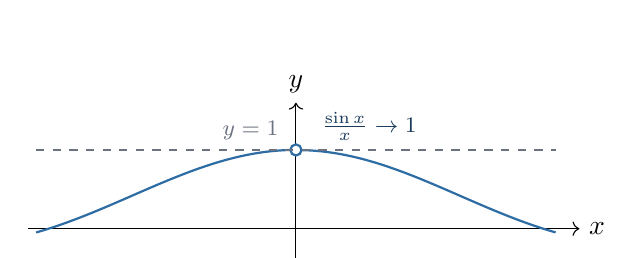
\begin{tikzpicture}[scale=1.0]
\draw[->] (-3.4,0)--(3.6,0) node[right]{$x$};
\draw[->] (0,-0.5)--(0,1.6) node[above]{$y$};
\draw[grafikMavi,thick,domain=-3.3:3.3,samples=200] plot (\x,{sin(deg(\x))/(\x+0.0001)});
\filldraw[white,draw=grafikMavi,thick] (0,1) circle (2pt);
\draw[dashed,ortaGri] (-3.3,1)--(3.3,1);
\node[anaMavi,right] at (0.2,1.3) {\footnotesize $\frac{\sin x}{x}\to 1$};
\node[ortaGri,left] at (-0.1,1.25) {\footnotesize $y=1$};
\end{tikzpicture}
\end{center}

\soru{$\displaystyle \lm{x}{0}\frac{\sin 5x}{3x}$ limitini hesaplayın.}

\cozum Pay ve paydayı düzenleyelim:
\[
\frac{\sin 5x}{3x}=\frac{5}{3}\cdot\frac{\sin 5x}{5x}
\ \longrightarrow\ \frac{5}{3}\cdot 1=\frac{5}{3}.
\]

\pykontrol
\begin{lstlisting}
sp.limit(sp.sin(5*x)/(3*x), x, 0)          # 5/3
sp.limit((1 - sp.cos(x))/x**2, x, 0)       # 1/2
sp.limit(sp.tan(x)/x, x, 0)                # 1
\end{lstlisting}

\gsub{Sıkıştırma Teoremi (Squeeze Theorem)}

\teorem{$a$ civarında $g(x)\le f(x)\le h(x)$ ve
$\lm{x}{a}g(x)=\lm{x}{a}h(x)=L$ ise, $\lm{x}{a}f(x)=L$ olmak zorundadır.}

\soru{$\displaystyle \lm{x}{0} x^2\sin\!\left(\frac{1}{x}\right)$ limitini
hesaplayın.}

\cozum $-1\le\sin(1/x)\le1$ olduğundan $x\neq0$ için
$-x^2\le x^2\sin(1/x)\le x^2$. Her iki uç da $x\to0$ iken $0$'a gider;
sıkıştırma teoremiyle limit $\boxed{0}$'dır.

\begin{lstlisting}
import numpy as np, matplotlib.pyplot as plt

xs = np.linspace(-0.5, 0.5, 4000)
xs = xs[xs != 0]
plt.plot(xs, xs**2*np.sin(1/xs), color='#2E6DA4', lw=1, label=r'$x^2\sin(1/x)$')
plt.plot(xs,  xs**2, 'r--', lw=1, label=r'$\pm x^2$')
plt.plot(xs, -xs**2, 'r--', lw=1)
plt.legend(); plt.grid(alpha=0.3); plt.show()

sp.limit(x**2*sp.sin(1/x), x, 0)      # 0
\end{lstlisting}

% =====================================================================
\gsec{Süreklilik (Continuity)}
% =====================================================================

\tanim{$f$ fonksiyonu $x=a$ noktasında \emph{süreklidir} eğer üç koşul birden
sağlanırsa:
\begin{enumerate}\itemsep1pt
\item $f(a)$ tanımlı,
\item $\lm{x}{a}f(x)$ var,
\item $\lm{x}{a}f(x)=f(a)$.
\end{enumerate}}

Sezgisel olarak: \emph{kalemi kaldırmadan çizebiliyorsan süreklidir.}

\gsub{Süreksizlik Türleri (Types of Discontinuity)}

\begin{center}
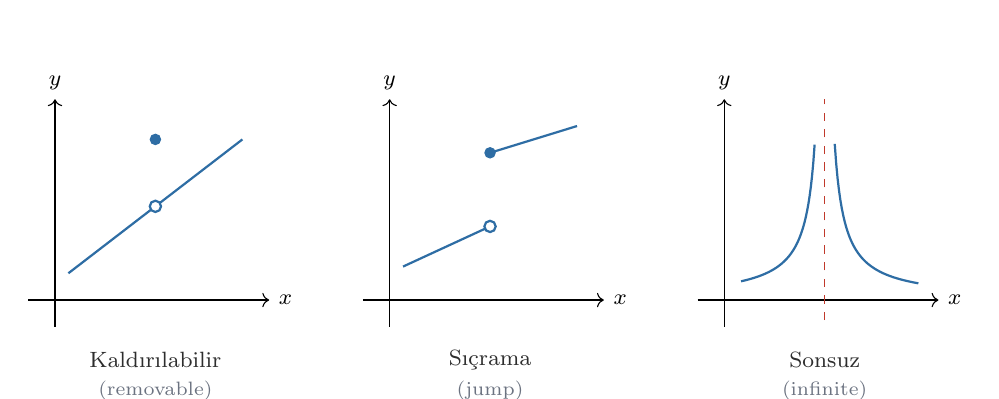
\begin{tikzpicture}[scale=0.85]
% Kaldirilabilir
\begin{scope}[xshift=0cm]
\draw[->] (-0.4,0)--(3.2,0) node[right]{\footnotesize $x$};
\draw[->] (0,-0.4)--(0,3.0) node[above]{\footnotesize $y$};
\draw[grafikMavi,thick] (0.2,0.4)--(2.8,2.4);
\filldraw[white,draw=grafikMavi,thick] (1.5,1.4) circle (2.4pt);
\filldraw[grafikMavi] (1.5,2.4) circle (2.2pt);
\node[koyuGri] at (1.5,-0.9) {\footnotesize Kaldırılabilir};
\node[ortaGri] at (1.5,-1.35) {\scriptsize (removable)};
\end{scope}
% Sicrama
\begin{scope}[xshift=5cm]
\draw[->] (-0.4,0)--(3.2,0) node[right]{\footnotesize $x$};
\draw[->] (0,-0.4)--(0,3.0) node[above]{\footnotesize $y$};
\draw[grafikMavi,thick] (0.2,0.5)--(1.5,1.1);
\draw[grafikMavi,thick] (1.5,2.2)--(2.8,2.6);
\filldraw[white,draw=grafikMavi,thick] (1.5,1.1) circle (2.4pt);
\filldraw[grafikMavi] (1.5,2.2) circle (2.2pt);
\node[koyuGri] at (1.5,-0.9) {\footnotesize Sıçrama};
\node[ortaGri] at (1.5,-1.35) {\scriptsize (jump)};
\end{scope}
% Sonsuz
\begin{scope}[xshift=10cm]
\draw[->] (-0.4,0)--(3.2,0) node[right]{\footnotesize $x$};
\draw[->] (0,-0.4)--(0,3.0) node[above]{\footnotesize $y$};
\draw[dashed,kirmizi] (1.5,-0.3)--(1.5,3.0);
\draw[grafikMavi,thick,domain=0.25:1.35,samples=60] plot (\x,{0.35/(1.5-\x)});
\draw[grafikMavi,thick,domain=1.65:2.9,samples=60] plot (\x,{0.35/(\x-1.5)});
\node[koyuGri] at (1.5,-0.9) {\footnotesize Sonsuz};
\node[ortaGri] at (1.5,-1.35) {\scriptsize (infinite)};
\end{scope}
\end{tikzpicture}
\end{center}
\vspace{1.1cm}

\begin{center}
\begin{tabularx}{\textwidth}{@{}>{\bfseries\color{anaMavi}}l X@{}}
\toprule
\rowcolor{acikMavi}\multicolumn{1}{@{}l}{\color{anaMavi}\textbf{Tür}} & \multicolumn{1}{l@{}}{\color{anaMavi}\textbf{Açıklama}}\\
\midrule
Kaldırılabilir & Limit var ama $f(a)$ ya yok ya farklı. Tek nokta yeniden tanımlanırsa süreklilik sağlanır.\\
\rowcolor{acikGri} Sıçrama & Sol ve sağ limitler var ama farklı. Parçalı fonksiyonlarda tipiktir.\\
Sonsuz & En az bir taraflı limit $\pm\infty$. Düşey asimptot vardır.\\
\rowcolor{acikGri} Salınımlı & $\sin(1/x)$ gibi; limit hiç oluşmaz.\\
\bottomrule
\end{tabularx}
\end{center}

\soru{$f(x)=\begin{cases} x^2+1, & x<2\\ k x, & x\ge 2\end{cases}$
fonksiyonunun $x=2$'de sürekli olması için $k$ kaç olmalıdır?}

\cozum Soldan limit: $2^2+1=5$. Sağdan limit ve değer: $2k$. Süreklilik için
$2k=5 \Rightarrow k=\dfrac{5}{2}$.

\pykontrol
\begin{lstlisting}
k = sp.symbols('k')
f = sp.Piecewise((x**2 + 1, x < 2), (k*x, True))

sol = sp.limit(f, x, 2, '-')          # 5
sag = sp.limit(f, x, 2, '+')          # 2*k
sp.solve(sp.Eq(sol, sag), k)          # [5/2]
\end{lstlisting}

\gsub{Ara Değer Teoremi (Intermediate Value Theorem)}

\teorem{$f$, $[a,b]$ üzerinde sürekli ve $N$ sayısı $f(a)$ ile $f(b)$ arasında
ise, $f(c)=N$ olacak en az bir $c\in(a,b)$ vardır. Özel hâli: $f(a)$ ve $f(b)$
zıt işaretliyse $(a,b)$ aralığında en az bir kök vardır.}

Bu teorem, kök bulmanın en temel sayısal yöntemi olan \emph{ikiye bölme}
(bisection) algoritmasının dayanağıdır.

\begin{lstlisting}
def bisection(f, a, b, tol=1e-10, maxit=200):
    """Ara Deger Teoremi'ne dayanan ikiye bolme yontemi."""
    fa, fb = f(a), f(b)
    if fa*fb > 0:
        raise ValueError("f(a) ve f(b) ayni isaretli: kok garanti degil")
    for _ in range(maxit):
        c = (a + b)/2
        fc = f(c)
        if abs(fc) < tol or (b - a)/2 < tol:
            return c
        if fa*fc < 0:
            b, fb = c, fc
        else:
            a, fa = c, fc
    return (a + b)/2

import numpy as np
kok = bisection(lambda t: t**3 - t - 2, 1, 2)
print(kok)                 # 1.5213797067990527
\end{lstlisting}

\begin{lstlisting}
# SciPy karsiligi
from scipy.optimize import brentq
brentq(lambda t: t**3 - t - 2, 1, 2)    # 1.5213797068045751
\end{lstlisting}

% =====================================================================
\gsec{Sonsuzda Limit ve Asimptotlar}
% =====================================================================

\gsub{Sonsuzda Limit (Limits at Infinity)}

$x\to\pm\infty$ iken fonksiyonun \emph{uç davranışını} (end behavior) sorarız.

\kural[Rasyonel Fonksiyonlarda Derece Kuralı]{$f(x)=\dfrac{P(x)}{Q(x)}$ olsun.
\[
\lim_{x\to\infty}\frac{P}{Q}=
\begin{cases}
0, & \deg P<\deg Q\\[4pt]
\dfrac{a_{\text{baş}}}{b_{\text{baş}}}, & \deg P=\deg Q\\[6pt]
\pm\infty, & \deg P>\deg Q
\end{cases}
\]
Pratik yöntem: paydadaki en büyük kuvvete böl.}

\soru{$\displaystyle \lim_{x\to\infty}\frac{3x^2-2x+1}{5x^2+7}$ nedir?}

\cozum Dereceler eşit; baş katsayıların oranı: $\dfrac{3}{5}$. Uzun yol:
$x^2$'ye bölersek $\dfrac{3-2/x+1/x^2}{5+7/x^2}\to\dfrac{3}{5}$.

\pykontrol
\begin{lstlisting}
sp.limit((3*x**2 - 2*x + 1)/(5*x**2 + 7), x,  sp.oo)   # 3/5
sp.limit((x**2 + 1)/(x**3 - 2),           x,  sp.oo)   # 0
sp.limit((x**3 + 1)/(x**2 + 1),           x,  sp.oo)   # oo
sp.limit(sp.exp(-x)*x**5,                 x,  sp.oo)   # 0
sp.limit((1 + 1/x)**x,                    x,  sp.oo)   # E
\end{lstlisting}

\uyari{Kök içeren sonsuz limitlerde $\sqrt{x^2}=|x|$ olduğunu unutma:
$x\to-\infty$ için $\sqrt{x^2}=-x$'tir. Bu yüzden
$\lim_{x\to-\infty}\frac{\sqrt{x^2+1}}{x}=-1$, ama
$\lim_{x\to+\infty}\frac{\sqrt{x^2+1}}{x}=+1$.}

\gsub{Bir Noktada Sonsuz Limit (Infinite Limits)}

\tanim{$\lim_{x\to a}f(x)=\infty$ yazmak ``limit sonsuz sayısına eşittir''
demek \emph{değildir}; limit yoktur ama fonksiyon \emph{sınırsız büyür}
demektir. Kesin olarak: her $M>0$ için, $0<|x-a|<\delta$ olduğunda $f(x)>M$
olacak bir $\delta>0$ vardır.}

Payda sıfıra giderken pay sıfırdan farklıysa sonuç $\pm\infty$'dur; işaret
için \emph{tek taraflı} bakmak zorunludur.

\begin{center}
\renewcommand{\arraystretch}{2.4}
\begin{tabularx}{\textwidth}{@{}>{$\displaystyle}X<{$} >{$\displaystyle}X<{$}@{}}
\toprule
\rowcolor{acikMavi}\multicolumn{1}{@{}l}{\color{anaMavi}\textbf{Limit}} & \multicolumn{1}{l@{}}{\color{anaMavi}\textbf{Karşılığı}}\\
\midrule
\lim_{x\to0^+}\frac{1}{x}=+\infty & \lim_{x\to0^-}\frac{1}{x}=-\infty\\
\rowcolor{acikGri} \lim_{x\to0}\frac{1}{x^2}=+\infty & \text{(iki taraf da aynı)}\\
\lim_{x\to0^+}\ln x=-\infty & \lim_{x\to(\pi/2)^-}\tan x=+\infty\\
\bottomrule
\end{tabularx}
\end{center}

\soru{$\displaystyle\lim_{x\to2^+}\frac{x+1}{x-2}$ ve
$\displaystyle\lim_{x\to2^-}\frac{x+1}{x-2}$ limitlerini bulun.}

\cozum Pay $x\to2$ iken $3>0$'a gider. Payda sağdan yaklaşırken küçük
\emph{pozitif}, soldan yaklaşırken küçük \emph{negatif} olur:
\[
\lim_{x\to2^+}\frac{x+1}{x-2}=+\infty,\qquad
\lim_{x\to2^-}\frac{x+1}{x-2}=-\infty .
\]
Demek ki $x=2$ bir düşey asimptottur.

\begin{lstlisting}
sp.limit((x + 1)/(x - 2), x, 2, '+')    #  oo
sp.limit((x + 1)/(x - 2), x, 2, '-')    # -oo
sp.limit(1/x**2, x, 0)                  #  oo
sp.limit(sp.log(x), x, 0, '+')          # -oo
sp.limit(sp.tan(x), x, sp.pi/2, '-')    #  oo
\end{lstlisting}

\gsub{Asimptotlar (Asymptotes)}

\begin{center}
\begin{tabularx}{\textwidth}{@{}>{\bfseries\color{anaMavi}}l X@{}}
\toprule
\rowcolor{acikMavi}\multicolumn{1}{@{}l}{\color{anaMavi}\textbf{Tür}} & \multicolumn{1}{l@{}}{\color{anaMavi}\textbf{Nasıl bulunur?}}\\
\midrule
Düşey ($x=a$) & $\lim_{x\to a^{\pm}}f(x)=\pm\infty$. Genelde paydanın kökleri (sadeleşmeyenler).\\
\rowcolor{acikGri} Yatay ($y=L$) & $\lim_{x\to\pm\infty}f(x)=L$ sonluysa.\\
Eğik ($y=mx+n$) & Pay derecesi paydadan 1 fazlaysa; bölme yaparak bul. $m=\lim\frac{f(x)}{x}$, $n=\lim (f(x)-mx)$.\\
\bottomrule
\end{tabularx}
\end{center}

\soru{$f(x)=\dfrac{x^2+1}{x-1}$ fonksiyonunun tüm asimptotlarını bulun.}

\cozum \textbf{Düşey:} $x=1$ (payda sıfır, pay $2\neq0$).
\textbf{Yatay:} yok (pay derecesi büyük).
\textbf{Eğik:} bölme yapalım:
$\dfrac{x^2+1}{x-1}=x+1+\dfrac{2}{x-1}$. Kalan terim $x\to\pm\infty$ iken
$0$'a gittiğinden eğik asimptot $y=x+1$'dir.

\pykontrol
\begin{lstlisting}
f = (x**2 + 1)/(x - 1)

sp.limit(f, x, 1, '+')      #  oo   -> dusey asimptot x = 1
sp.limit(f, x, 1, '-')      # -oo

m = sp.limit(f/x, x, sp.oo)         # 1
n = sp.limit(f - m*x, x, sp.oo)     # 1     -> egik asimptot y = x + 1
print(m, n)

sp.apart(f)                 # x + 1 + 2/(x - 1)  -> ayni sonuc
\end{lstlisting}

\ipucu{\code{sp.apart} bir rasyonel fonksiyonu ``polinom kısmı + kalan kesir''
biçiminde yazar. Polinom kısmı doğrudan eğik/yatay asimptotu verir. Bu, hem
asimptot bulmada hem de integral almada kullanılan aynı araçtır.}

% #####################################################################
\gpart{3}{Calculus 1 --- Türev (Derivative)}
% #####################################################################

% =====================================================================
\gsec{Türevin Tanımı ve Teğet Doğru}
% =====================================================================

Türev tek bir soruyu cevaplar: \textbf{``Bu fonksiyon şu anda ne kadar hızlı
değişiyor?''} Geometrik karşılığı teğetin eğimi, fiziksel karşılığı anlık
hızdır.

\gsub{Kesen Doğrudan Teğet Doğruya}

$(a,f(a))$ ve $(a+h,f(a+h))$ noktalarından geçen \emph{kesen} doğrunun eğimi
ortalama değişim oranıdır:
\[
m_{\text{kesen}}=\frac{f(a+h)-f(a)}{h}\qquad(\text{fark bölümü}).
\]
$h\to0$ yaparsak kesen doğru teğete dönüşür.

\begin{center}
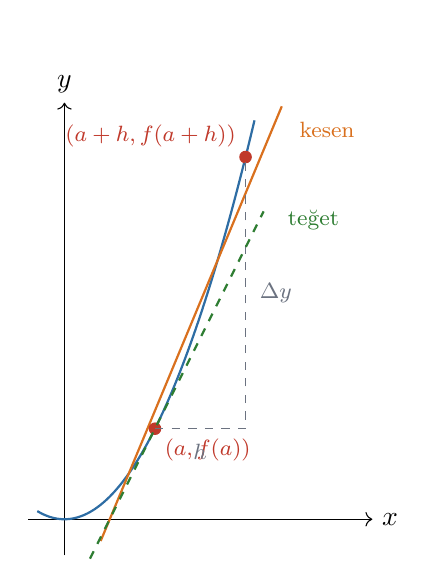
\begin{tikzpicture}[scale=1.15]
\draw[->] (-0.4,0)--(3.4,0) node[right]{$x$};
\draw[->] (0,-0.4)--(0,4.6) node[above]{$y$};
\draw[grafikMavi,thick,domain=-0.3:2.1,samples=100] plot (\x,{\x*\x});
% kesen
\draw[turuncu,thick] (0.4,-0.24)--(2.4,4.56);
\filldraw[kirmizi] (1,1) circle (1.8pt) node[below right]{\footnotesize $(a,f(a))$};
\filldraw[kirmizi] (2,4) circle (1.8pt) node[above left]{\footnotesize $(a+h,f(a+h))$};
\draw[dashed,ortaGri] (1,1)--(2,1)--(2,4);
\node[ortaGri] at (1.5,0.75) {\footnotesize $h$};
\node[ortaGri,right] at (2.05,2.5) {\footnotesize $\Delta y$};
% teget
\draw[yesil,thick,dashed] (0.2,-0.6)--(2.2,3.4);
\node[yesil] at (2.75,3.3) {\footnotesize teğet};
\node[turuncu] at (2.9,4.3) {\footnotesize kesen};
\end{tikzpicture}
\end{center}

\tanim[Türevin Tanımı]{
\[
f'(a)=\lim_{h\to0}\frac{f(a+h)-f(a)}{h}
     =\lim_{x\to a}\frac{f(x)-f(a)}{x-a},
\]
limit varsa $f$, $a$ noktasında \emph{türevlenebilirdir} (differentiable).}

\begin{center}
\begin{tabularx}{\textwidth}{@{}>{\bfseries\color{anaMavi}}l X@{}}
\toprule
\rowcolor{acikMavi}\multicolumn{1}{@{}l}{\color{anaMavi}\textbf{Gösterim}} & \multicolumn{1}{l@{}}{\color{anaMavi}\textbf{Okunuşu / kullanımı}}\\
\midrule
$f'(x)$ & Lagrange gösterimi; kısa ve yaygın.\\
\rowcolor{acikGri} $\dfrac{dy}{dx}$ & Leibniz; zincir kuralı ve değişken değiştirmede pratik.\\
$\dot{y}$ & Newton; fizikte zamana göre türev.\\
\rowcolor{acikGri} $D_x f$ & Operatör gösterimi.\\
\bottomrule
\end{tabularx}
\end{center}

\gsub{Tanımdan Türev Alma (First Principles)}

\soru{$f(x)=x^2$ için $f'(x)$'i tanımdan bulun.}

\cozum
\[
f'(x)=\lim_{h\to0}\frac{(x+h)^2-x^2}{h}
=\lim_{h\to0}\frac{2xh+h^2}{h}
=\lim_{h\to0}(2x+h)=2x .
\]

\pykontrol
\begin{lstlisting}
import sympy as sp
x, h = sp.symbols('x h')

f = lambda t: t**2
tanim = (f(x + h) - f(x))/h
sp.simplify(sp.limit(tanim, h, 0))       # 2*x

sp.diff(f(x), x)                          # 2*x   -> ayni sonuc
\end{lstlisting}

\begin{lstlisting}
def turev_tanimdan(ifade, degisken=x):
    """Tanimdan (limit ile) turev alan genel fonksiyon."""
    h = sp.symbols('h')
    return sp.simplify(sp.limit((ifade.subs(degisken, degisken + h) - ifade)/h, h, 0))

turev_tanimdan(sp.sqrt(x))        # 1/(2*sqrt(x))
turev_tanimdan(1/x)               # -1/x**2
turev_tanimdan(sp.sin(x))         # cos(x)
\end{lstlisting}

\gsub{Türevlenebilirlik ve Süreklilik}

\teorem{Türevlenebilen her fonksiyon süreklidir; tersi doğru değildir.
$f(x)=|x|$ fonksiyonu $x=0$'da süreklidir ama türevlenemez (sol türev $-1$,
sağ türev $+1$).}

Türevin olmadığı üç tipik durum: \textbf{köşe} ($|x|$), \textbf{düşey teğet}
($\sqrt[3]{x}$, $x=0$'da) ve \textbf{süreksizlik}.

\begin{center}
\begin{tikzpicture}[scale=0.9]
\begin{scope}
\draw[->] (-1.8,0)--(1.9,0) node[right]{\footnotesize $x$};
\draw[->] (0,-0.3)--(0,1.9) node[above]{\footnotesize $y$};
\draw[grafikMavi,thick] (-1.6,1.6)--(0,0)--(1.6,1.6);
\filldraw[kirmizi] (0,0) circle (2pt);
\node[koyuGri] at (0,-0.85) {\footnotesize köşe: $|x|$};
\end{scope}
\begin{scope}[xshift=5cm]
\draw[->] (-1.8,0)--(1.9,0) node[right]{\footnotesize $x$};
\draw[->] (0,-1.5)--(0,1.6) node[above]{\footnotesize $y$};
\draw[grafikMavi,thick,domain=0.001:1.6,samples=60] plot (\x,{pow(\x,0.3333)});
\draw[grafikMavi,thick,domain=0.001:1.6,samples=60] plot (-\x,{-pow(\x,0.3333)});
\filldraw[kirmizi] (0,0) circle (2pt);
\node[koyuGri] at (0,-2.1) {\footnotesize düşey teğet: $\sqrt[3]{x}$};
\end{scope}
\begin{scope}[xshift=10cm]
\draw[->] (-1.8,0)--(1.9,0) node[right]{\footnotesize $x$};
\draw[->] (0,-0.3)--(0,1.9) node[above]{\footnotesize $y$};
\draw[grafikMavi,thick] (-1.6,0.4)--(0,0.9);
\draw[grafikMavi,thick] (0,1.6)--(1.6,1.8);
\filldraw[white,draw=grafikMavi,thick] (0,0.9) circle (2pt);
\filldraw[grafikMavi] (0,1.6) circle (2pt);
\node[koyuGri] at (0,-0.85) {\footnotesize süreksizlik};
\end{scope}
\end{tikzpicture}
\end{center}
\vspace{0.7cm}

\gsub{Teğet Doğrunun Denklemi}

\kural{$(a,f(a))$ noktasındaki teğet doğrusu:
\[ y - f(a) = f'(a)\,(x-a). \]
Normal doğrusu (teğete dik) ise $y-f(a)=-\dfrac{1}{f'(a)}(x-a)$.}

\soru{$f(x)=x^3-2x$ eğrisinin $x=2$ noktasındaki teğet doğrusunu bulun.}

\cozum $f(2)=8-4=4$, $f'(x)=3x^2-2$, $f'(2)=10$. Teğet:
$y-4=10(x-2)\Rightarrow y=10x-16$.

\pykontrol
\begin{lstlisting}
import numpy as np, matplotlib.pyplot as plt

f = x**3 - 2*x
a = 2
m = sp.diff(f, x).subs(x, a)          # 10
y0 = f.subs(x, a)                      # 4
teget = y0 + m*(x - a)
sp.expand(teget)                       # 10*x - 16

fn = sp.lambdify(x, f, 'numpy')
tn = sp.lambdify(x, teget, 'numpy')
xs = np.linspace(0.5, 3, 200)
plt.plot(xs, fn(xs), lw=2, label='f(x)')
plt.plot(xs, tn(xs), '--', lw=2, label='teget')
plt.plot([a], [float(y0)], 'ro'); plt.legend(); plt.grid(alpha=0.3); plt.show()
\end{lstlisting}

\gsub{Sayısal Türev}

Sembolik türev her zaman mümkün olmayabilir (örneğin fonksiyon sadece ölçüm
verisi olarak varsa). O zaman fark formülleri kullanılır.

\begin{center}
\renewcommand{\arraystretch}{2.4}
\begin{tabularx}{\textwidth}{@{}>{\bfseries\color{anaMavi}}l >{$\displaystyle}l<{$} X@{}}
\toprule
\rowcolor{acikMavi}\multicolumn{1}{@{}l}{\color{anaMavi}\textbf{Formül}} & \multicolumn{1}{l}{\color{anaMavi}\textbf{İfade}} & \multicolumn{1}{l@{}}{\color{anaMavi}\textbf{Hata}}\\
\midrule
İleri fark & \frac{f(x+h)-f(x)}{h} & $O(h)$\\
\rowcolor{acikGri} Geri fark & \frac{f(x)-f(x-h)}{h} & $O(h)$\\
Merkezî fark & \frac{f(x+h)-f(x-h)}{2h} & $O(h^2)$ --- en iyisi\\
\rowcolor{acikGri} İkinci türev & \frac{f(x+h)-2f(x)+f(x-h)}{h^2} & $O(h^2)$\\
\bottomrule
\end{tabularx}
\end{center}

\begin{lstlisting}
import numpy as np

def turev_merkezi(f, x, h=1e-6):
    return (f(x + h) - f(x - h))/(2*h)

def ikinci_turev(f, x, h=1e-4):
    return (f(x + h) - 2*f(x) + f(x - h))/h**2

f = np.sin
print(turev_merkezi(f, 0.0))     # 0.9999999999998334  (cos 0 = 1)
print(ikinci_turev(f, 1.0))      # -0.8414709847...    (-sin 1)

# Veri uzerinde turev
xs = np.linspace(0, 2*np.pi, 100)
ys = np.sin(xs)
dydx = np.gradient(ys, xs)       # merkezi fark, uclarda tek yonlu
\end{lstlisting}

\uyari{$h$'yi çok küçültmek \emph{iyi değildir}: $10^{-12}$ gibi değerlerde
kayan nokta yuvarlama hatası baskın gelir ve sonuç bozulur. Merkezî fark için
$h\approx10^{-5}\ldots10^{-6}$ pratikte en iyi dengeyi verir.}

% =====================================================================
\gsec{Türev Kuralları}
% =====================================================================

\gsub{Temel Kurallar}

\begin{center}
\renewcommand{\arraystretch}{2.4}
\begin{tabularx}{\textwidth}{@{}>{\bfseries\color{anaMavi}}l >{$\displaystyle}X<{$}@{}}
\toprule
\rowcolor{acikMavi}\multicolumn{1}{@{}l}{\color{anaMavi}\textbf{Kural}} & \multicolumn{1}{l@{}}{\color{anaMavi}\textbf{Formül}}\\
\midrule
Sabit & \frac{d}{dx}(c)=0\\
\rowcolor{acikGri} Kuvvet (power) & \frac{d}{dx}(x^n)=n\,x^{n-1}\\
Sabit katı & \frac{d}{dx}\bigl(c\,f\bigr)=c\,f'\\
\rowcolor{acikGri} Toplam/fark & \bigl(f\pm g\bigr)'=f'\pm g'\\
Çarpım (product) & (f\cdot g)'=f'g+fg'\\
\rowcolor{acikGri} Bölüm (quotient) & \left(\frac{f}{g}\right)'=\frac{f'g-fg'}{g^2}\\
Zincir (chain) & \bigl(f(g(x))\bigr)'=f'(g(x))\cdot g'(x)\\
\bottomrule
\end{tabularx}
\end{center}

\ipucu{Bölüm kuralını ezberlemek için: ``\emph{pay türevi çarpı payda, eksi pay
çarpı payda türevi, bölü payda kare}''. Sıralamayı karıştırırsan işaret ters
çıkar --- bölüm kuralında sıra önemlidir, çarpım kuralında değildir.}

\soru{$f(x)=x^3\sin x$ fonksiyonunun türevini bulun.}

\cozum Çarpım kuralı: $f'=3x^2\sin x+x^3\cos x$.

\soru{$g(x)=\dfrac{x^2+1}{x-3}$ fonksiyonunun türevini bulun.}

\cozum Bölüm kuralı:
\[
g'=\frac{2x(x-3)-(x^2+1)\cdot1}{(x-3)^2}=\frac{x^2-6x-1}{(x-3)^2}.
\]

\pykontrol
\begin{lstlisting}
sp.diff(x**3*sp.sin(x), x)                    # x**3*cos(x) + 3*x**2*sin(x)
sp.simplify(sp.diff((x**2 + 1)/(x - 3), x))   # (x**2 - 6*x - 1)/(x - 3)**2
\end{lstlisting}

\gsub{Zincir Kuralı (Chain Rule)}

Bileşke fonksiyonların türevi. ``Dıştakinin türevi çarpı içtekinin türevi.''

\kural{$y=f(u)$ ve $u=g(x)$ ise
\[
\frac{dy}{dx}=\frac{dy}{du}\cdot\frac{du}{dx}
\qquad\text{yani}\qquad
\bigl(f(g(x))\bigr)'=f'(g(x))\cdot g'(x).
\]}

\soru{$y=\sin(3x^2+1)$ fonksiyonunun türevini bulun.}

\cozum Dış: $\sin u$, türevi $\cos u$. İç: $u=3x^2+1$, türevi $6x$.
\[ y'=\cos(3x^2+1)\cdot 6x = 6x\cos(3x^2+1). \]

\soru{$y=\left(x^2+1\right)^{10}$ türevini bulun.}

\cozum $y'=10(x^2+1)^9\cdot 2x=20x(x^2+1)^9$.

\pykontrol
\begin{lstlisting}
sp.diff(sp.sin(3*x**2 + 1), x)      # 6*x*cos(3*x**2 + 1)
sp.diff((x**2 + 1)**10, x)          # 20*x*(x**2 + 1)**9

# Ic ice zincir: 3 katmanli
sp.diff(sp.sin(sp.cos(sp.exp(x))), x)
# -exp(x)*sin(exp(x))*cos(cos(exp(x)))
\end{lstlisting}

% =====================================================================
\gsec{Trigonometrik, Üstel ve Logaritmik Türevler}
% =====================================================================

\gsub{Türev Tablosu}

\begin{center}
\renewcommand{\arraystretch}{2.4}
\begin{tabularx}{\textwidth}{@{}>{$\displaystyle}l<{$} >{$\displaystyle}l<{$} >{$\displaystyle}X<{$}@{}}
\toprule
\rowcolor{acikMavi}\multicolumn{1}{@{}l}{\color{anaMavi}\textbf{Fonksiyon}} & \multicolumn{1}{l}{\color{anaMavi}\textbf{Türevi}} & \multicolumn{1}{l@{}}{\color{anaMavi}\textbf{Zincirli hâli}}\\
\midrule
\sin x & \cos x & \bigl(\sin u\bigr)'=u'\cos u\\
\rowcolor{acikGri} \cos x & -\sin x & \bigl(\cos u\bigr)'=-u'\sin u\\
\tan x & \sec^2 x & \bigl(\tan u\bigr)'=u'\sec^2 u\\
\rowcolor{acikGri} \cot x & -\csc^2 x & \bigl(\cot u\bigr)'=-u'\csc^2 u\\
\sec x & \sec x\tan x & \bigl(\sec u\bigr)'=u'\sec u\tan u\\
\rowcolor{acikGri} \csc x & -\csc x\cot x & \bigl(\csc u\bigr)'=-u'\csc u\cot u\\
e^x & e^x & \bigl(e^u\bigr)'=u'e^u\\
\rowcolor{acikGri} a^x & a^x\ln a & \bigl(a^u\bigr)'=u'a^u\ln a\\
\ln x & \dfrac{1}{x} & \bigl(\ln u\bigr)'=\dfrac{u'}{u}\\
\rowcolor{acikGri} \log_a x & \dfrac{1}{x\ln a} & \bigl(\log_a u\bigr)'=\dfrac{u'}{u\ln a}\\
\arcsin x & \dfrac{1}{\sqrt{1-x^2}} & \bigl(\arcsin u\bigr)'=\dfrac{u'}{\sqrt{1-u^2}}\\
\rowcolor{acikGri} \arccos x & -\dfrac{1}{\sqrt{1-x^2}} & \bigl(\arccos u\bigr)'=-\dfrac{u'}{\sqrt{1-u^2}}\\
\arctan x & \dfrac{1}{1+x^2} & \bigl(\arctan u\bigr)'=\dfrac{u'}{1+u^2}\\
\rowcolor{acikGri} \sinh x & \cosh x & \bigl(\sinh u\bigr)'=u'\cosh u\\
\cosh x & \sinh x & \bigl(\cosh u\bigr)'=u'\sinh u\\
\rowcolor{acikGri} \tanh x & \operatorname{sech}^2 x & \bigl(\tanh u\bigr)'=u'\operatorname{sech}^2 u\\
\bottomrule
\end{tabularx}
\end{center}

\begin{lstlisting}
# Tabloyu Python ile uret ve dogrula
fonksiyonlar = [sp.sin(x), sp.cos(x), sp.tan(x), sp.exp(x), sp.log(x),
                sp.asin(x), sp.atan(x), sp.sinh(x), sp.tanh(x)]

for f in fonksiyonlar:
    print(f"{str(f):>12}  ->  {sp.simplify(sp.diff(f, x))}")
\end{lstlisting}

\begin{lstlisting}[style=outstyle]
      sin(x)  ->  cos(x)
      cos(x)  ->  -sin(x)
      tan(x)  ->  tan(x)**2 + 1
      exp(x)  ->  exp(x)
      log(x)  ->  1/x
     asin(x)  ->  1/sqrt(1 - x**2)
     atan(x)  ->  1/(x**2 + 1)
     sinh(x)  ->  cosh(x)
     tanh(x)  ->  1 - tanh(x)**2
\end{lstlisting}

\bilgi{SymPy $\sec^2x$ yerine $\tan^2x+1$ yazar; ikisi özdeştir. Beklediğin
biçimi elde etmek için \code{sp.simplify}, \code{sp.trigsimp} veya
\code{sp.rewrite} kullanabilirsin: \code{sp.diff(sp.tan(x),x).rewrite(sp.sec)}.}

\gsub{Kapalı Türev (Implicit Differentiation)}

$y$, $x$'in açık fonksiyonu olarak yazılamıyorsa (örneğin $x^2+y^2=25$), her
iki tarafın türevini alır, $y$'yi $x$'in fonksiyonu kabul ederiz; her $y$
türevinde zincir kuralı gereği $y'$ çarpanı çıkar.

\soru{$x^2+y^2=25$ çemberi için $\dfrac{dy}{dx}$'i bulun.}

\cozum
\[
2x+2y\,y'=0 \;\Longrightarrow\; y'=-\frac{x}{y}.
\]
Yani $(3,4)$ noktasında teğetin eğimi $-3/4$'tür.

\pykontrol
\begin{lstlisting}
x, y = sp.symbols('x y')

# 1. yol: idiff
sp.idiff(x**2 + y**2 - 25, y, x)          # -x/y

# 2. yol: y'yi fonksiyon yapip elle cozme
f = sp.Function('f')
denklem = sp.Eq(x**2 + f(x)**2, 25)
turevli = sp.diff(denklem, x)              # 2*x + 2*f(x)*Derivative(f(x), x) = 0
sp.solve(turevli, sp.Derivative(f(x), x))  # [-x/f(x)]
\end{lstlisting}

\soru{$x^3+y^3=6xy$ (Descartes yaprağı) eğrisinin $(3,3)$ noktasındaki teğet
eğimini bulun.}

\cozum Türev alalım: $3x^2+3y^2y'=6y+6xy'$. Düzenlersek
$y'(3y^2-6x)=6y-3x^2$, yani $y'=\dfrac{2y-x^2}{y^2-2x}$. $(3,3)$'te
$y'=\dfrac{6-9}{9-6}=-1$.

\begin{lstlisting}
m = sp.idiff(x**3 + y**3 - 6*x*y, y, x)
sp.simplify(m)                 # (-x**2 + 2*y)/(y**2 - 2*x)
m.subs({x: 3, y: 3})           # -1
\end{lstlisting}

\gsub{Logaritmik Türev}

Çok sayıda çarpan/bölüm içeren ya da $f(x)^{g(x)}$ biçimindeki ifadelerde önce
$\ln$ alınır.

\soru{$y=x^{x}$ fonksiyonunun türevini bulun.}

\cozum $\ln y=x\ln x$. Türev: $\dfrac{y'}{y}=\ln x+1$. Böylece
$y'=x^x(\ln x+1)$.

\pykontrol
\begin{lstlisting}
x = sp.symbols('x', positive=True)
sp.simplify(sp.diff(x**x, x))         # x**x*(log(x) + 1)
sp.diff(x**sp.sin(x), x)              # x**sin(x)*(sin(x)/x + log(x)*cos(x))
\end{lstlisting}

\gsub{Yüksek Mertebeden Türevler}

$f''=(f')'$, $f'''$, \dots, $f^{(n)}$. İkinci türev konkavlığı ve ivmeyi verir.

\begin{lstlisting}
x = sp.symbols('x')
f = x**5 - 3*x**3 + x

sp.diff(f, x, 2)          # 20*x**3 - 18*x
sp.diff(f, x, 3)          # 60*x**2 - 18

# n. turev formulu
n = sp.symbols('n', positive=True, integer=True)
[sp.diff(sp.exp(2*x), x, k) for k in range(4)]
# [exp(2*x), 2*exp(2*x), 4*exp(2*x), 8*exp(2*x)]  -> 2**n * exp(2x)
\end{lstlisting}

\ornek[Fizik Bağlantısı]{Konum $s(t)$ ise: hız $v=s'(t)$, ivme $a=s''(t)$,
sarsıntı (jerk) $j=s'''(t)$. Bir cismin \emph{yavaşlaması}, hız ile ivmenin
zıt işaretli olması demektir.}

% =====================================================================
\gsec{Ters ve Hiperbolik Fonksiyonların Türevi}
% =====================================================================

\gsub{Ters Fonksiyonun Türevi}

$f$ birebir ve türevlenebilirse, $f^{-1}$ de türevlenebilirdir. $y=f^{-1}(x)$
dersek $f(y)=x$ olur; her iki tarafın türevini alıp $y'$ çekeriz.

\kural{
\[
\bigl(f^{-1}\bigr)'(x)=\frac{1}{f'\bigl(f^{-1}(x)\bigr)}
\qquad\text{veya}\qquad
\frac{dy}{dx}=\frac{1}{dx/dy}.
\]
Geometrik anlamı: $f$ ile $f^{-1}$ grafikleri $y=x$'e göre simetriktir, bu
yüzden karşılıklı noktalardaki eğimler birbirinin tersidir.}

\soru{$f(x)=x^3+x+1$ olsun. $\bigl(f^{-1}\bigr)'(3)$ değerini bulun.}

\cozum Önce $f(a)=3$ olan $a$'yı bulalım: $a^3+a+1=3 \Rightarrow a=1$.
$f'(x)=3x^2+1$, $f'(1)=4$. O hâlde
\[
\bigl(f^{-1}\bigr)'(3)=\frac{1}{f'(1)}=\frac14 .
\]

\pykontrol
\begin{lstlisting}
import sympy as sp
x, y = sp.symbols('x y')

f = x**3 + x + 1
a = sp.solve(sp.Eq(f, 3), x)[0]        # 1
1/sp.diff(f, x).subs(x, a)             # 1/4
\end{lstlisting}

\ornek[Ters Trigonometrik Türevlerin Kaynağı]{$y=\arcsin x$ ise $\sin y=x$;
türev alırsak $\cos y\cdot y'=1$, yani $y'=\dfrac{1}{\cos y}
=\dfrac{1}{\sqrt{1-\sin^2y}}=\dfrac{1}{\sqrt{1-x^2}}$. Tablodaki bütün ters
trigonometrik türevler bu yolla elde edilir.}

\gsub{Hiperbolik Fonksiyonlar}

\tanim{
\[
\sinh x=\frac{e^x-e^{-x}}{2},\qquad
\cosh x=\frac{e^x+e^{-x}}{2},\qquad
\tanh x=\frac{\sinh x}{\cosh x}=\frac{e^{2x}-1}{e^{2x}+1}.
\]
Adları ``hiperbolik''tir çünkü $(\cosh t,\sinh t)$ noktası $x^2-y^2=1$
hiperbolünü çizer --- tıpkı $(\cos t,\sin t)$'nin çemberi çizmesi gibi.}

\begin{center}
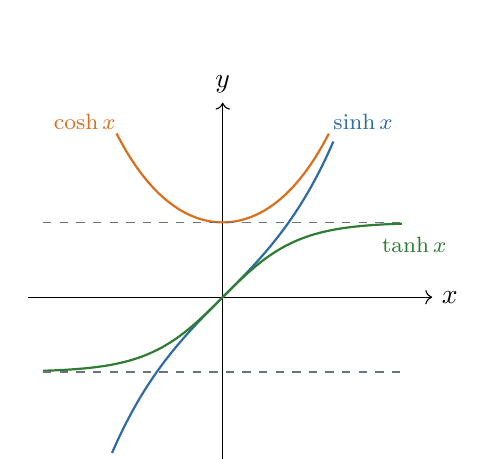
\begin{tikzpicture}[scale=0.95]
\draw[->] (-2.6,0)--(2.8,0) node[right]{$x$};
\draw[->] (0,-2.3)--(0,2.6) node[above]{$y$};
\draw[grafikMavi,thick,domain=-1.48:1.48,samples=80] plot (\x,{(exp(\x)-exp(-\x))/2});
\draw[turuncu,thick,domain=-1.42:1.42,samples=80] plot (\x,{(exp(\x)+exp(-\x))/2});
\draw[yesil,thick,domain=-2.4:2.4,samples=80] plot (\x,{(exp(2*\x)-1)/(exp(2*\x)+1)});
\draw[dashed,ortaGri] (-2.4,1)--(2.4,1);
\draw[dashed,ortaGri] (-2.4,-1)--(2.4,-1);
\node[grafikMavi,right] at (1.35,2.35) {\footnotesize $\sinh x$};
\node[turuncu,left] at (-1.3,2.35) {\footnotesize $\cosh x$};
\node[yesil,right] at (2.0,0.7) {\footnotesize $\tanh x$};
\end{tikzpicture}
\end{center}

\kural[Temel Özdeşlikler]{
\[
\cosh^2x-\sinh^2x=1,\qquad
1-\tanh^2x=\operatorname{sech}^2x,
\]
\[
\sinh(2x)=2\sinh x\cosh x,\qquad
\cosh(2x)=\cosh^2x+\sinh^2x .
\]
Trigonometrik özdeşliklerin işaret farkıyla aynısıdır (Osborn kuralı: iki
$\sinh$ çarpımı olan her terimin işareti değişir).}

\begin{center}
\renewcommand{\arraystretch}{2.4}
\begin{tabularx}{\textwidth}{@{}>{$\displaystyle}X<{$} >{$\displaystyle}X<{$}@{}}
\toprule
\rowcolor{acikMavi}\multicolumn{1}{@{}l}{\color{anaMavi}\textbf{Türev}} & \multicolumn{1}{l@{}}{\color{anaMavi}\textbf{Ters hiperbolik}}\\
\midrule
\bigl(\sinh x\bigr)'=\cosh x & \operatorname{arsinh}x=\ln\bigl(x+\sqrt{x^2+1}\bigr)\\
\rowcolor{acikGri} \bigl(\cosh x\bigr)'=\sinh x & \operatorname{arcosh}x=\ln\bigl(x+\sqrt{x^2-1}\bigr),\ x\ge1\\
\bigl(\tanh x\bigr)'=\operatorname{sech}^2x & \operatorname{artanh}x=\tfrac12\ln\dfrac{1+x}{1-x},\ |x|<1\\
\rowcolor{acikGri} \bigl(\operatorname{arsinh}x\bigr)'=\dfrac{1}{\sqrt{x^2+1}} & \bigl(\operatorname{artanh}x\bigr)'=\dfrac{1}{1-x^2}\\
\bottomrule
\end{tabularx}
\end{center}

\begin{lstlisting}
sp.diff(sp.sinh(x), x)                 # cosh(x)
sp.diff(sp.tanh(x), x)                 # 1 - tanh(x)**2
sp.simplify(sp.cosh(x)**2 - sp.sinh(x)**2)      # 1

sp.asinh(x).rewrite(sp.log)            # log(x + sqrt(x**2 + 1))
sp.diff(sp.asinh(x), x)                # 1/sqrt(x**2 + 1)

# Integral baglantisi: kok iceren integrallerin kapali cozumu
sp.integrate(1/sp.sqrt(x**2 + 1), x)   # asinh(x)
\end{lstlisting}

\ornek[Zincir Eğrisi (Catenary)]{İki uçtan asılan bir zincirin aldığı şekil
parabol değil, $y=a\cosh(x/a)$ eğrisidir. Bu yüzden $\cosh$ mühendislikte
(asma köprüler, elektrik hatları, St.\ Louis Gateway Arch) sürekli karşına
çıkar.}

% =====================================================================
\gsec{Doğrusal Hareket ve Marjinal Analiz}
% =====================================================================

\gsub{Doğrusal Hareket (Rectilinear Motion)}

\kural{Konum $s(t)$ ise: hız $v(t)=s'(t)$, sürat $|v(t)|$, ivme
$a(t)=v'(t)=s''(t)$.
\begin{itemize}\itemsep1pt
\item $v>0$: ileri, $v<0$: geri hareket.
\item $v$ ile $a$ \emph{aynı} işaretliyse cisim hızlanır, \emph{zıt}
işaretliyse yavaşlar.
\item Yer değiştirme $=\int v\dd t$, alınan yol $=\int|v|\dd t$.
\end{itemize}}

\soru{$s(t)=t^3-6t^2+9t$ (metre, $t\ge0$ saniye) hareketinde: (a) cisim ne
zaman ileri gider? (b) $[0,4]$ aralığında aldığı yol nedir?}

\cozum $v(t)=3t^2-12t+9=3(t-1)(t-3)$. $v>0$ iken $t<1$ veya $t>3$: cisim
$[0,1)$ ve $(3,4]$ aralıklarında ileri, $(1,3)$ aralığında geri gider.

Yol için $|v|$ integrali alınır; parçalara ayıralım:
$s(0)=0$, $s(1)=4$, $s(3)=0$, $s(4)=4$. Toplam yol
$|4-0|+|0-4|+|4-0|=12$ m. (Yer değiştirme ise yalnızca $4$ m'dir.)

\pykontrol
\begin{lstlisting}
t = sp.symbols('t', nonnegative=True)
s = t**3 - 6*t**2 + 9*t
v = sp.diff(s, t)                       # 3*t**2 - 12*t + 9
a = sp.diff(s, t, 2)                    # 6*t - 12

sp.solve(v, t)                          # [1, 3]  -> yon degisim anlari
sp.integrate(v, (t, 0, 4))              # 4       (yer degistirme)
sp.integrate(sp.Abs(v), (t, 0, 4))      # 12      (alinan yol)

# Hizlanma / yavaslama: v ve a ayni isaretli mi?
[(ti, v.subs(t, ti), a.subs(t, ti)) for ti in [0.5, 2, 3.5]]
\end{lstlisting}

\gsub{Ekonomide Marjinal Analiz}

\kural{$C(x)$ toplam maliyet ise \emph{marjinal maliyet} $C'(x)$'tir ve
``bir birim daha üretmenin yaklaşık maliyetidir'':
$C(x+1)-C(x)\approx C'(x)$. Benzer şekilde marjinal gelir $R'(x)$, marjinal
kâr $P'(x)=R'(x)-C'(x)$'tir. \textbf{Kâr, $R'(x)=C'(x)$ olduğunda
maksimumdur.}}

\soru{$C(x)=2000+3x+0{,}01x^2$ TL ve her ürün $23$ TL'ye satılıyorsa kârı
maksimize eden üretim miktarını bulun.}

\cozum $R(x)=23x$, $P(x)=R-C=-2000+20x-0{,}01x^2$.
$P'(x)=20-0{,}02x=0 \Rightarrow x=1000$ adet. $P''<0$ olduğundan maksimumdur;
$P(1000)=8000$ TL. Aynı sonuç $R'=C'$ koşulundan da gelir:
$23=3+0{,}02x$.

\begin{lstlisting}
x = sp.symbols('x', nonnegative=True)
C = 2000 + 3*x + sp.Rational(1,100)*x**2
R = 23*x
P = R - C

sp.solve(sp.diff(P, x), x)        # [1000]
P.subs(x, 1000)                    # 8000
sp.solve(sp.Eq(sp.diff(R, x), sp.diff(C, x)), x)   # [1000]  -> R' = C'
\end{lstlisting}

\notk[Ortalama Maliyet]{Ortalama maliyet $\bar{C}(x)=C(x)/x$ minimum olduğunda
$\bar{C}(x)=C'(x)$ olur --- yani ortalama maliyet eğrisi ile marjinal maliyet
eğrisi tam minimumda kesişir.}

% =====================================================================
\gsec{İlişkili Değişim Oranları (Related Rates)}
% =====================================================================

İki büyüklük bir denklemle bağlıysa, değişim hızları da bağlıdır. Yöntem:
\begin{enumerate}\itemsep1pt
\item Değişkenleri adlandır, şekil çiz.
\item Büyüklükler arasındaki \emph{denklemi} kur.
\item Denklemin \emph{zamana göre} türevini al (zincir kuralı!).
\item Bilinenleri yerine koy, aranan hızı çöz.
\end{enumerate}

\uyari{Sayısal değerleri türev almadan \emph{önce} yerine koyma. Önce genel
denklemin türevini al, \emph{sonra} anlık değerleri koy; aksi hâlde sabitleşen
değişkenlerin türevi sıfır çıkar.}

\soru{Yarıçapı $3$ cm/s hızla büyüyen bir dairenin alanı, yarıçap $10$ cm iken
ne hızla değişir?}

\cozum $A=\pi r^2$. Zamana göre türev: $\dfrac{dA}{dt}=2\pi r\dfrac{dr}{dt}$.
Yerine koyalım: $2\pi(10)(3)=60\pi\approx188.5$ cm$^2$/s.

\pykontrol
\begin{lstlisting}
t = sp.symbols('t')
r = sp.Function('r')(t)

A = sp.pi*r**2
dA = sp.diff(A, t)                        # 2*pi*r(t)*Derivative(r(t), t)

dA.subs({sp.Derivative(r, t): 3, r: 10})  # 60*pi
float(60*sp.pi)                            # 188.49555921538757
\end{lstlisting}

\soru{5 m uzunluğunda bir merdiven duvara dayalıdır. Alt ucu duvardan
$2$ m/s hızla uzaklaşırken, alt uç duvardan $3$ m uzaktayken üst uç ne hızla
aşağı iner?}

\cozum $x^2+y^2=25$. Türev: $2x x'+2y y'=0 \Rightarrow y'=-\dfrac{x x'}{y}$.
$x=3$ iken $y=4$; $y'=-\dfrac{3\cdot2}{4}=-1.5$ m/s (eksi işareti aşağı
yönü gösterir).

\begin{lstlisting}
xf = sp.Function('x')(t)
yf = sp.Function('y')(t)

eq = sp.Eq(xf**2 + yf**2, 25)
d  = sp.diff(eq, t)
dy = sp.solve(d, sp.Derivative(yf, t))[0]
dy.subs({xf: 3, yf: 4, sp.Derivative(xf, t): 2})    # -3/2
\end{lstlisting}

% =====================================================================
\gsec{Lineerleştirme, Diferansiyel ve Newton Yöntemi}
% =====================================================================

\gsub{Lineer Yaklaşım (Linearization)}

\kural{$a$ civarında $f(x)\approx L(x)=f(a)+f'(a)(x-a)$. Bu, teğet doğrusunun
fonksiyona yakın davranmasıdır --- Taylor serisinin birinci mertebeden hâli.}

\soru{$\sqrt{4.1}$ değerini lineer yaklaşımla tahmin edin.}

\cozum $f(x)=\sqrt{x}$, $a=4$: $f(4)=2$, $f'(x)=\frac{1}{2\sqrt x}$,
$f'(4)=\frac14$. Böylece $L(x)=2+\frac14(x-4)$ ve
$\sqrt{4.1}\approx2+0.025=2.025$. Gerçek değer $2.024845\ldots$

\pykontrol
\begin{lstlisting}
f = sp.sqrt(x); a = 4
L = f.subs(x, a) + sp.diff(f, x).subs(x, a)*(x - a)
L.subs(x, 4.1)              # 2.02500000000000
sp.sqrt(4.1).evalf()        # 2.02484567313166
\end{lstlisting}

\gsub{Diferansiyel}

$dy=f'(x)\,dx$: $x$'teki küçük bir $dx$ değişimine karşılık $y$'deki yaklaşık
değişim. Hata analizinde kullanılır.

\ornek{Yarıçapı $10\pm0.1$ cm ölçülen kürenin hacmindeki belirsizlik:
$V=\frac43\pi r^3$, $dV=4\pi r^2 dr=4\pi(100)(0.1)\approx125.7$ cm$^3$.
Bağıl hata: $\frac{dV}{V}=3\frac{dr}{r}=3\%$ --- yani yarıçaptaki $\%1$
hata hacimde $\%3$ hataya dönüşür.}

\gsub{Newton-Raphson Yöntemi}

Teğet doğrusunu kullanarak kök bulma:
\[
x_{n+1}=x_n-\frac{f(x_n)}{f'(x_n)} .
\]

\begin{center}
\begin{tikzpicture}[scale=1.0]
\draw[->] (-0.3,0)--(4.4,0) node[right]{$x$};
\draw[->] (0,-1.3)--(0,3.2) node[above]{$y$};
\draw[grafikMavi,thick,domain=0.3:4.0,samples=100] plot (\x,{0.35*(\x-1)*(\x-1)-0.9});
\filldraw[kirmizi] (3.6,{0.35*2.6*2.6-0.9}) circle (1.8pt) node[above right]{\footnotesize $x_n$};
\draw[turuncu,thick,dashed] (2.05,-1.25)--(4.1,2.6);
\filldraw[yesil] (2.72,0) circle (1.8pt) node[below]{\footnotesize $x_{n+1}$};
\filldraw[anaMavi] (2.6,0) circle (0pt);
\node[ortaGri] at (1.35,-1.1) {\footnotesize kök};
\end{tikzpicture}
\end{center}

\begin{lstlisting}
import sympy as sp

def newton(f_ifade, x0, degisken=None, tol=1e-12, maxit=50):
    """SymPy ifadesi icin Newton-Raphson kok bulma."""
    x = degisken or sp.symbols('x')
    f  = sp.lambdify(x, f_ifade, 'numpy')
    df = sp.lambdify(x, sp.diff(f_ifade, x), 'numpy')
    xn = float(x0)
    for i in range(maxit):
        fx = f(xn)
        if abs(fx) < tol:
            return xn, i
        xn = xn - fx/df(xn)
    return xn, maxit

x = sp.symbols('x')
kok, adim = newton(x**3 - x - 2, 1.5)
print(kok, adim)         # 1.5213797068045751  3
\end{lstlisting}

\uyari{Newton yöntemi hızlıdır (her adımda basamak sayısı yaklaşık ikiye
katlanır) ama $f'(x_n)\approx0$ olduğunda veya kötü bir başlangıç noktasında
ıraksayabilir. Güvenli alternatif: \code{scipy.optimize.brentq} (ikiye bölme
ile secant'ı birleştirir).}

% =====================================================================
\gsec{Ortalama Değer Teoremi ve Türevin Anlamı}
% =====================================================================

\teorem[Rolle Teoremi]{$f$, $[a,b]$'de sürekli, $(a,b)$'de türevlenebilir ve
$f(a)=f(b)$ ise, $f'(c)=0$ olacak en az bir $c\in(a,b)$ vardır.}

\teorem[Ortalama Değer Teoremi (MVT)]{$f$, $[a,b]$'de sürekli ve $(a,b)$'de
türevlenebilirse
\[
f'(c)=\frac{f(b)-f(a)}{b-a}
\]
olacak en az bir $c\in(a,b)$ vardır. Yani bir yerde anlık hız, ortalama hıza
eşit olmak zorundadır.}

\begin{center}
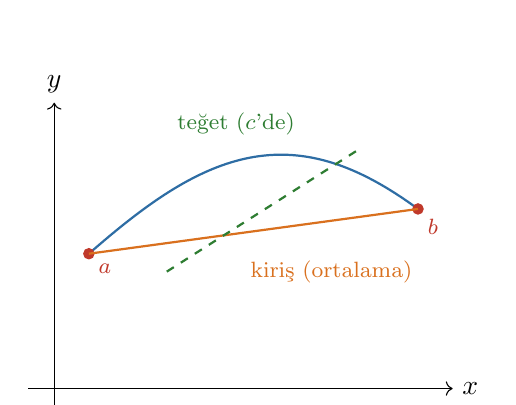
\begin{tikzpicture}[scale=1.1]
\draw[->] (-0.3,0)--(4.6,0) node[right]{$x$};
\draw[->] (0,-0.3)--(0,3.3) node[above]{$y$};
\draw[grafikMavi,thick,domain=0.4:4.2,samples=100] plot (\x,{1.2+1.5*sin(deg(0.6*\x))});
\filldraw[kirmizi] (0.4,{1.2+1.5*sin(deg(0.24))} ) circle (1.7pt) node[below right]{\footnotesize $a$};
\filldraw[kirmizi] (4.2,{1.2+1.5*sin(deg(2.52))} ) circle (1.7pt) node[below right]{\footnotesize $b$};
\draw[turuncu,thick] (0.4,{1.2+1.5*sin(deg(0.24))})--(4.2,{1.2+1.5*sin(deg(2.52))});
\draw[yesil,thick,dashed] (1.3,1.35)--(3.5,2.75);
\node[turuncu] at (3.2,1.35) {\footnotesize kiriş (ortalama)};
\node[yesil] at (2.1,3.05) {\footnotesize teğet ($c$'de)};
\end{tikzpicture}
\end{center}

\soru{$f(x)=x^2$ için $[1,3]$ aralığında MVT'yi sağlayan $c$ değerini bulun.}

\cozum $\dfrac{f(3)-f(1)}{3-1}=\dfrac{9-1}{2}=4$. $f'(c)=2c=4\Rightarrow c=2$.

\begin{lstlisting}
c = sp.symbols('c')
f = x**2; a, b = 1, 3
ort = (f.subs(x,b) - f.subs(x,a))/(b - a)          # 4
sp.solve(sp.Eq(sp.diff(f,x).subs(x,c), ort), c)    # [2]
\end{lstlisting}

\bilgi{MVT'nin en önemli sonucu: $f'(x)=0$ ise $f$ sabittir; $f'=g'$ ise
$f$ ile $g$ sabit farkla aynıdır. Bu, integralde ortaya çıkan ``$+C$''nin
teorik gerekçesidir.}

% =====================================================================
\gsec{Türev Uygulamaları: Ekstremum, Konkavlık, Eğri Çizimi}
% =====================================================================

\gsub{Artan/Azalan ve Kritik Noktalar}

\kural{$f'(x)>0$ ise $f$ artandır; $f'(x)<0$ ise azalandır. $f'(x)=0$ veya
$f'(x)$ tanımsız olan noktalara \emph{kritik nokta} denir; yerel ekstremumlar
yalnız kritik noktalarda olabilir.}

\kural[Birinci Türev Testi]{Kritik nokta $c$ civarında $f'$ işareti
$+\to-$ değişiyorsa yerel \textbf{maksimum}; $-\to+$ değişiyorsa yerel
\textbf{minimum}; işaret değişmiyorsa ekstremum yoktur.}

\kural[İkinci Türev Testi]{$f'(c)=0$ ve $f''(c)<0$ ise yerel maksimum;
$f''(c)>0$ ise yerel minimum. $f''(c)=0$ ise test sonuçsuzdur (birinci türev
testine dön).}

\soru{$f(x)=x^3-3x^2+1$ fonksiyonunun yerel ekstremumlarını bulun.}

\cozum $f'(x)=3x^2-6x=3x(x-2)$. Kritik noktalar: $x=0,\ x=2$.
$f''(x)=6x-6$; $f''(0)=-6<0$ (yerel maks, $f(0)=1$),
$f''(2)=6>0$ (yerel min, $f(2)=-3$).

\pykontrol
\begin{lstlisting}
f  = x**3 - 3*x**2 + 1
f1 = sp.diff(f, x)
f2 = sp.diff(f, x, 2)

kritik = sp.solve(f1, x)                # [0, 2]
for c in kritik:
    ikinci = f2.subs(x, c)
    tur = "yerel maks" if ikinci < 0 else ("yerel min" if ikinci > 0 else "belirsiz")
    print(f"x = {c}: f = {f.subs(x, c)}, f'' = {ikinci}  -> {tur}")
\end{lstlisting}

\begin{lstlisting}[style=outstyle]
x = 0: f = 1, f'' = -6  -> yerel maks
x = 2: f = -3, f'' = 6  -> yerel min
\end{lstlisting}

\gsub{Konkavlık ve Büküm Noktası (Concavity \& Inflection)}

\kural{$f''(x)>0$ ise grafik yukarı konkav (kâse gibi, $\smile$);
$f''(x)<0$ ise aşağı konkav ($\frown$). $f''$ işaret değiştirirse orası
\emph{büküm noktasıdır}.}

\begin{center}
\begin{tikzpicture}[scale=1.0]
\draw[->] (-2.6,0)--(2.8,0) node[right]{$x$};
\draw[->] (0,-2.2)--(0,2.4) node[above]{$y$};
\draw[grafikMavi,thick,domain=-1.9:1.9,samples=100] plot (\x,{0.32*\x*\x*\x});
\filldraw[kirmizi] (0,0) circle (2pt);
\node[kirmizi,above left] at (0,0.15) {\footnotesize büküm};
\node[ortaGri] at (-1.5,-1.8) {\footnotesize $f''<0$ ($\frown$)};
\node[ortaGri] at (1.5,1.9) {\footnotesize $f''>0$ ($\smile$)};
\end{tikzpicture}
\end{center}

\begin{lstlisting}
f = x**4 - 4*x**3
sp.solve(sp.diff(f, x, 2), x)      # [0, 2]  -> aday bukum noktalari

# Isaret degisimi kontrolu (bukum icin sart)
f2 = sp.diff(f, x, 2)
for c in [0, 2]:
    print(c, f2.subs(x, c - sp.Rational(1,10)), f2.subs(x, c + sp.Rational(1,10)))
\end{lstlisting}

\gsub{Mutlak Ekstremum (Kapalı Aralıkta)}

\kural[Kapalı Aralık Yöntemi]{$f$, $[a,b]$'de sürekliyse mutlak maksimum ve
minimum \emph{mutlaka} vardır. Adaylar: kritik noktalar ve uç noktalar
$a$, $b$. Hepsinin $f$ değerini hesapla, en büyüğü/küçüğü seç.}

\soru{$f(x)=x^3-3x$ fonksiyonunun $[-2,3]$ aralığındaki mutlak ekstremumlarını
bulun.}

\cozum $f'=3x^2-3=0\Rightarrow x=\pm1$. Adaylar $-2,-1,1,3$:
$f(-2)=-2$, $f(-1)=2$, $f(1)=-2$, $f(3)=18$. Mutlak maks $18$ ($x=3$),
mutlak min $-2$ ($x=-2$ ve $x=1$).

\begin{lstlisting}
f = x**3 - 3*x
a, b = -2, 3
adaylar = [a, b] + [c for c in sp.solve(sp.diff(f, x), x) if a <= c <= b]
degerler = {c: f.subs(x, c) for c in adaylar}
print(degerler)                      # {-2: -2, 3: 18, -1: 2, 1: -2}
print(max(degerler, key=degerler.get), min(degerler, key=degerler.get))
\end{lstlisting}

\gsub{Eğri Çizimi: Tam Analiz}

Bir fonksiyonun grafiğini elle çizmenin sistematik yolu:

\begin{center}
\begin{tabularx}{\textwidth}{@{}>{\bfseries\color{anaMavi}}c X@{}}
\toprule
\rowcolor{acikMavi}\multicolumn{1}{@{}c}{\color{anaMavi}\textbf{Adım}} & \multicolumn{1}{l@{}}{\color{anaMavi}\textbf{Ne yapılır?}}\\
\midrule
1 & Tanım kümesi, süreksizlikler.\\
\rowcolor{acikGri} 2 & Kesişimler: $f(0)$ ve $f(x)=0$ kökleri.\\
3 & Simetri: çift ($f(-x)=f(x)$), tek ($f(-x)=-f(x)$), periyodik.\\
\rowcolor{acikGri} 4 & Asimptotlar: düşey, yatay, eğik.\\
5 & $f'$: artan/azalan aralıklar, yerel ekstremumlar.\\
\rowcolor{acikGri} 6 & $f''$: konkavlık, büküm noktaları.\\
7 & Tabloyu birleştirip çiz.\\
\bottomrule
\end{tabularx}
\end{center}

\begin{lstlisting}
import numpy as np, matplotlib.pyplot as plt, sympy as sp
x = sp.symbols('x')

def egri_analizi(f, aralik=(-5, 5)):
    """Bir fonksiyonun tam turev analizini yapar ve grafigini cizer."""
    f1, f2 = sp.diff(f, x), sp.diff(f, x, 2)
    print("f      =", f)
    print("f'     =", sp.simplify(f1))
    print("f''    =", sp.simplify(f2))
    print("kokler =", sp.solve(f, x))
    print("kritik =", sp.solve(f1, x))
    print("bukum  =", sp.solve(f2, x))
    print("lim -oo=", sp.limit(f, x, -sp.oo), " lim +oo=", sp.limit(f, x, sp.oo))

    fn = sp.lambdify(x, f, 'numpy')
    xs = np.linspace(*aralik, 800)
    plt.plot(xs, fn(xs), lw=2, color='#2E6DA4')
    for c in sp.solve(f1, x):
        if c.is_real:
            plt.plot(float(c), float(f.subs(x, c)), 'ro')
    plt.axhline(0, color='gray', lw=0.8); plt.grid(alpha=0.3); plt.show()

egri_analizi(x**3 - 3*x**2 + 1, (-2, 4))
\end{lstlisting}

% =====================================================================
\gsec{Optimizasyon Problemleri}
% =====================================================================

Gerçek hayattaki ``en büyük/en küçük'' sorularının çözümü. Yöntem:
\begin{enumerate}\itemsep1pt
\item Optimize edilecek büyüklüğü bir denklemle yaz (\emph{amaç fonksiyonu}).
\item Kısıtı kullanarak tek değişkene indir.
\item Türevi sıfır yap, kritik noktaları bul.
\item Fiziksel tanım aralığını ve uç noktaları kontrol et.
\end{enumerate}

\soru{Çevresi $100$ m olan dikdörtgen bir bahçenin alanı en fazla kaç
m$^2$ olabilir?}

\cozum $2x+2y=100\Rightarrow y=50-x$. Alan: $A(x)=x(50-x)=50x-x^2$.
$A'=50-2x=0\Rightarrow x=25$. $A''=-2<0$: maksimum. $A(25)=625$ m$^2$
(kare!).

\pykontrol
\begin{lstlisting}
A = x*(50 - x)
kritik = sp.solve(sp.diff(A, x), x)      # [25]
A.subs(x, 25)                             # 625
sp.diff(A, x, 2)                          # -2  -> maksimum
\end{lstlisting}

\soru{Hacmi $1000$ cm$^3$ olan, üstü açık silindirik bir kabın malzemesi en az
olacak şekilde yarıçapını bulun.}

\cozum $V=\pi r^2h=1000\Rightarrow h=\dfrac{1000}{\pi r^2}$. Yüzey (taban +
yan): $S=\pi r^2+2\pi r h=\pi r^2+\dfrac{2000}{r}$.
$S'=2\pi r-\dfrac{2000}{r^2}=0\Rightarrow r^3=\dfrac{1000}{\pi}$,
$r=\sqrt[3]{1000/\pi}\approx6.83$ cm.

\begin{lstlisting}
r = sp.symbols('r', positive=True)
S = sp.pi*r**2 + 2000/r
kritik = sp.solve(sp.diff(S, r), r)      # [10/pi**(1/3)]
float(kritik[0])                          # 6.827840632552957
float(S.subs(r, kritik[0]))               # 439.4507...
\end{lstlisting}

\begin{lstlisting}
# Sayisal optimizasyon (SciPy) ile ayni sonuc
from scipy.optimize import minimize_scalar
import numpy as np

S_num = lambda r: np.pi*r**2 + 2000/r
sonuc = minimize_scalar(S_num, bounds=(0.1, 50), method='bounded')
print(sonuc.x, sonuc.fun)     # 6.8278406... 439.45072...
\end{lstlisting}

% =====================================================================
\gsec{L'Hôpital Kuralı}
% =====================================================================

\teorem[L'Hôpital]{$\lm{x}{a}\dfrac{f(x)}{g(x)}$ limiti $\dfrac{0}{0}$ veya
$\dfrac{\infty}{\infty}$ belirsizliği veriyorsa ve $g'(x)\neq0$ ise
\[
\lm{x}{a}\frac{f(x)}{g(x)}=\lm{x}{a}\frac{f'(x)}{g'(x)} .
\]
Sonuç yine belirsizse kural tekrar uygulanabilir.}

\uyari{L'Hôpital yalnız $0/0$ ve $\infty/\infty$ için geçerlidir. Belirsizlik
olmadan uygulamak \emph{yanlış} sonuç verir. Ayrıca bölümün türevi ile
karıştırma: pay ve payda \emph{ayrı ayrı} türevlenir.}

\soru{$\displaystyle \lm{x}{0}\frac{e^x-1-x}{x^2}$ limitini hesaplayın.}

\cozum $\frac00$: L'Hôpital $\Rightarrow \lm{x}{0}\dfrac{e^x-1}{2x}$; yine
$\frac00$: $\Rightarrow \lm{x}{0}\dfrac{e^x}{2}=\dfrac12$.

\pykontrol
\begin{lstlisting}
sp.limit((sp.exp(x) - 1 - x)/x**2, x, 0)      # 1/2

# Adim adim L'Hopital
pay, payda = sp.exp(x) - 1 - x, x**2
for i in range(3):
    print(f"adim {i}: {pay}/{payda}")
    if sp.limit(payda, x, 0) != 0:
        break
    pay, payda = sp.diff(pay, x), sp.diff(payda, x)
print("sonuc:", sp.limit(pay/payda, x, 0))
\end{lstlisting}

\gsub{Diğer Belirsizlikleri Dönüştürme}

\begin{center}
\begin{tabularx}{\textwidth}{@{}>{\bfseries\color{anaMavi}}c X@{}}
\toprule
\rowcolor{acikMavi}\multicolumn{1}{@{}c}{\color{anaMavi}\textbf{Biçim}} & \multicolumn{1}{l@{}}{\color{anaMavi}\textbf{Dönüşüm}}\\
\midrule
$0\cdot\infty$ & $f\cdot g=\dfrac{f}{1/g}$ yazarak $0/0$ yap.\\
\rowcolor{acikGri} $\infty-\infty$ & Ortak payda veya eşlenikle tek kesir yap.\\
$1^\infty,\ 0^0,\ \infty^0$ & $y=f^g$ için $\ln y=g\ln f$; limiti bul, sonra $e^{(\cdot)}$ al.\\
\bottomrule
\end{tabularx}
\end{center}

\soru{$\displaystyle \lim_{x\to\infty}\left(1+\frac{2}{x}\right)^{x}$ limitini
hesaplayın.}

\cozum $1^\infty$ belirsizliği. $\ln y=x\ln(1+2/x)$; $x\to\infty$ için bu
$\dfrac{\ln(1+2/x)}{1/x}\to\dfrac{0}{0}$, L'Hôpital ile $2$. O hâlde
$y\to e^2$.

\begin{lstlisting}
sp.limit((1 + 2/x)**x, x, sp.oo)          # exp(2)
sp.limit(x*sp.log(1 + 2/x), x, sp.oo)     # 2
sp.limit(x**x, x, 0, '+')                 # 1     (0^0 belirsizligi)
sp.limit(x**(1/x), x, sp.oo)              # 1     (oo^0 belirsizligi)
\end{lstlisting}

% #####################################################################
\gpart{4}{Calculus 1 --- İntegrale Giriş}
% #####################################################################

% =====================================================================
\gsec{Belirsiz İntegral (Antiderivative)}
% =====================================================================

İntegral, türevin ters işlemidir. ``Türevi $f(x)$ olan fonksiyon nedir?''
sorusunun cevabıdır.

\tanim{$F'(x)=f(x)$ ise $F$, $f$'nin bir \emph{ters türevidir}. Tüm ters
türevler sabit farkla birbirinden ayrılır:
\[
\int f(x)\dd x = F(x)+C .
\]}

\uyari{$+C$ unutulmaz. $\frac{d}{dx}(x^2)=2x$ ve $\frac{d}{dx}(x^2+7)=2x$
olduğundan $\int 2x\dd x = x^2+C$'dir. MVT'nin sonucu gereği, ters türevler
\emph{yalnızca} sabit kadar farklı olabilir.}

\gsub{Temel İntegral Kuralları}

\begin{center}
\renewcommand{\arraystretch}{3.0}
\begin{tabularx}{\textwidth}{@{}>{$\displaystyle}X<{$} >{$\displaystyle}X<{$}@{}}
\toprule
\rowcolor{acikMavi}\multicolumn{1}{@{}l}{\color{anaMavi}\textbf{İntegral}} & \multicolumn{1}{l@{}}{\color{anaMavi}\textbf{Sonuç}}\\
\midrule
\int x^n \dd x\ (n\neq-1) & \frac{x^{n+1}}{n+1}+C\\
\rowcolor{acikGri} \int \frac{1}{x}\dd x & \ln|x|+C\\
\int e^x \dd x & e^x+C\\
\rowcolor{acikGri} \int a^x \dd x & \frac{a^x}{\ln a}+C\\
\int \sin x \dd x & -\cos x+C\\
\rowcolor{acikGri} \int \cos x \dd x & \sin x+C\\
\int \sec^2 x \dd x & \tan x+C\\
\rowcolor{acikGri} \int \csc^2 x \dd x & -\cot x+C\\
\int \sec x\tan x \dd x & \sec x+C\\
\rowcolor{acikGri} \int \tan x \dd x & -\ln|\cos x|+C\\
\int \frac{1}{1+x^2}\dd x & \arctan x+C\\
\rowcolor{acikGri} \int \frac{1}{\sqrt{1-x^2}}\dd x & \arcsin x+C\\
\int \frac{1}{x\sqrt{x^2-1}}\dd x & \operatorname{arcsec}|x|+C\\
\bottomrule
\end{tabularx}
\end{center}

\ipucu{Her integral sonucunu \emph{türev alarak} kontrol edebilirsin. Bu,
kalkülüsün en güçlü öz-denetim mekanizmasıdır: \code{sp.diff(sp.integrate(f,
x), x)} her zaman \code{f}'e (sadeleştirildiğinde) eşit olmalıdır.}

\begin{lstlisting}
import sympy as sp
x = sp.symbols('x')

F = sp.integrate(x**3 + 2*x, x)       # x**4/4 + x**2
sp.simplify(sp.diff(F, x))            # x**3 + 2*x   -> dogrulandi

sp.integrate(1/x, x)                  # log(x)   (SymPy mutlak deger yazmaz)
sp.integrate(sp.exp(3*x), x)          # exp(3*x)/3
sp.integrate(sp.sin(x)*sp.cos(x), x)  # sin(x)**2/2
\end{lstlisting}

\uyari{SymPy $\int\frac1x dx$ için $\ln x$ yazar, $\ln|x|$ değil; çünkü
karmaşık düzlemde çalışır. Kâğıt üzerinde \emph{mutlak değeri} yazmayı unutma.
Ayrıca SymPy $+C$ eklemez.}

\gsub{Doğrusallık}

\[
\int \bigl(a f(x)+b g(x)\bigr)\dd x = a\int f(x)\dd x + b\int g(x)\dd x .
\]

\uyari{Çarpım ve bölümün integrali, integrallerin çarpımı/bölümü
\textbf{değildir}. $\int f g \neq \int f \cdot \int g$. Bu tür integraller
için kısmi integral veya yerine koyma gerekir (Kısım 5).}

\soru{$\displaystyle\int\left(3x^2-\frac{4}{x}+\sqrt{x}\right)dx$ integralini
hesaplayın.}

\cozum Terim terim:
\[
3\cdot\frac{x^3}{3}-4\ln|x|+\frac{x^{3/2}}{3/2}+C
= x^3-4\ln|x|+\frac{2}{3}x^{3/2}+C .
\]

\begin{lstlisting}
sp.integrate(3*x**2 - 4/x + sp.sqrt(x), x)
# x**3 + 2*x**(3/2)/3 - 4*log(x)
\end{lstlisting}

\gsub{Başlangıç Koşullu Problemler (İlkel Fonksiyon Bulma)}

Türevi verilen bir fonksiyonu bulurken $+C$ belirsiz kalır; bir \emph{başlangıç
koşulu} ($f(x_0)=y_0$) verilirse $C$ tek bir değere sabitlenir.

\soru{$f'(x)=3x^2-2$ ve $f(1)=4$ ise $f(x)$ nedir?}

\cozum $f(x)=x^3-2x+C$. $f(1)=1-2+C=4 \Rightarrow C=5$. Yani
$f(x)=x^3-2x+5$.

\soru{Bir top yerden $20$ m/s hızla yukarı atılıyor ($a=-9{,}8$ m/s$^2$).
Ulaştığı maksimum yüksekliği bulun.}

\cozum $v(t)=-9{,}8t+20$ (çünkü $v(0)=20$), $s(t)=-4{,}9t^2+20t$ (çünkü
$s(0)=0$). Maksimum yükseklik $v=0$ anındadır: $t=20/9{,}8\approx2{,}04$ s.
\[
s(2{,}04)=\frac{20^2}{2\cdot9{,}8}\approx20{,}41\ \text{m}.
\]

\pykontrol
\begin{lstlisting}
t, C1, C2 = sp.symbols('t C1 C2')

v = sp.integrate(-9.8, t) + C1                 # -9.8*t + C1
v = v.subs(C1, 20)                              # v(0) = 20
s = sp.integrate(v, t) + C2
s = s.subs(C2, 0)                               # s(0) = 0

t_tepe = sp.solve(v, t)[0]                      # 2.0408163265306
s.subs(t, t_tepe)                               # 20.4081632653061
\end{lstlisting}

\begin{lstlisting}
# Ayni is diferansiyel denklem cozucusuyle
x = sp.symbols('x')
f = sp.Function('f')
sp.dsolve(sp.Eq(f(x).diff(x), 3*x**2 - 2), f(x), ics={f(1): 4})
# Eq(f(x), x**3 - 2*x + 5)
\end{lstlisting}

% =====================================================================
\gsec{Riemann Toplamı ve Belirli İntegral}
% =====================================================================

Belirli integral, bir eğrinin altındaki \emph{alanı} (işaretli alan) verir.
Fikir: bölgeyi ince dikdörtgenlere böl, alanlarını topla, dikdörtgen sayısını
sonsuza götür.

\gsub{Riemann Toplamı}

$[a,b]$ aralığını $n$ eşit parçaya böl: $\Delta x=\dfrac{b-a}{n}$,
$x_i=a+i\Delta x$.

\[
\text{Sol: } \sum_{i=0}^{n-1}f(x_i)\Delta x,\qquad
\text{Sağ: } \sum_{i=1}^{n}f(x_i)\Delta x,\qquad
\text{Orta: } \sum_{i=1}^{n}f\!\left(\tfrac{x_{i-1}+x_i}{2}\right)\Delta x .
\]

\tanim[Belirli İntegral]{
\[
\int_a^b f(x)\dd x=\lim_{n\to\infty}\sum_{i=1}^{n}f(x_i^*)\,\Delta x .
\]}

\begin{center}
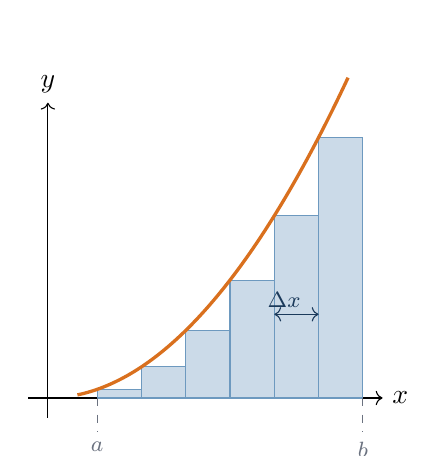
\begin{tikzpicture}[scale=1.25]
\draw[->] (-0.2,0)--(3.4,0) node[right]{$x$};
\draw[->] (0,-0.2)--(0,3.0) node[above]{$y$};
\foreach \i in {0,1,2,3,4,5}{
  \pgfmathsetmacro{\xa}{0.5+\i*0.45}
  \pgfmathsetmacro{\hh}{0.35*\xa*\xa}
  \filldraw[grafikMavi!25,draw=grafikMavi!70] (\xa,0) rectangle ({\xa+0.45},\hh);
}
\draw[turuncu,very thick,domain=0.3:3.05,samples=100] plot (\x,{0.35*\x*\x});
\draw[dashed,ortaGri] (0.5,0)--(0.5,-0.35) node[below]{\footnotesize $a$};
\draw[dashed,ortaGri] (3.2,0)--(3.2,-0.35) node[below]{\footnotesize $b$};
\node[anaMavi] at (2.4,1.0) {\footnotesize $\Delta x$};
\draw[<->,anaMavi] (2.3,0.85)--(2.75,0.85);
\end{tikzpicture}
\end{center}

\begin{lstlisting}
import numpy as np

def riemann(f, a, b, n, tur='orta'):
    """Sol, sag, orta ve yamuk Riemann toplamlari."""
    xs = np.linspace(a, b, n + 1)
    dx = (b - a)/n
    if tur == 'sol':
        return np.sum(f(xs[:-1]))*dx
    if tur == 'sag':
        return np.sum(f(xs[1:]))*dx
    if tur == 'orta':
        return np.sum(f((xs[:-1] + xs[1:])/2))*dx
    if tur == 'yamuk':
        return np.trapz(f(xs), xs)
    raise ValueError(tur)

f = lambda t: t**2
for n in [10, 100, 1000, 100000]:
    print(f"n={n:>6}  sol={riemann(f,0,1,n,'sol'):.8f}  "
          f"orta={riemann(f,0,1,n,'orta'):.8f}  sag={riemann(f,0,1,n,'sag'):.8f}")
\end{lstlisting}

\begin{lstlisting}[style=outstyle]
n=    10  sol=0.28500000  orta=0.33250000  sag=0.38500000
n=   100  sol=0.32835000  orta=0.33332500  sag=0.33835000
n=  1000  sol=0.33283350  orta=0.33333325  sag=0.33383350
n=100000  sol=0.33332833  orta=0.33333333  sag=0.33333833
\end{lstlisting}

Gerçek değer $\int_0^1 x^2 dx=\frac13$. Görüldüğü gibi orta nokta kuralı çok
daha hızlı yakınsar.

\gsub{Riemann Toplamını Sembolik Olarak Almak}

\begin{lstlisting}
i, n = sp.symbols('i n', positive=True, integer=True)
a, b = 0, 1
dx = (b - a)/n
xi = a + i*dx

toplam = sp.summation((xi**2)*dx, (i, 1, n))     # (n+1)*(2n+1)/(6n**2) benzeri
sp.simplify(toplam)
sp.limit(sp.simplify(toplam), n, sp.oo)          # 1/3   -> tanimdan integral
\end{lstlisting}

\gsub{Belirli İntegralin Özellikleri}

\begin{center}
\renewcommand{\arraystretch}{3.0}
\begin{tabularx}{\textwidth}{@{}>{\bfseries\color{anaMavi}}l >{$\displaystyle}X<{$}@{}}
\toprule
\rowcolor{acikMavi}\multicolumn{1}{@{}l}{\color{anaMavi}\textbf{Özellik}} & \multicolumn{1}{l@{}}{\color{anaMavi}\textbf{Formül}}\\
\midrule
Ters sınır & \int_a^b f=-\int_b^a f\\
\rowcolor{acikGri} Aynı sınır & \int_a^a f=0\\
Bölme & \int_a^b f=\int_a^c f+\int_c^b f\\
\rowcolor{acikGri} Doğrusallık & \int_a^b (cf+dg)=c\int_a^b f+d\int_a^b g\\
Karşılaştırma & f\le g \Rightarrow \int_a^b f\le\int_a^b g\\
\rowcolor{acikGri} Tek fonksiyon & \int_{-a}^{a} f=0\quad (f(-x)=-f(x))\\
Çift fonksiyon & \int_{-a}^{a} f=2\int_0^a f\quad (f(-x)=f(x))\\
\bottomrule
\end{tabularx}
\end{center}

\ipucu{Simetri özelliği sınavda büyük zaman kazandırır: $\int_{-2}^{2}
x^3\cos x\dd x$ integrali, integrand tek fonksiyon olduğu için doğrudan
$0$'dır --- hiç hesap yapmadan.}

\begin{lstlisting}
sp.integrate(x**3*sp.cos(x), (x, -2, 2))     # 0
sp.integrate(x**2, (x, -2, 2))               # 16/3  = 2 * integral(0..2)
\end{lstlisting}

% =====================================================================
\gsec{Kalkülüsün Temel Teoremi (Fundamental Theorem of Calculus)}
% =====================================================================

Türev ve integrali birbirine bağlayan, kalkülüsün en önemli teoremi.

\teorem[FTC --- 1. Kısım]{$f$, $[a,b]$'de sürekli ve
$\displaystyle g(x)=\int_a^x f(t)\dd t$ ise $g$ türevlenebilirdir ve
\[
g'(x)=f(x).
\]
Yani ``integralin türevi, fonksiyonun kendisidir''.}

\teorem[FTC --- 2. Kısım]{$F$, $f$'nin herhangi bir ters türeviyse
\[
\int_a^b f(x)\dd x=F(b)-F(a)=\Bigl[F(x)\Bigr]_a^b .
\]}

\kural[Zincirli FTC]{
\[
\frac{d}{dx}\int_{u(x)}^{v(x)} f(t)\dd t = f(v(x))\,v'(x)-f(u(x))\,u'(x).
\]}

\soru{$\displaystyle g(x)=\int_1^{x^2}\sqrt{1+t^3}\;dt$ ise $g'(x)$ nedir?}

\cozum Üst sınır $x^2$, zincir kuralıyla:
$g'(x)=\sqrt{1+(x^2)^3}\cdot 2x = 2x\sqrt{1+x^6}$.

\pykontrol
\begin{lstlisting}
t = sp.symbols('t')
g = sp.Integral(sp.sqrt(1 + t**3), (t, 1, x**2))

sp.diff(g, x)          # 2*x*sqrt(x**6 + 1)   -> zincirli FTC
# Not: g.doit() kapali formda cozulemez ama turevi kolayca alinir.
\end{lstlisting}

\soru{$\displaystyle\int_0^{2}(3x^2+1)\,dx$ integralini hesaplayın.}

\cozum $F(x)=x^3+x$. $F(2)-F(0)=(8+2)-0=10$.

\begin{lstlisting}
sp.integrate(3*x**2 + 1, (x, 0, 2))     # 10

# Sayisal karsilastirma
from scipy.integrate import quad
quad(lambda u: 3*u**2 + 1, 0, 2)        # (10.000000000000002, 1.1e-13)
\end{lstlisting}

\bilgi{\code{scipy.integrate.quad} bir demet döndürür: \code{(değer,
tahmini\_hata)}. Sembolik integral bulunamadığında (ki çoğu gerçek problemde
bulunamaz) doğru araç budur.}

% =====================================================================
\gsec{Yerine Koyma Yöntemi (u-Substitution)}
% =====================================================================

Zincir kuralının tersidir. $\int f(g(x))g'(x)\dd x$ biçimindeki integrallerde
$u=g(x)$, $du=g'(x)dx$ dönüşümü yapılır.

\kural{
\[
\int f(g(x))\,g'(x)\dd x = \int f(u)\dd u \quad\text{ve}\quad
\int_a^b f(g(x))g'(x)\dd x=\int_{g(a)}^{g(b)} f(u)\dd u .
\]
Belirli integralde \emph{sınırları da dönüştürürsen} geri dönmene gerek kalmaz.}

\soru{$\displaystyle\int 2x\,e^{x^2}dx$ integralini hesaplayın.}

\cozum $u=x^2$, $du=2x\,dx$:
$\int e^u du=e^u+C=e^{x^2}+C$.

\soru{$\displaystyle\int_0^{\pi/2}\sin^3 x\cos x\;dx$ integralini hesaplayın.}

\cozum $u=\sin x$, $du=\cos x\,dx$. Sınırlar: $x=0\Rightarrow u=0$;
$x=\pi/2\Rightarrow u=1$.
\[
\int_0^1 u^3du=\left[\frac{u^4}{4}\right]_0^1=\frac14 .
\]

\pykontrol
\begin{lstlisting}
sp.integrate(2*x*sp.exp(x**2), x)                        # exp(x**2)
sp.integrate(sp.sin(x)**3*sp.cos(x), (x, 0, sp.pi/2))    # 1/4

# SymPy'ye degisken degistirtmek (adim adim gormek icin)
u = sp.symbols('u')
ifade = sp.Integral(2*x*sp.exp(x**2), x)
ifade.transform(x**2, u).doit()        # exp(u) -> geri koy: exp(x**2)
\end{lstlisting}

\ipucu{$u$ seçme stratejisi: (1) İç fonksiyon, (2) türevi integralde çarpan
olarak duran ifade, (3) kök içi veya üs. İyi bir $u$ seçtiysen $du$ ile
integralde \emph{kalan her şey} yok olur.}

% =====================================================================
\gsec{Belirli İntegralin Anlamı: Alan, Net Değişim, Ortalama}
% =====================================================================

\gsub{İşaretli Alan}

$\int_a^b f\dd x$, $x$ ekseninin üstündeki alanı $+$, altındaki alanı $-$
sayar. Gerçek (geometrik) alan istiyorsan $\int_a^b |f|\dd x$ hesaplanır.

\soru{$f(x)=\sin x$ için $\int_0^{2\pi}\sin x\,dx$ ile $0$ ile $2\pi$ arasında
kalan gerçek alanı karşılaştırın.}

\cozum İşaretli integral: $[-\cos x]_0^{2\pi}=-1+1=0$. Gerçek alan:
$\int_0^{2\pi}|\sin x|dx=2\int_0^{\pi}\sin x\,dx=4$.

\begin{lstlisting}
sp.integrate(sp.sin(x), (x, 0, 2*sp.pi))            # 0
sp.integrate(sp.Abs(sp.sin(x)), (x, 0, 2*sp.pi))    # 4
\end{lstlisting}

\gsub{Net Değişim Teoremi}

\kural{$\displaystyle\int_a^b F'(x)\dd x=F(b)-F(a)$: bir büyüklüğün değişim
hızının integrali, o büyüklüğün \emph{net değişimini} verir. Hız $\to$ yer
değiştirme; sürat $\to$ alınan yol.}

\ornek{$v(t)=t^2-4$ m/s hızıyla hareket eden parçacığın $[0,3]$ aralığında:
\emph{yer değiştirmesi} $\int_0^3(t^2-4)dt=9-12=-3$ m;
\emph{aldığı yol} $\int_0^3|t^2-4|dt=\frac{23}{3}\approx7.67$ m.}

\begin{lstlisting}
t = sp.symbols('t')
v = t**2 - 4
sp.integrate(v, (t, 0, 3))              # -3     (yer degistirme)
sp.integrate(sp.Abs(v), (t, 0, 3))      # 23/3   (alinan yol)
\end{lstlisting}

\gsub{Ortalama Değer}

\kural{
\[ f_{\text{ort}}=\frac{1}{b-a}\int_a^b f(x)\dd x . \]
\emph{İntegral için Ortalama Değer Teoremi:} $f$ sürekliyse
$f(c)=f_{\text{ort}}$ olacak bir $c\in[a,b]$ vardır.}

\soru{$f(x)=x^2$ fonksiyonunun $[0,3]$ aralığındaki ortalama değeri nedir ve
bu değere hangi $c$ noktasında ulaşılır?}

\cozum $f_{\text{ort}}=\frac{1}{3}\int_0^3x^2dx=\frac{1}{3}\cdot9=3$.
$c^2=3\Rightarrow c=\sqrt3\approx1.73$.

\begin{lstlisting}
f = x**2; a, b = 0, 3
ort = sp.integrate(f, (x, a, b))/(b - a)      # 3
sp.solve(sp.Eq(f, ort), x)                     # [-sqrt(3), sqrt(3)]
\end{lstlisting}

% #####################################################################
\gpart{5}{Calculus 2 --- İleri İntegral Teknikleri}
% #####################################################################

% =====================================================================
\gsec{Kısmi İntegral (Integration by Parts)}
% =====================================================================

Çarpım kuralının tersidir: $(uv)'=u'v+uv'$ eşitliğini integre edip düzenlersek

\kural{
\[
\int u\dd v = uv-\int v\dd u,
\qquad
\int_a^b u\dd v=\Bigl[uv\Bigr]_a^b-\int_a^b v\dd u .
\]}

\ipucu{\textbf{LIATE kuralı} --- $u$ olarak listede önce geleni seç:\\
\textbf{L}ogaritmik $\to$ \textbf{I}nvers trigonometrik $\to$
\textbf{A}lgebraik (polinom) $\to$ \textbf{T}rigonometrik $\to$
\textbf{E}xponensiyel. Geriye kalan $dv$ olur. Amaç: $du$ sadeleşsin,
$dv$ kolay integre edilsin.}

\soru{$\displaystyle\int x e^x dx$ integralini hesaplayın.}

\cozum LIATE: $u=x$ (algebraik), $dv=e^xdx$. O hâlde $du=dx$, $v=e^x$:
\[
\int xe^xdx = xe^x-\int e^xdx = xe^x-e^x+C=e^x(x-1)+C .
\]

\soru{$\displaystyle\int \ln x\,dx$ integralini hesaplayın.}

\cozum $u=\ln x$, $dv=dx$; $du=\frac{1}{x}dx$, $v=x$:
\[
\int\ln x\,dx = x\ln x-\int x\cdot\frac1x dx = x\ln x-x+C .
\]

\pykontrol
\begin{lstlisting}
import sympy as sp
x = sp.symbols('x')

sp.integrate(x*sp.exp(x), x)      # (x - 1)*exp(x)
sp.integrate(sp.log(x), x)        # x*log(x) - x
sp.integrate(x**2*sp.sin(x), x)   # -x**2*cos(x) + 2*x*sin(x) + 2*cos(x)
\end{lstlisting}

\gsub{Kısmi İntegrali Elle Adımlamak}

\begin{lstlisting}
def kismi_integral(u, dv, degisken=x):
    """u*dv integralini bir adim kismi integralle donusturur."""
    v = sp.integrate(dv, degisken)
    du = sp.diff(u, degisken)
    print(f"u  = {u}      dv = {dv}")
    print(f"du = {du}     v  = {v}")
    return u*v - sp.Integral(v*du, degisken)

kismi_integral(x, sp.exp(x))
# x*exp(x) - Integral(exp(x), x)
\end{lstlisting}

\gsub{Tekrarlı Kısmi İntegral ve Tablo Yöntemi}

$\int x^n e^{ax}dx$, $\int x^n\sin(ax)dx$ gibi integrallerde kısmi integrali
$n$ kez uygularız. Tablo yöntemi bunu hızlandırır: bir sütuna $u$'nun
türevlerini, diğerine $dv$'nin integrallerini yaz; çapraz çarpımları
$+,-,+,\dots$ işaretleriyle topla.

\ornek{$\int x^2\sin x\,dx$ için:
\[
\begin{array}{c|c|c}
\text{işaret} & u\text{ türevleri} & dv\text{ integralleri}\\\hline
+ & x^2 & -\cos x\\
- & 2x  & -\sin x\\
+ & 2   & \cos x\\
  & 0   & \\
\end{array}
\]
Sonuç: $-x^2\cos x+2x\sin x+2\cos x+C$.}

\gsub{Döngüsel Kısmi İntegral}

$\int e^x\sin x\,dx$ gibi integrallerde iki kez uygulayınca başlangıç integrali
geri gelir; denklemi çözeriz.

\soru{$\displaystyle I=\int e^x\sin x\,dx$ integralini hesaplayın.}

\cozum İki kez kısmi integralden $I=e^x\sin x-e^x\cos x-I$ elde edilir, yani
$2I=e^x(\sin x-\cos x)$:
\[
I=\frac{e^x(\sin x-\cos x)}{2}+C .
\]

\begin{lstlisting}
sp.integrate(sp.exp(x)*sp.sin(x), x)
# exp(x)*sin(x)/2 - exp(x)*cos(x)/2
\end{lstlisting}

% =====================================================================
\gsec{Trigonometrik İntegraller}
% =====================================================================

\gsub{$\int \sin^m x\cos^n x\,dx$ Biçimi}

\begin{center}
\begin{tabularx}{\textwidth}{@{}>{\bfseries\color{anaMavi}}l X@{}}
\toprule
\rowcolor{acikMavi}\multicolumn{1}{@{}l}{\color{anaMavi}\textbf{Durum}} & \multicolumn{1}{l@{}}{\color{anaMavi}\textbf{Strateji}}\\
\midrule
$n$ tek & Bir $\cos x$ ayır, $\cos^2=1-\sin^2$ yaz, $u=\sin x$.\\
\rowcolor{acikGri} $m$ tek & Bir $\sin x$ ayır, $\sin^2=1-\cos^2$ yaz, $u=\cos x$.\\
İkisi de çift & Yarım açı: $\sin^2=\frac{1-\cos2x}{2}$, $\cos^2=\frac{1+\cos2x}{2}$.\\
\bottomrule
\end{tabularx}
\end{center}

\soru{$\displaystyle\int\sin^2x\,dx$ integralini hesaplayın.}

\cozum Yarım açı formülü:
\[
\int\frac{1-\cos2x}{2}dx=\frac{x}{2}-\frac{\sin2x}{4}+C .
\]

\soru{$\displaystyle\int\sin^3x\cos^2x\,dx$ integralini hesaplayın.}

\cozum $m=3$ tek: $\sin^3=\sin\cdot(1-\cos^2)$, $u=\cos x$, $du=-\sin x\,dx$:
\[
-\int(1-u^2)u^2du=-\frac{u^3}{3}+\frac{u^5}{5}+C
=\frac{\cos^5x}{5}-\frac{\cos^3x}{3}+C .
\]

\begin{lstlisting}
sp.integrate(sp.sin(x)**2, x)                     # x/2 - sin(x)*cos(x)/2
sp.integrate(sp.sin(x)**3*sp.cos(x)**2, x)
sp.simplify(sp.integrate(sp.sin(x)**3*sp.cos(x)**2, x))

# Yarim aci ile acmak
sp.simplify(sp.expand_trig(sp.sin(x)**2))
\end{lstlisting}

\gsub{$\int \tan^m x\sec^n x\,dx$ Biçimi}

\begin{itemize}\itemsep2pt
\item $n$ çift: bir $\sec^2x$ ayır ($=du$), kalanı $\sec^2=1+\tan^2$ ile
$\tan$ cinsine çevir, $u=\tan x$.
\item $m$ tek: bir $\sec x\tan x$ ayır ($=du$), $\tan^2=\sec^2-1$ yaz,
$u=\sec x$.
\end{itemize}

\gsub{Çarpım Formülleri}

\[
\sin A\cos B=\tfrac12[\sin(A-B)+\sin(A+B)],\quad
\sin A\sin B=\tfrac12[\cos(A-B)-\cos(A+B)],
\]
\[
\cos A\cos B=\tfrac12[\cos(A-B)+\cos(A+B)].
\]

\begin{lstlisting}
sp.integrate(sp.sin(3*x)*sp.cos(5*x), x)
sp.simplify(sp.expand_trig(sp.sin(3*x)*sp.cos(5*x)))
# carpimi toplama cevirir: sin(-2x)/2 + sin(8x)/2 benzeri
\end{lstlisting}

% =====================================================================
\gsec{Trigonometrik Yerine Koyma (Trig Substitution)}
% =====================================================================

Kök içinde $a^2\pm x^2$ veya $x^2-a^2$ varsa, kökü yok etmek için trigonometrik
değişken değiştiririz.

\begin{center}
\begin{tabularx}{\textwidth}{@{}>{$\displaystyle}l<{$} >{$\displaystyle}l<{$} >{$\displaystyle}X<{$}@{}}
\toprule
\rowcolor{acikMavi}\multicolumn{1}{@{}l}{\color{anaMavi}\textbf{Kök}} & \multicolumn{1}{l}{\color{anaMavi}\textbf{Dönüşüm}} & \multicolumn{1}{l@{}}{\color{anaMavi}\textbf{Sonuç}}\\
\midrule
\sqrt{a^2-x^2} & x=a\sin\theta & \sqrt{a^2-x^2}=a\cos\theta,\ dx=a\cos\theta\,d\theta\\
\rowcolor{acikGri} \sqrt{a^2+x^2} & x=a\tan\theta & \sqrt{a^2+x^2}=a\sec\theta,\ dx=a\sec^2\theta\,d\theta\\
\sqrt{x^2-a^2} & x=a\sec\theta & \sqrt{x^2-a^2}=a\tan\theta,\ dx=a\sec\theta\tan\theta\,d\theta\\
\bottomrule
\end{tabularx}
\end{center}

\soru{$\displaystyle\int\frac{dx}{\sqrt{9-x^2}}$ integralini hesaplayın.}

\cozum $x=3\sin\theta$, $dx=3\cos\theta\,d\theta$, $\sqrt{9-x^2}=3\cos\theta$:
\[
\int\frac{3\cos\theta}{3\cos\theta}d\theta=\theta+C=\arcsin\frac{x}{3}+C .
\]

\soru{$\displaystyle\int\sqrt{4-x^2}\,dx$ integralini hesaplayın.}

\cozum $x=2\sin\theta$: $\int 4\cos^2\theta\,d\theta = 2\theta+\sin2\theta+C$.
Geri dönüşle
\[
=2\arcsin\frac{x}{2}+\frac{x\sqrt{4-x^2}}{2}+C .
\]

\pykontrol
\begin{lstlisting}
sp.integrate(1/sp.sqrt(9 - x**2), x)      # asin(x/3)
sp.integrate(sp.sqrt(4 - x**2), x)
# x*sqrt(4 - x**2)/2 + 2*asin(x/2)

# Yari cember alani kontrolu: r=2 icin pi*r^2/2 = 2*pi
sp.integrate(sp.sqrt(4 - x**2), (x, -2, 2))    # 2*pi
\end{lstlisting}

\gsub{Kareyi Tamamlama}

$\sqrt{x^2+bx+c}$ biçimindeki ifadelerde önce kareyi tamamla, sonra trigonometrik
yerine koy.

\ornek{$x^2+4x+13=(x+2)^2+9$; $u=x+2$ dersek $\sqrt{u^2+9}$ olur ve
$u=3\tan\theta$ dönüşümü uygulanır.}

\begin{lstlisting}
sp.integrate(1/sp.sqrt(x**2 + 4*x + 13), x)
# asinh(x/3 + 2/3)   ya da  log(x + 2 + sqrt(x**2+4*x+13))
\end{lstlisting}

% =====================================================================
\gsec{Kısmi Kesirlere Ayırma (Partial Fractions)}
% =====================================================================

Rasyonel fonksiyonların integrali için. Şart: pay derecesi $<$ payda derecesi
(değilse önce \emph{polinom bölmesi} yap).

\begin{center}
\begin{tabularx}{\textwidth}{@{}>{\bfseries\color{anaMavi}}l X@{}}
\toprule
\rowcolor{acikMavi}\multicolumn{1}{@{}l}{\color{anaMavi}\textbf{Payda çarpanı}} & \multicolumn{1}{l@{}}{\color{anaMavi}\textbf{Yazılacak terim}}\\
\midrule
Basit lineer $(x-a)$ & $\dfrac{A}{x-a}$\\
\rowcolor{acikGri} Katlı lineer $(x-a)^k$ & $\dfrac{A_1}{x-a}+\dfrac{A_2}{(x-a)^2}+\dots+\dfrac{A_k}{(x-a)^k}$\\
Basit kuadratik $(x^2+bx+c)$ & $\dfrac{Ax+B}{x^2+bx+c}$\\
\rowcolor{acikGri} Katlı kuadratik & Her kuvvet için ayrı $\dfrac{A_ix+B_i}{(x^2+bx+c)^i}$\\
\bottomrule
\end{tabularx}
\end{center}

\soru{$\displaystyle\int\frac{1}{x^2-1}dx$ integralini hesaplayın.}

\cozum $\dfrac{1}{(x-1)(x+1)}=\dfrac{A}{x-1}+\dfrac{B}{x+1}$;
$A=\frac12$, $B=-\frac12$:
\[
\frac12\ln|x-1|-\frac12\ln|x+1|+C=\frac12\ln\left|\frac{x-1}{x+1}\right|+C .
\]

\soru{$\displaystyle\int\frac{x+4}{x^2+5x+6}dx$ integralini hesaplayın.}

\cozum Payda $(x+2)(x+3)$. $\dfrac{x+4}{(x+2)(x+3)}=\dfrac{2}{x+2}-\dfrac{1}{x+3}$:
\[
2\ln|x+2|-\ln|x+3|+C .
\]

\pykontrol
\begin{lstlisting}
sp.apart(1/(x**2 - 1))                # -1/(2*(x + 1)) + 1/(2*(x - 1))
sp.integrate(1/(x**2 - 1), x)         # log(x - 1)/2 - log(x + 1)/2

sp.apart((x + 4)/(x**2 + 5*x + 6))    # 2/(x + 2) - 1/(x + 3)
sp.integrate((x + 4)/(x**2 + 5*x + 6), x)

# Pay derecesi buyukse once bolme
sp.apart((x**3 + 1)/(x**2 - 1))       # x + 1/(x - 1)  benzeri
sp.div(x**3 + 1, x**2 - 1, x)         # (x, x + 1)  -> bolum, kalan
\end{lstlisting}

\ipucu{\code{sp.apart} tam olarak sınavda elle yaptığın kısmi kesir ayrımını
yapar. Katsayıları elle bulduktan sonra \code{sp.apart} ile karşılaştırmak,
hata aramanın en hızlı yoludur.}

\gsub{Kuadratik Çarpanlı Örnek}

\soru{$\displaystyle\int\frac{2x^2-x+4}{x^3+4x}dx$ integralini hesaplayın.}

\cozum Payda $x(x^2+4)$:
$\dfrac{2x^2-x+4}{x(x^2+4)}=\dfrac{1}{x}+\dfrac{x-1}{x^2+4}$. İntegral:
\[
\ln|x|+\frac12\ln(x^2+4)-\frac12\arctan\frac{x}{2}+C .
\]

\begin{lstlisting}
sp.apart((2*x**2 - x + 4)/(x**3 + 4*x))
sp.integrate((2*x**2 - x + 4)/(x**3 + 4*x), x)
\end{lstlisting}

% =====================================================================
\gsec{İntegral Alma Stratejisi ve Diğer Yerine Koymalar}
% =====================================================================

\begin{center}
\begin{tabularx}{\textwidth}{@{}>{\bfseries\color{anaMavi}}c X@{}}
\toprule
\rowcolor{acikMavi}\multicolumn{1}{@{}c}{\color{anaMavi}\textbf{Adım}} & \multicolumn{1}{l@{}}{\color{anaMavi}\textbf{Kontrol}}\\
\midrule
1 & İfadeyi sadeleştir; temel integral tablosunda var mı?\\
\rowcolor{acikGri} 2 & Belirgin bir $u$ ve $du$ var mı? ($u$-substitution)\\
3 & Çarpım hâlinde mi? (kısmi integral, LIATE)\\
\rowcolor{acikGri} 4 & Rasyonel mi? (kısmi kesirler; önce polinom bölmesi)\\
5 & Kök içinde $a^2\pm x^2$ var mı? (trigonometrik yerine koyma)\\
\rowcolor{acikGri} 6 & Trigonometrik kuvvetler mi? (özdeşlikler, yarım açı)\\
7 & $\sqrt[n]{ax+b}$ mi? ($u=\sqrt[n]{ax+b}$ dönüşümü)\\
\rowcolor{acikGri} 8 & Hiçbiri olmadı mı? Sayısal integral (Simpson, \code{quad}).\\
\bottomrule
\end{tabularx}
\end{center}

\uyari{Bazı integrallerin \emph{temel fonksiyonlarla} kapalı çözümü yoktur:
$\int e^{-x^2}dx$, $\int\frac{\sin x}{x}dx$, $\int\frac{1}{\ln x}dx$.
Bunlar özel fonksiyonlarla ifade edilir (\code{erf}, \code{Si}, \code{li}).
SymPy bunları döndürdüğünde hata yapmıyorsun --- integral gerçekten
temel değildir.}

\begin{lstlisting}
sp.integrate(sp.exp(-x**2), x)          # sqrt(pi)*erf(x)/2
sp.integrate(sp.sin(x)/x, x)            # Si(x)
sp.integrate(sp.exp(-x**2), (x, -sp.oo, sp.oo))   # sqrt(pi)  -> belirli hali var
\end{lstlisting}

% =====================================================================
\gsec{Sayısal İntegral}
% =====================================================================

\begin{center}
\renewcommand{\arraystretch}{3.0}
\begin{tabularx}{\textwidth}{@{}>{\bfseries\color{anaMavi}}l >{$\displaystyle}X<{$} l@{}}
\toprule
\rowcolor{acikMavi}\multicolumn{1}{@{}l}{\color{anaMavi}\textbf{Yöntem}} & \multicolumn{1}{l}{\color{anaMavi}\textbf{Formül}} & \multicolumn{1}{l@{}}{\color{anaMavi}\textbf{Hata}}\\
\midrule
Yamuk & \frac{\Delta x}{2}\bigl(f_0+2f_1+\dots+2f_{n-1}+f_n\bigr) & $O(h^2)$\\
\rowcolor{acikGri} Orta nokta & \Delta x\sum f\!\left(\bar{x}_i\right) & $O(h^2)$\\
Simpson & \frac{\Delta x}{3}\bigl(f_0+4f_1+2f_2+\dots+4f_{n-1}+f_n\bigr) & $O(h^4)$\\
\bottomrule
\end{tabularx}
\end{center}

\bilgi{Simpson kuralında $n$ \emph{çift} olmalıdır. Hata sınırları:
yamuk için $\dfrac{K(b-a)^3}{12n^2}$ ($K=\max|f''|$), Simpson için
$\dfrac{K(b-a)^5}{180n^4}$ ($K=\max|f^{(4)}|$).}

\begin{lstlisting}
import numpy as np

def yamuk(f, a, b, n):
    xs = np.linspace(a, b, n + 1)
    h = (b - a)/n
    return h*(0.5*f(xs[0]) + f(xs[1:-1]).sum() + 0.5*f(xs[-1]))

def simpson(f, a, b, n):
    if n % 2:
        raise ValueError("n cift olmali")
    xs = np.linspace(a, b, n + 1)
    h = (b - a)/n
    return h/3*(f(xs[0]) + 4*f(xs[1:-1:2]).sum() + 2*f(xs[2:-1:2]).sum() + f(xs[-1]))

f = lambda t: np.exp(-t**2)
gercek = 0.7468241328124271        # integral(0..1) e^(-x^2) dx
for n in [4, 8, 16, 32]:
    print(f"n={n:>3}  yamuk hata={abs(yamuk(f,0,1,n)-gercek):.3e}  "
          f"simpson hata={abs(simpson(f,0,1,n)-gercek):.3e}")
\end{lstlisting}

\begin{lstlisting}[style=outstyle]
n=  4  yamuk hata=3.840e-03  simpson hata=3.125e-05
n=  8  yamuk hata=9.585e-04  simpson hata=1.988e-06
n= 16  yamuk hata=2.395e-04  simpson hata=1.246e-07
n= 32  yamuk hata=5.988e-05  simpson hata=7.795e-09
\end{lstlisting}

Yamuk kuralında $n$ iki katına çıkınca hata $4$ kat, Simpson'da $16$ kat
azalıyor --- tam olarak $O(h^2)$ ve $O(h^4)$ beklentisi.

\begin{lstlisting}
# Hazir araclar
from scipy.integrate import quad, simpson
import numpy as np

quad(lambda t: np.exp(-t**2), 0, 1)      # (0.7468241328124271, 8.29e-15)

xs = np.linspace(0, 1, 101)
simpson(np.exp(-xs**2), x=xs)            # 0.7468241328941758
np.trapz(np.exp(-xs**2), xs)             # 0.7468180014679697
\end{lstlisting}

% =====================================================================
\gsec{Genelleştirilmiş İntegraller (Improper Integrals)}
% =====================================================================

İki tür vardır: sınır sonsuz, ya da integrand aralıkta sonsuza gidiyor.

\tanim[Tür 1 --- Sonsuz aralık]{
\[
\int_a^{\infty}f\dd x=\lim_{b\to\infty}\int_a^b f\dd x,\qquad
\int_{-\infty}^{\infty}f\dd x=\int_{-\infty}^{c}f\dd x+\int_c^{\infty}f\dd x .
\]}

\tanim[Tür 2 --- Süreksiz integrand]{$f$, $b$'de tanımsızsa
\[
\int_a^b f\dd x=\lim_{t\to b^-}\int_a^t f\dd x .
\]}

Limit sonlu bir sayıysa integral \emph{yakınsaktır} (convergent); değilse
\emph{ıraksaktır} (divergent).

\kural[$p$-İntegrali]{
\[
\int_1^{\infty}\frac{dx}{x^p}=\begin{cases}\dfrac{1}{p-1}, & p>1\ \text{(yakınsak)}\\[6pt]
\infty, & p\le1\ \text{(ıraksak)}\end{cases}
\qquad
\int_0^{1}\frac{dx}{x^p}=\begin{cases}\dfrac{1}{1-p}, & p<1\\[4pt] \infty, & p\ge1\end{cases}
\]}

\soru{$\displaystyle\int_1^{\infty}\frac{dx}{x^2}$ ve
$\displaystyle\int_1^{\infty}\frac{dx}{x}$ integrallerini karşılaştırın.}

\cozum Birincisi: $\lim_{b\to\infty}\left[-\frac1x\right]_1^b=
\lim_{b\to\infty}\left(1-\frac1b\right)=1$: yakınsak.
İkincisi: $\lim_{b\to\infty}\ln b=\infty$: ıraksak. İkisi de $x\to\infty$ için
$0$'a gider ama $1/x$ yeterince hızlı azalmaz.

\pykontrol
\begin{lstlisting}
sp.integrate(1/x**2, (x, 1, sp.oo))     # 1
sp.integrate(1/x,    (x, 1, sp.oo))     # oo
sp.integrate(1/sp.sqrt(x), (x, 0, 1))   # 2        (Tur 2, yakinsak)
sp.integrate(1/x**2, (x, 0, 1))         # oo       (Tur 2, iraksak)
sp.integrate(sp.exp(-x), (x, 0, sp.oo)) # 1
\end{lstlisting}

\gsub{Karşılaştırma Testi}

\teorem{$0\le f(x)\le g(x)$ olsun.
\begin{itemize}\itemsep1pt
\item $\int_a^{\infty}g$ yakınsaksa $\int_a^{\infty}f$ de yakınsaktır.
\item $\int_a^{\infty}f$ ıraksaksa $\int_a^{\infty}g$ de ıraksaktır.
\end{itemize}}

\ornek{$\int_1^{\infty}\frac{e^{-x}}{x}dx$: $x\ge1$ için
$\frac{e^{-x}}{x}\le e^{-x}$ ve $\int_1^{\infty}e^{-x}dx=e^{-1}$ yakınsak,
dolayısıyla integralimiz de yakınsaktır.}

\gsub{Önemli Genelleştirilmiş İntegraller}

\[
\int_{-\infty}^{\infty}e^{-x^2}dx=\sqrt{\pi},\qquad
\int_0^{\infty}\frac{\sin x}{x}dx=\frac{\pi}{2},\qquad
\int_0^{\infty}x^{n}e^{-x}dx=n!\;\bigl(=\Gamma(n+1)\bigr).
\]

\begin{lstlisting}
sp.integrate(sp.exp(-x**2), (x, -sp.oo, sp.oo))     # sqrt(pi)
sp.integrate(sp.sin(x)/x, (x, 0, sp.oo))            # pi/2
n = sp.symbols('n', positive=True, integer=True)
sp.integrate(x**n*sp.exp(-x), (x, 0, sp.oo))        # gamma(n + 1)
\end{lstlisting}

\uyari{Sayısal integral (\code{quad}) sonsuz sınırlarla çalışabilir
(\code{np.inf} verirsin) ama ıraksak bir integral için anlamsız bir sayı
veya uyarı döndürebilir. Yakınsaklığı önce teorik olarak belirle.}

% #####################################################################
\gpart{6}{Calculus 2 --- İntegralin Uygulamaları}
% #####################################################################

% =====================================================================
\gsec{İki Eğri Arasındaki Alan}
% =====================================================================

\kural{$[a,b]$ üzerinde $f(x)\ge g(x)$ ise iki eğri arasındaki alan
\[
A=\int_a^b \bigl(f(x)-g(x)\bigr)\dd x
\qquad\text{(``üstteki eksi alttaki'')}.
\]
$y$'ye göre integralde: $A=\int_c^d\bigl(x_{\text{sağ}}-x_{\text{sol}}\bigr)dy$.}

\begin{center}
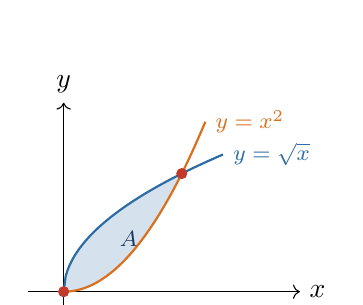
\begin{tikzpicture}[scale=1.5]
\draw[->] (-0.3,0)--(2.0,0) node[right]{$x$};
\draw[->] (0,-0.2)--(0,1.6) node[above]{$y$};
\fill[grafikMavi!20,domain=0:1,variable=\x]
  (0,0) -- plot ({\x},{sqrt(\x)}) -- (1,1) -- plot[domain=1:0] ({\x},{\x*\x}) -- cycle;
\draw[grafikMavi,thick,domain=0:1.35,samples=80] plot (\x,{sqrt(\x)}) node[right]{\footnotesize $y=\sqrt{x}$};
\draw[turuncu,thick,domain=0:1.2,samples=80] plot (\x,{\x*\x}) node[right]{\footnotesize $y=x^2$};
\filldraw[kirmizi] (0,0) circle (1.2pt);
\filldraw[kirmizi] (1,1) circle (1.2pt);
\node[anaMavi] at (0.55,0.45) {\footnotesize $A$};
\end{tikzpicture}
\end{center}

\soru{$y=x^2$ ve $y=\sqrt{x}$ eğrileri arasındaki alanı bulun.}

\cozum Kesişim: $x^2=\sqrt x\Rightarrow x=0,1$. $[0,1]$'de $\sqrt x\ge x^2$:
\[
A=\int_0^1\left(\sqrt x-x^2\right)dx=\left[\frac{2}{3}x^{3/2}-\frac{x^3}{3}\right]_0^1
=\frac23-\frac13=\frac13 .
\]

\pykontrol
\begin{lstlisting}
import sympy as sp
x = sp.symbols('x')

f, g = sp.sqrt(x), x**2
kesisim = sp.solve(sp.Eq(f, g), x)             # [0, 1]
A = sp.integrate(f - g, (x, 0, 1))             # 1/3
\end{lstlisting}

\begin{lstlisting}
import numpy as np, matplotlib.pyplot as plt

xs = np.linspace(0, 1, 300)
plt.plot(xs, np.sqrt(xs), lw=2, label=r'$y=\sqrt{x}$')
plt.plot(xs, xs**2, lw=2, label=r'$y=x^2$')
plt.fill_between(xs, xs**2, np.sqrt(xs), alpha=0.3)
plt.legend(); plt.grid(alpha=0.3); plt.title('Alan = 1/3'); plt.show()
\end{lstlisting}

\uyari{Eğriler aralıkta yer değiştiriyorsa (kesişim noktaları arada kalıyorsa)
integrali \emph{parçalara ayır} veya mutlak değerle hesapla; aksi hâlde
alanlar birbirini götürür.}

\begin{lstlisting}
# Kesisimlerde parcalara ayirarak guvenli alan hesabi
def egriler_arasi_alan(f, g, a, b, x=x):
    kesisimler = [k for k in sp.solve(sp.Eq(f, g), x)
                  if k.is_real and a < k < b]
    noktalar = [a] + sorted(kesisimler) + [b]
    toplam = 0
    for u, v in zip(noktalar[:-1], noktalar[1:]):
        toplam += abs(sp.integrate(f - g, (x, u, v)))
    return sp.simplify(toplam)

egriler_arasi_alan(sp.sin(x), sp.cos(x), 0, sp.pi)     # 2*sqrt(2)
\end{lstlisting}

% =====================================================================
\gsec{Dönel Hacim (Volume of Revolution)}
% =====================================================================

\gsub{Disk ve Halka (Washer) Yöntemi}

\kural{$x$ ekseni etrafında döndürme:
\[
V=\pi\int_a^b \bigl[f(x)\bigr]^2 dx \quad\text{(disk)},\qquad
V=\pi\int_a^b\Bigl(\bigl[R(x)\bigr]^2-\bigl[r(x)\bigr]^2\Bigr)dx \quad\text{(halka)} .
\]
$R$ dış yarıçap, $r$ iç yarıçaptır; ikisi de dönme eksenine olan uzaklıktır.}

\begin{center}
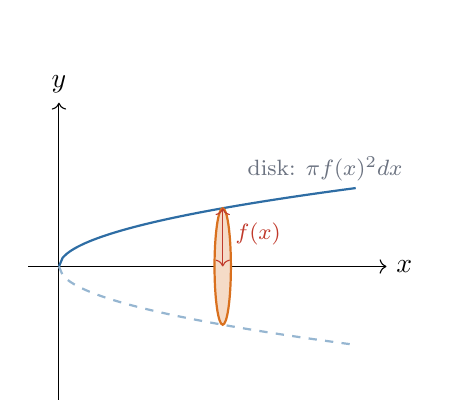
\begin{tikzpicture}[scale=1.3]
\draw[->] (-0.3,0)--(3.2,0) node[right]{$x$};
\draw[->] (0,-1.4)--(0,1.6) node[above]{$y$};
\draw[grafikMavi,thick,domain=0:2.9,samples=80] plot (\x,{0.45*sqrt(\x)});
\draw[grafikMavi!50,thick,dashed,domain=0:2.9,samples=80] plot (\x,{-0.45*sqrt(\x)});
\fill[turuncu!25] (1.6,0) ellipse (0.08 and 0.569);
\draw[turuncu,thick] (1.6,0) ellipse (0.08 and 0.569);
\draw[<->,kirmizi] (1.6,0)--(1.6,0.569);
\node[kirmizi,right] at (1.63,0.32) {\footnotesize $f(x)$};
\node[ortaGri] at (2.6,0.95) {\footnotesize disk: $\pi f(x)^2 dx$};
\end{tikzpicture}
\end{center}

\soru{$y=\sqrt{x}$, $y=0$, $x=4$ bölgesinin $x$ ekseni etrafında döndürülmesiyle
oluşan hacmi bulun.}

\cozum
\[
V=\pi\int_0^4\bigl(\sqrt x\bigr)^2dx=\pi\int_0^4 x\,dx=\pi\left[\frac{x^2}{2}\right]_0^4=8\pi .
\]

\pykontrol
\begin{lstlisting}
V = sp.pi*sp.integrate(sp.sqrt(x)**2, (x, 0, 4))     # 8*pi
float(V)                                              # 25.132741228718345
\end{lstlisting}

\soru{$y=x$ ve $y=x^2$ arasındaki bölge $x$ ekseni etrafında döndürülüyor.
Hacmi bulun.}

\cozum $[0,1]$'de $x\ge x^2$; dış yarıçap $R=x$, iç yarıçap $r=x^2$:
\[
V=\pi\int_0^1\left(x^2-x^4\right)dx=\pi\left(\frac13-\frac15\right)=\frac{2\pi}{15}.
\]

\begin{lstlisting}
V = sp.pi*sp.integrate(x**2 - x**4, (x, 0, 1))       # 2*pi/15
\end{lstlisting}

\gsub{Silindirik Kabuk Yöntemi (Cylindrical Shells)}

\kural{$y$ ekseni etrafında döndürmede kabuk yöntemi:
\[
V=2\pi\int_a^b x\,f(x)\dd x
\]
Genel hâli: $V=2\pi\int (\text{yarıçap})\times(\text{yükseklik})\,d(\text{kalınlık})$.}

\ipucu{Hangi yöntem? Dönme ekseni ile \emph{aynı} değişkende integral alıyorsan
kabuk, \emph{dik} değişkende integral alıyorsan disk/halka kullan. $y$ ekseni
etrafında dönen ve $y=f(x)$ olarak verilen bölgelerde kabuk genelde daha
kolaydır (ters fonksiyon bulmaya gerek kalmaz).}

\soru{$y=x^2$, $y=0$, $x=2$ bölgesi $y$ ekseni etrafında döndürülüyor. Hacmi
kabuk yöntemiyle bulun.}

\cozum
\[
V=2\pi\int_0^2 x\cdot x^2dx=2\pi\left[\frac{x^4}{4}\right]_0^2=8\pi .
\]

\begin{lstlisting}
V_kabuk = 2*sp.pi*sp.integrate(x*x**2, (x, 0, 2))    # 8*pi

# Ayni hacim disk yontemiyle (y'ye gore): x = sqrt(y), 0<=y<=4
y = sp.symbols('y')
V_disk = sp.pi*sp.integrate(2**2 - (sp.sqrt(y))**2, (y, 0, 4))   # 8*pi
\end{lstlisting}

\gsub{Kesit Alanıyla Hacim}

\kural{Dönel olmayan katılarda, $x$'e dik kesitin alanı $A(x)$ ise
\[ V=\int_a^b A(x)\dd x . \]}

\ornek{Tabanı $x^2+y^2\le1$ dairesi olan ve $x$ eksenine dik kesitleri kare
olan katının hacmi: kenar $2\sqrt{1-x^2}$, alan $A(x)=4(1-x^2)$;
$V=\int_{-1}^{1}4(1-x^2)dx=\frac{16}{3}$.}

\begin{lstlisting}
sp.integrate(4*(1 - x**2), (x, -1, 1))     # 16/3
\end{lstlisting}

% =====================================================================
\gsec{Yay Uzunluğu ve Dönel Yüzey Alanı}
% =====================================================================

\gsub{Yay Uzunluğu (Arc Length)}

\kural{
\[
L=\int_a^b\sqrt{1+\bigl[f'(x)\bigr]^2}\;dx
\qquad\text{veya}\qquad
L=\int_c^d\sqrt{1+\bigl[g'(y)\bigr]^2}\;dy .
\]}

Formülün kaynağı Pisagor'dur: $ds=\sqrt{dx^2+dy^2}=\sqrt{1+(dy/dx)^2}\,dx$.

\soru{$y=\dfrac{2}{3}x^{3/2}$ eğrisinin $[0,3]$ aralığındaki uzunluğunu bulun.}

\cozum $y'=x^{1/2}$, $1+(y')^2=1+x$:
\[
L=\int_0^3\sqrt{1+x}\,dx=\left[\frac23(1+x)^{3/2}\right]_0^3=\frac23(8-1)=\frac{14}{3}.
\]

\pykontrol
\begin{lstlisting}
f = sp.Rational(2,3)*x**sp.Rational(3,2)
L = sp.integrate(sp.sqrt(1 + sp.diff(f, x)**2), (x, 0, 3))    # 14/3
\end{lstlisting}

\begin{lstlisting}
# Genel yay uzunlugu fonksiyonu (sembolik + sayisal yedek)
from scipy.integrate import quad
import numpy as np

def yay_uzunlugu(f, a, b, x=x):
    integrand = sp.sqrt(1 + sp.diff(f, x)**2)
    try:
        sonuc = sp.integrate(integrand, (x, a, b))
        if sonuc.has(sp.Integral):
            raise ValueError
        return sp.simplify(sonuc)
    except Exception:
        g = sp.lambdify(x, integrand, 'numpy')
        return quad(g, float(a), float(b))[0]

yay_uzunlugu(sp.sin(x), 0, sp.pi)      # 3.8201977890277... (eliptik integral)
\end{lstlisting}

\gsub{Dönel Yüzey Alanı (Surface of Revolution)}

\kural{$x$ ekseni etrafında: $\displaystyle S=2\pi\int_a^b f(x)\sqrt{1+[f'(x)]^2}\,dx$.\\
$y$ ekseni etrafında: $\displaystyle S=2\pi\int_a^b x\sqrt{1+[f'(x)]^2}\,dx$.}

\soru{$y=\sqrt{x}$, $1\le x\le4$ eğrisinin $x$ ekseni etrafında döndürülmesiyle
oluşan yüzeyin alanını bulun.}

\cozum $y'=\frac{1}{2\sqrt x}$, $1+(y')^2=\frac{4x+1}{4x}$:
\[
S=2\pi\int_1^4\sqrt x\cdot\frac{\sqrt{4x+1}}{2\sqrt x}dx
=\pi\int_1^4\sqrt{4x+1}\,dx=\frac{\pi}{6}\left(17^{3/2}-5^{3/2}\right).
\]

\begin{lstlisting}
f = sp.sqrt(x)
S = 2*sp.pi*sp.integrate(f*sp.sqrt(1 + sp.diff(f, x)**2), (x, 1, 4))
sp.simplify(S)        # pi*(-5*sqrt(5) + 17*sqrt(17))/6
float(S)              # 30.846...
\end{lstlisting}

\ornek[Küre Kontrolü]{$f(x)=\sqrt{r^2-x^2}$, $[-r,r]$ için
$S=2\pi\int_{-r}^{r}\sqrt{r^2-x^2}\cdot\frac{r}{\sqrt{r^2-x^2}}dx=4\pi r^2$
--- kürenin yüzey alanı formülü.}

% =====================================================================
\gsec{Fizik Uygulamaları: İş, Basınç, Kütle Merkezi}
% =====================================================================

\gsub{İş (Work)}

\kural{Değişken kuvvet altında iş: $\displaystyle W=\int_a^b F(x)\dd x$.\\
Hooke yasası: $F(x)=kx$ (yay). Pompalama: $W=\int \rho g\,A(y)\,d(y)\times$
(taşınacak yükseklik).}

\soru{Doğal boyu $10$ cm olan bir yayı $2$ cm germek için $40$ J iş
gerekiyorsa, $5$ cm germek için ne kadar iş gerekir?}

\cozum $W=\int_0^{0.02}kx\,dx=\frac{k(0.02)^2}{2}=40\Rightarrow k=200000$ N/m.
$W_5=\frac{k(0.05)^2}{2}=250$ J.

\begin{lstlisting}
k = sp.symbols('k', positive=True)
W = sp.integrate(k*x, (x, 0, 0.02))
k_deger = sp.solve(sp.Eq(W, 40), k)[0]           # 200000
sp.integrate(k_deger*x, (x, 0, 0.05))            # 250
\end{lstlisting}

\soru{Yüksekliği $10$ m, yarıçapı $3$ m olan silindirik bir tank su doludur.
Suyun tamamını tankın üstünden dışarı pompalamak için gereken işi bulun.
($\rho=1000$ kg/m$^3$, $g=9.8$)}

\cozum $y$ derinliğindeki ince dilim: hacim $\pi r^2dy$, ağırlık
$\rho g\pi r^2 dy$, taşınacak yükseklik $(10-y)$:
\[
W=\int_0^{10}1000\cdot9.8\cdot\pi\cdot9\,(10-y)\,dy = 9.8\cdot9000\pi\cdot50
\approx 1.385\times10^{7}\ \text{J}.
\]

\begin{lstlisting}
y = sp.symbols('y')
rho, g, r = 1000, 9.8, 3
W = sp.integrate(rho*g*sp.pi*r**2*(10 - y), (y, 0, 10))
float(W)          # 13854423.6...
\end{lstlisting}

\gsub{Kütle Merkezi (Centroid)}

\kural{Yoğunluğu sabit, $y=f(x)$ ile $x$ ekseni arasındaki bölgenin ağırlık
merkezi:
\[
\bar{x}=\frac{1}{A}\int_a^b x f(x)\dd x,\qquad
\bar{y}=\frac{1}{A}\int_a^b \frac{\bigl[f(x)\bigr]^2}{2}\dd x,\qquad
A=\int_a^b f(x)\dd x .
\]}

\soru{$y=x^2$, $x\in[0,1]$ ile $x$ ekseni arasındaki bölgenin ağırlık merkezini
bulun.}

\cozum $A=\frac13$. $\bar x=3\int_0^1x^3dx=\frac34$;
$\bar y=3\int_0^1\frac{x^4}{2}dx=\frac{3}{10}$.

\begin{lstlisting}
f = x**2
A  = sp.integrate(f, (x, 0, 1))                       # 1/3
xb = sp.integrate(x*f, (x, 0, 1))/A                   # 3/4
yb = sp.integrate(f**2/2, (x, 0, 1))/A                # 3/10
print(xb, yb)
\end{lstlisting}

\notk[Pappus Teoremi]{Bir bölge, kendisini kesmeyen bir eksen etrafında
döndürülürse oluşan cismin hacmi $V=2\pi\bar{r}A$'dır; burada $\bar r$ ağırlık
merkezinin eksene uzaklığı, $A$ bölgenin alanıdır. Kabuk yönteminin şık bir
özetidir.}

\gsub{Olasılık Yoğunluk Fonksiyonu}

\kural{$f$ bir olasılık yoğunluk fonksiyonuysa (pdf):
\[
f(x)\ge0,\qquad \int_{-\infty}^{\infty}f(x)\dd x=1,\qquad
P(a\le X\le b)=\int_a^b f(x)\dd x,
\]
beklenen değer $\mu=\int_{-\infty}^{\infty}x f(x)\dd x$.}

\ornek{Üstel dağılım $f(x)=\lambda e^{-\lambda x}$, $x\ge0$:
$\int_0^{\infty}\lambda e^{-\lambda x}dx=1$ ve $\mu=\frac{1}{\lambda}$.}

\begin{lstlisting}
lam = sp.symbols('lambda', positive=True)
f = lam*sp.exp(-lam*x)

sp.integrate(f, (x, 0, sp.oo))          # 1
sp.integrate(x*f, (x, 0, sp.oo))        # 1/lambda      (ortalama)
sp.integrate(x**2*f, (x, 0, sp.oo))     # 2/lambda**2   (ikinci moment)
\end{lstlisting}

% =====================================================================
\gsec{Ekonomi ve Biyolojide İntegral}
% =====================================================================

\gsub{Tüketici ve Üretici Artığı}

\kural{$p(x)$ talep fonksiyonu, $P=p(Q)$ piyasa fiyatı olsun.
\[
\text{Tüketici artığı}=\int_0^{Q}\bigl(p(x)-P\bigr)\dd x,
\qquad
\text{Üretici artığı}=\int_0^{Q}\bigl(P-p_{\text{arz}}(x)\bigr)\dd x .
\]
Tüketici artığı, ``ödemeye razı olunan'' ile ``gerçekte ödenen'' arasındaki
farkın toplamıdır --- talep eğrisi ile fiyat doğrusu arasındaki alan.}

\soru{Talep fonksiyonu $p(x)=50-0{,}05x$ TL ve piyasa fiyatı $P=20$ TL ise
tüketici artığını bulun.}

\cozum Önce $Q$: $50-0{,}05Q=20 \Rightarrow Q=600$.
\[
\int_0^{600}\bigl(50-0{,}05x-20\bigr)dx
=\Bigl[30x-0{,}025x^2\Bigr]_0^{600}=18000-9000=9000\ \text{TL}.
\]

\pykontrol
\begin{lstlisting}
import sympy as sp
x = sp.symbols('x')

p = 50 - sp.Rational(5,100)*x
Q = sp.solve(sp.Eq(p, 20), x)[0]            # 600
sp.integrate(p - 20, (x, 0, Q))             # 9000
\end{lstlisting}

\gsub{Kan Akışı ve Kardiyak Debi}

\kural[Poiseuille Yasası]{Yarıçapı $R$ olan bir damarda, merkezden $r$
uzaklıktaki hız $v(r)=\dfrac{P}{4\eta l}\bigl(R^2-r^2\bigr)$'dir. Toplam akış
(debi), ince halkaların katkısı toplanarak bulunur:
\[
F=\int_0^{R} 2\pi r\,v(r)\dd r=\frac{\pi P R^4}{8\eta l}.
\]}

Sonuçtaki $R^4$ çarpanı çarpıcıdır: damar yarıçapı yalnızca $\%10$ daralırsa
akış $\%34$ azalır --- tıptaki damar tıkanıklığının neden bu kadar kritik
olduğunun kalkülüs açıklaması.

\begin{lstlisting}
r, R, P, eta, l = sp.symbols('r R P eta l', positive=True)

v = P/(4*eta*l)*(R**2 - r**2)
F = sp.integrate(2*sp.pi*r*v, (r, 0, R))
sp.simplify(F)                 # pi*P*R**4/(8*eta*l)

# Yaricap %10 azalirsa akis orani
float(sp.Rational(9,10)**4)    # 0.6561  -> akis %34 azalir
\end{lstlisting}

\ornek[Kardiyak Debi]{Boya seyreltme yönteminde $t$ anındaki boya
derişimi $c(t)$ ölçülür; kalbin dakikadaki kan debisi
$F=\dfrac{A}{\int_0^{T}c(t)\dd t}$ ile bulunur ($A$: enjekte edilen boya
miktarı). Payda, ölçüm eğrisinin altındaki alandır ve pratikte Simpson
kuralıyla hesaplanır.}

\gsub{Birikim ve Ortalama: Genel Kural}

\ipucu{Bu bölümdeki bütün formüller tek bir fikrin kılığa girmiş hâlidir:
\emph{küçük bir dilimin katkısını yaz, integralle topla}. İş için
$dW=F\dd x$, hacim için $dV=A(x)\dd x$, akış için $dF=2\pi r v(r)\dd r$,
artık için $d(\text{artık})=(p(x)-P)\dd x$. Yeni bir uygulamayla
karşılaştığında yapman gereken tek şey ``bir dilimin katkısı nedir?''
sorusunu cevaplamaktır.}

% #####################################################################
\gpart{7}{Calculus 2 --- Diferansiyel Denklemlere Giriş}
% #####################################################################

% =====================================================================
\gsec{Temel Kavramlar ve Yön Alanları}
% =====================================================================

\tanim{Bilinmeyeni bir \emph{fonksiyon} olan ve bu fonksiyonun türevlerini
içeren denkleme \emph{diferansiyel denklem} denir. En yüksek türev mertebesi
denklemin mertebesidir. $y'=f(x,y)$ birinci mertebeden bir denklemdir.}

\ornek{$y'=ky$ (üstel büyüme), $y''+\omega^2y=0$ (harmonik salınım),
$y'=k y(M-y)$ (lojistik büyüme) --- doğa yasalarının çoğu diferansiyel
denklemdir.}

\gsub{Yön Alanı (Slope Field)}

$y'=f(x,y)$ denklemi, düzlemin her noktasında çözüm eğrisinin eğimini söyler.
Bu eğimleri kısa çizgilerle çizersek çözümlerin ``akışını'' görürüz.

\begin{lstlisting}
import numpy as np, matplotlib.pyplot as plt

def yon_alani(f, xr=(-3, 3), yr=(-3, 3), n=20):
    """y' = f(x, y) icin yon alani cizer."""
    X, Y = np.meshgrid(np.linspace(*xr, n), np.linspace(*yr, n))
    U = np.ones_like(X)
    V = f(X, Y)
    N = np.hypot(U, V)                 # birim uzunluga normalize et
    plt.quiver(X, Y, U/N, V/N, color='#6B7280', angles='xy')
    plt.grid(alpha=0.25)

yon_alani(lambda X, Y: Y*(1 - Y))      # lojistik denklem
# Uzerine bir cozum egrisi
from scipy.integrate import solve_ivp
s = solve_ivp(lambda t, y: y*(1 - y), [-3, 3], [0.1], dense_output=True)
ts = np.linspace(-3, 3, 300)
plt.plot(ts, s.sol(ts)[0], lw=2, color='#D9701E')
plt.show()
\end{lstlisting}

% =====================================================================
\gsec{Ayrılabilir Değişkenli Denklemler (Separable)}
% =====================================================================

\kural{$\dfrac{dy}{dx}=g(x)h(y)$ biçimindeki denklemde değişkenleri ayır:
\[
\int\frac{dy}{h(y)}=\int g(x)\dd x .
\]}

\soru{$\dfrac{dy}{dx}=\dfrac{x}{y}$, $y(0)=2$ başlangıç değer problemini
çözün.}

\cozum $y\,dy=x\,dx \Rightarrow \frac{y^2}{2}=\frac{x^2}{2}+C
\Rightarrow y^2=x^2+C_1$. $y(0)=2$: $4=C_1$. Çözüm: $y=\sqrt{x^2+4}$.

\pykontrol
\begin{lstlisting}
import sympy as sp
x = sp.symbols('x')
y = sp.Function('y')

ode = sp.Eq(y(x).diff(x), x/y(x))
sp.dsolve(ode)                                  # y(x) = +-sqrt(C1 + x**2)
sp.dsolve(ode, ics={y(0): 2})                   # y(x) = sqrt(x**2 + 4)
\end{lstlisting}

\gsub{Üstel Büyüme ve Azalma}

\kural{$\dfrac{dy}{dt}=ky \Rightarrow y(t)=y_0e^{kt}$. $k>0$ büyüme, $k<0$
azalmadır. Yarı ömür: $t_{1/2}=\dfrac{\ln 2}{|k|}$.}

\soru{Bir radyoaktif maddenin yarı ömrü $30$ yıldır. $100$ gramdan $100$ yıl
sonra ne kadar kalır?}

\cozum $k=-\frac{\ln2}{30}$. $y(100)=100e^{-100\ln2/30}=100\cdot2^{-10/3}
\approx9.92$ g.

\begin{lstlisting}
t = sp.symbols('t', positive=True)
k = -sp.log(2)/30
y_t = 100*sp.exp(k*t)
float(y_t.subs(t, 100))          # 9.921256574801247
\end{lstlisting}

% =====================================================================
\gsec{Birinci Mertebe Lineer Denklemler}
% =====================================================================

\kural{$y'+P(x)y=Q(x)$ denklemi için \emph{integral çarpanı}
$\mu(x)=e^{\int P(x)dx}$ ile çarparız; sol taraf $(\mu y)'$ olur:
\[
y=\frac{1}{\mu(x)}\left(\int \mu(x)Q(x)\dd x + C\right).
\]}

\soru{$y'+2y=e^{-x}$ denklemini çözün.}

\cozum $\mu=e^{2x}$. $(e^{2x}y)'=e^{x}$, yani $e^{2x}y=e^x+C$:
\[ y=e^{-x}+Ce^{-2x}. \]

\pykontrol
\begin{lstlisting}
ode = sp.Eq(y(x).diff(x) + 2*y(x), sp.exp(-x))
sp.dsolve(ode)                    # y(x) = (C1 + exp(x))*exp(-2*x)
sp.classify_ode(ode)              # ('1st_linear', 'nth_linear_...', ...)
\end{lstlisting}

\ipucu{\code{sp.classify\_ode(ode)} bir denklemin \emph{hangi tipte} olduğunu
söyler: ayrılabilir mi, lineer mi, tam mı, homojen mi. Elle çözmeden önce
yöntem seçmek için mükemmel bir kontrol aracıdır.}

% =====================================================================
\gsec{Sayısal Çözüm: Euler Yöntemi ve solve\_ivp}
% =====================================================================

Çoğu diferansiyel denklemin kapalı çözümü yoktur; sayısal olarak çözeriz.

\kural[Euler Yöntemi]{$y'=f(x,y)$, $y(x_0)=y_0$ için
\[
y_{n+1}=y_n+h\,f(x_n,y_n),\qquad x_{n+1}=x_n+h .
\]
Yerel hata $O(h^2)$, toplam hata $O(h)$'dir.}

\begin{lstlisting}
import numpy as np

def euler(f, x0, y0, xson, h=0.1):
    xs, ys = [x0], [y0]
    while xs[-1] < xson - 1e-12:
        ys.append(ys[-1] + h*f(xs[-1], ys[-1]))
        xs.append(xs[-1] + h)
    return np.array(xs), np.array(ys)

# y' = y, y(0) = 1  -> gercek cozum e^x
for h in [0.5, 0.1, 0.01]:
    xs, ys = euler(lambda t, y: y, 0, 1, 1, h)
    print(f"h={h:<5} y(1)={ys[-1]:.6f}  hata={abs(ys[-1]-np.e):.6f}")
\end{lstlisting}

\begin{lstlisting}[style=outstyle]
h=0.5   y(1)=2.250000  hata=0.468282
h=0.1   y(1)=2.593742  hata=0.124539
h=0.01  y(1)=2.704814  hata=0.013468
\end{lstlisting}

$h$ onda birine inince hata da onda birine iniyor: birinci mertebe yakınsama.

\begin{lstlisting}
# Profesyonel cozucu: adaptif Runge-Kutta
from scipy.integrate import solve_ivp
import numpy as np

sol = solve_ivp(lambda t, y: y, [0, 1], [1], rtol=1e-10, atol=1e-12)
print(sol.y[0, -1], np.e)        # 2.718281828... 2.718281828...
\end{lstlisting}

% =====================================================================
\gsec{Lojistik Büyüme ve Uygulama Modelleri}
% =====================================================================

\kural[Lojistik Denklem]{
\[
\frac{dP}{dt}=kP\left(1-\frac{P}{M}\right)
\quad\Longrightarrow\quad
P(t)=\frac{M}{1+Ae^{-kt}},\qquad A=\frac{M-P_0}{P_0}.
\]
$M$ taşıma kapasitesidir; $P\to M$ olur.}

\begin{lstlisting}
t = sp.symbols('t')
P = sp.Function('P')
k, M = sp.symbols('k M', positive=True)

ode = sp.Eq(P(t).diff(t), k*P(t)*(1 - P(t)/M))
sp.dsolve(ode, P(t))
# P(t) = M/(C1*M*exp(-k*t) + 1)  benzeri
\end{lstlisting}

\begin{lstlisting}
import numpy as np, matplotlib.pyplot as plt

M, k, P0 = 1000, 0.5, 10
A = (M - P0)/P0
ts = np.linspace(0, 25, 400)
Pt = M/(1 + A*np.exp(-k*ts))

plt.plot(ts, Pt, lw=2, color='#2E6DA4')
plt.axhline(M, ls='--', color='#C0392B', label='tasima kapasitesi M')
plt.xlabel('t'); plt.ylabel('P(t)'); plt.legend(); plt.grid(alpha=0.3); plt.show()
\end{lstlisting}

\ornek[Newton'un Soğuma Yasası]{$\dfrac{dT}{dt}=k(T-T_{\text{ortam}})$;
çözümü $T(t)=T_{\text{ortam}}+(T_0-T_{\text{ortam}})e^{kt}$. Ayrılabilir bir
denklemdir ve adli tıptan kahve soğutmaya kadar her yerde kullanılır.}

\begin{lstlisting}
T = sp.Function('T'); Ta, k = sp.symbols('T_a k')
ode = sp.Eq(T(t).diff(t), k*(T(t) - Ta))
sp.dsolve(ode, T(t))            # T(t) = C1*exp(k*t) + T_a
\end{lstlisting}

% =====================================================================
\gsec{Karışım Problemleri, Ortogonal Yörüngeler ve Sistemler}
% =====================================================================

\gsub{Karışım (Mixing) Problemleri}

\kural{Bir tanktaki çözünmüş madde miktarı $y(t)$ için
\[
\frac{dy}{dt}=(\text{giriş hızı})-(\text{çıkış hızı})
=r_{\text{gir}}c_{\text{gir}}-r_{\text{çık}}\frac{y}{V(t)} .
\]
Bu, birinci mertebe \emph{lineer} bir denklemdir; integral çarpanıyla çözülür.}

\soru{$1000$ L su içeren bir tanka, litresinde $0{,}1$ kg tuz bulunan çözelti
dakikada $10$ L girmekte; karışım aynı hızla çıkmaktadır. Başlangıçta tankta
tuz yoktur. $t$ dakika sonra tanktaki tuz miktarını bulun.}

\cozum Hacim sabit ($1000$ L). Giriş: $10\cdot0{,}1=1$ kg/dk. Çıkış:
$10\cdot\dfrac{y}{1000}=\dfrac{y}{100}$ kg/dk.
\[
y'=1-\frac{y}{100},\qquad y(0)=0
\quad\Longrightarrow\quad
y(t)=100\left(1-e^{-t/100}\right).
\]
$t\to\infty$ iken $y\to100$ kg; yani tank sonunda giriş derişimine
($0{,}1$ kg/L) ulaşır --- fiziksel olarak beklenen sonuç.

\pykontrol
\begin{lstlisting}
import sympy as sp
t = sp.symbols('t')
y = sp.Function('y')

ode = sp.Eq(y(t).diff(t), 1 - y(t)/100)
sp.dsolve(ode, y(t), ics={y(0): 0})
# Eq(y(t), 100 - 100*exp(-t/100))

sp.limit(100 - 100*sp.exp(-t/100), t, sp.oo)     # 100
\end{lstlisting}

\gsub{Ortogonal Yörüngeler}

Bir eğri ailesinin her üyesini dik kesen eğriler ailesine \emph{ortogonal
yörüngeler} denir. Fizikte eş potansiyel çizgileri ile alan çizgileri böyle
bir çifttir.

\kural{Yöntem: (1) Aileden $c$ sabitini eleyerek $y'=f(x,y)$ elde et.
(2) Eğimi ters işaretli tersiyle değiştir: $y'=-\dfrac{1}{f(x,y)}$.
(3) Yeni denklemi çöz.}

\soru{$y=cx^2$ parabol ailesinin ortogonal yörüngelerini bulun.}

\cozum $y'=2cx$ ve $c=y/x^2$ olduğundan $y'=\dfrac{2y}{x}$. Dikleşmek için
\[
y'=-\frac{x}{2y}
\;\Longrightarrow\;
2y\dd y=-x\dd x
\;\Longrightarrow\;
y^2+\frac{x^2}{2}=k .
\]
Yani ortogonal yörüngeler bir elips ailesidir.

\begin{lstlisting}
x, c = sp.symbols('x c')
y = sp.Function('y')

# Aile: y = c*x**2  ->  c = y/x**2  ->  y' = 2*c*x = 2*y/x
# Ortogonal egim: y' = -x/(2*y)
sp.dsolve(sp.Eq(y(x).diff(x), -x/(2*y(x))), y(x))
# y(x) = +-sqrt(C1 - x**2/2)   -> elips ailesi
\end{lstlisting}

\gsub{Diferansiyel Denklem Sistemleri: Av-Avcı Modeli}

İki tür birbirini etkiliyorsa tek denklem yetmez. \emph{Lotka--Volterra}
modeli, av ($R$) ve avcı ($W$) nüfuslarını birlikte tanımlar:
\[
\frac{dR}{dt}=aR-bRW,\qquad
\frac{dW}{dt}=-cW+dRW .
\]
Çözümler kapalı formda yazılamaz; sayısal olarak çözülür ve nüfuslar
\emph{periyodik} olarak salınır.

\begin{lstlisting}
import numpy as np, matplotlib.pyplot as plt
from scipy.integrate import solve_ivp

a, b, c, d = 1.0, 0.1, 1.5, 0.075

def av_avci(t, z):
    R, W = z
    return [a*R - b*R*W, -c*W + d*R*W]

sol = solve_ivp(av_avci, [0, 40], [40, 9], dense_output=True, rtol=1e-8)
ts = np.linspace(0, 40, 2000)
R, W = sol.sol(ts)

fig, (ax1, ax2) = plt.subplots(1, 2, figsize=(11, 4))
ax1.plot(ts, R, label='av (R)'); ax1.plot(ts, W, label='avci (W)')
ax1.set_xlabel('t'); ax1.legend(); ax1.grid(alpha=0.3)
ax2.plot(R, W, color='#D9701E')          # faz portresi: kapali egri
ax2.set_xlabel('R'); ax2.set_ylabel('W'); ax2.grid(alpha=0.3)
plt.tight_layout(); plt.show()
\end{lstlisting}

\bilgi{Faz portresinde (sağdaki grafik) kapalı bir eğri görürsün: nüfuslar
aynı döngüyü tekrar tekrar izler. Denge noktası $R=c/d$, $W=a/b$'dir ve
çözümler bu noktanın etrafında döner. İkinci mertebe denklemler de aynı
şekilde birinci mertebe sistemlere çevrilerek \code{solve\_ivp} ile çözülür:
$y''=f \Rightarrow z=(y,y')$.}

% #####################################################################
\gpart{8}{Calculus 2 --- Diziler ve Seriler}
% #####################################################################

% =====================================================================
\gsec{Diziler (Sequences)}
% =====================================================================

\tanim{Dizi, tanım kümesi doğal sayılar olan bir fonksiyondur:
$\{a_n\}_{n=1}^{\infty}$. $\lim_{n\to\infty}a_n=L$ sonluysa dizi
\emph{yakınsaktır}; aksi hâlde \emph{ıraksaktır}.}

\begin{center}
\renewcommand{\arraystretch}{2.4}
\begin{tabularx}{\textwidth}{@{}>{$\displaystyle}l<{$} X@{}}
\toprule
\rowcolor{acikMavi}\multicolumn{1}{@{}l}{\color{anaMavi}\textbf{Dizi}} & \multicolumn{1}{l@{}}{\color{anaMavi}\textbf{Davranış}}\\
\midrule
a_n=\frac{1}{n} & $0$'a yakınsar.\\
\rowcolor{acikGri} a_n=r^n & $|r|<1$ ise $0$; $r=1$ ise $1$; diğer hâllerde ıraksar.\\
a_n=\left(1+\frac{1}{n}\right)^n & $e$'ye yakınsar.\\
\rowcolor{acikGri} a_n=\frac{n!}{n^n} & $0$'a yakınsar ($n^n$ çok daha hızlı büyür).\\
a_n=(-1)^n & Iraksar (salınır).\\
\rowcolor{acikGri} a_n=\sqrt[n]{n} & $1$'e yakınsar.\\
\bottomrule
\end{tabularx}
\end{center}

\teorem[Monoton Yakınsaklık]{Artan ve üstten sınırlı (ya da azalan ve alttan
sınırlı) her dizi yakınsaktır.}

\teorem[Sıkıştırma]{$b_n\le a_n\le c_n$ ve $\lim b_n=\lim c_n=L$ ise
$\lim a_n=L$. Ayrıca $\lim|a_n|=0 \Rightarrow \lim a_n=0$.}

\begin{lstlisting}
import sympy as sp
n = sp.symbols('n', positive=True, integer=True)

sp.limit(1/n, n, sp.oo)                    # 0
sp.limit((1 + 1/n)**n, n, sp.oo)           # E
sp.limit(sp.factorial(n)/n**n, n, sp.oo)   # 0
sp.limit(n**(1/n), n, sp.oo)               # 1
sp.limit(sp.log(n)/n, n, sp.oo)            # 0
\end{lstlisting}

\begin{lstlisting}
import numpy as np, matplotlib.pyplot as plt

ns = np.arange(1, 31)
plt.stem(ns, (1 + 1/ns)**ns)
plt.axhline(np.e, ls='--', color='#C0392B', label='e')
plt.xlabel('n'); plt.legend(); plt.grid(alpha=0.3); plt.show()
\end{lstlisting}

\bilgi{Büyüme hızı sıralaması (en yavaştan en hızlıya):
\[
\ln n \prec n^p \prec a^n \prec n! \prec n^n .
\]
Bu sıralama hem dizi limitlerinde hem de seri testlerinde sürekli işine
yarayacak.}

% =====================================================================
\gsec{Seriler ve Kısmi Toplamlar}
% =====================================================================

\tanim{$\displaystyle\sum_{n=1}^{\infty}a_n$ serisinin $n$. kısmi toplamı
$s_n=a_1+a_2+\dots+a_n$'dir. $\lim_{n\to\infty}s_n=S$ sonluysa seri
\emph{yakınsaktır} ve toplamı $S$'dir.}

\gsub{Geometrik Seri}

\kural{
\[
\sum_{n=0}^{\infty}ar^n=a+ar+ar^2+\dots=
\begin{cases}
\dfrac{a}{1-r}, & |r|<1 \quad\text{(yakınsak)}\\[6pt]
\text{ıraksak}, & |r|\ge1
\end{cases}
\]
Kısmi toplam: $s_n=a\dfrac{1-r^n}{1-r}$.}

\soru{$\displaystyle\sum_{n=1}^{\infty}\frac{3}{2^n}$ serisinin toplamını
bulun.}

\cozum İlk terim $a=\frac32$, oran $r=\frac12$:
$S=\dfrac{3/2}{1-1/2}=3$.

\pykontrol
\begin{lstlisting}
sp.summation(3/2**n, (n, 1, sp.oo))          # 3
sp.summation(sp.Rational(1,2)**n, (n, 0, sp.oo))   # 2

# Kismi toplamlarla sayisal dogrulama
import numpy as np
ks = np.arange(1, 21)
print(np.cumsum(3/2.0**ks)[-5:])     # 2.99997... -> 3
\end{lstlisting}

\gsub{Teleskopik Seri}

Terimler birbirini götürür; kısmi toplamı doğrudan yazılır.

\soru{$\displaystyle\sum_{n=1}^{\infty}\frac{1}{n(n+1)}$ toplamını bulun.}

\cozum $\frac{1}{n(n+1)}=\frac1n-\frac{1}{n+1}$. Kısmi toplam
$s_n=1-\frac{1}{n+1}\to1$. Toplam $=1$.

\begin{lstlisting}
sp.apart(1/(n*(n + 1)))                        # -1/(n + 1) + 1/n
sp.summation(1/(n*(n + 1)), (n, 1, sp.oo))     # 1
\end{lstlisting}

\gsub{Iraksaklık Testi (n. Terim Testi)}

\kural{$\displaystyle\lim_{n\to\infty}a_n\neq0$ ise $\sum a_n$ \textbf{ıraksar}.
Ancak $\lim a_n=0$ olması yakınsaklık için \emph{yeterli değildir}
(karşı örnek: harmonik seri).}

\uyari{Bu testin tek yönlü olduğunu unutma. ``Terimler sıfıra gidiyor, öyleyse
seri yakınsar'' \textbf{yanlıştır}. $\sum\frac1n$ ıraksar ama terimleri
sıfıra gider.}

\gsub{Harmonik Seri ve $p$-Serisi}

\kural{
\[
\sum_{n=1}^{\infty}\frac{1}{n^p}=
\begin{cases}\text{yakınsak}, & p>1\\ \text{ıraksak}, & p\le1\end{cases}
\]
$p=1$ hâli \emph{harmonik seridir} ve ıraksar (çok yavaş: ilk milyon terimin
toplamı yalnızca $\approx14.4$).}

\begin{lstlisting}
sp.summation(1/n**2, (n, 1, sp.oo))     # pi**2/6      (Basel problemi)
sp.summation(1/n**3, (n, 1, sp.oo))     # zeta(3)
sp.summation(1/n, (n, 1, sp.oo))        # oo

import numpy as np
N = 10**6
print(np.sum(1.0/np.arange(1, N + 1)))  # 14.392726722865724
\end{lstlisting}

% =====================================================================
\gsec{Yakınsaklık Testleri}
% =====================================================================

\gsub{İntegral Testi}

\teorem{$f$ pozitif, sürekli ve azalan bir fonksiyon, $a_n=f(n)$ olsun.
$\displaystyle\sum a_n$ ile $\displaystyle\int_1^{\infty}f(x)\dd x$ aynı anda
yakınsar veya ıraksar.}

\soru{$\displaystyle\sum_{n=2}^{\infty}\frac{1}{n\ln n}$ serisini inceleyin.}

\cozum $f(x)=\frac{1}{x\ln x}$ pozitif ve azalan.
$\int_2^{\infty}\frac{dx}{x\ln x}=[\ln(\ln x)]_2^{\infty}=\infty$: seri
\textbf{ıraksar}.

\begin{lstlisting}
x = sp.symbols('x', positive=True)
sp.integrate(1/(x*sp.log(x)), (x, 2, sp.oo))     # oo  -> iraksak
sp.integrate(1/(x*sp.log(x)**2), (x, 2, sp.oo))  # 1/log(2)  -> yakinsak
\end{lstlisting}

\gsub{Karşılaştırma Testleri}

\teorem[Doğrudan Karşılaştırma]{$0\le a_n\le b_n$ olsun.
$\sum b_n$ yakınsaksa $\sum a_n$ yakınsar; $\sum a_n$ ıraksaksa $\sum b_n$
ıraksar.}

\teorem[Limit Karşılaştırma]{$a_n,b_n>0$ ve
$\displaystyle\lim_{n\to\infty}\frac{a_n}{b_n}=c$ sonlu ve pozitifse, iki seri
\emph{aynı} davranışı gösterir. Karşılaştırma serisi olarak genelde $p$-serisi
veya geometrik seri seçilir.}

\soru{$\displaystyle\sum_{n=1}^{\infty}\frac{2n^2+3n}{n^4+5}$ serisini
inceleyin.}

\cozum Baskın terimler: $\frac{2n^2}{n^4}=\frac{2}{n^2}$. $b_n=\frac{1}{n^2}$
alalım: $\lim\frac{a_n}{b_n}=2$ (sonlu, pozitif). $\sum\frac1{n^2}$ yakınsak
($p=2>1$) olduğundan seri \textbf{yakınsaktır}.

\begin{lstlisting}
a = (2*n**2 + 3*n)/(n**4 + 5)
b = 1/n**2
sp.limit(a/b, n, sp.oo)                   # 2   -> ayni davranis
sp.summation(a, (n, 1, sp.oo)).evalf()    # sonlu bir sayi
\end{lstlisting}

\gsub{Oran Testi (Ratio Test)}

\teorem{$\displaystyle L=\lim_{n\to\infty}\left|\frac{a_{n+1}}{a_n}\right|$
olsun.
\begin{itemize}\itemsep1pt
\item $L<1$: seri \emph{mutlak yakınsaktır}.
\item $L>1$ (veya $\infty$): seri ıraksar.
\item $L=1$: test sonuçsuzdur, başka test dene.
\end{itemize}}

Faktöriyel ve $r^n$ içeren serilerde ilk tercih budur.

\soru{$\displaystyle\sum_{n=1}^{\infty}\frac{2^n}{n!}$ serisini inceleyin.}

\cozum
\[
\frac{a_{n+1}}{a_n}=\frac{2^{n+1}}{(n+1)!}\cdot\frac{n!}{2^n}=\frac{2}{n+1}\to0<1 .
\]
Seri yakınsaktır (toplamı $e^2-1$).

\pykontrol
\begin{lstlisting}
a = 2**n/sp.factorial(n)
oran = sp.simplify(a.subs(n, n + 1)/a)      # 2/(n + 1)
sp.limit(oran, n, sp.oo)                     # 0   -> yakinsak
sp.summation(a, (n, 1, sp.oo))               # -1 + exp(2)
\end{lstlisting}

\begin{lstlisting}
def oran_testi(a_n, n=n):
    """Oran testini uygular ve karari yazdirir."""
    L = sp.limit(sp.Abs(a_n.subs(n, n + 1)/a_n), n, sp.oo)
    karar = ("mutlak yakinsak" if L < 1 else
             "iraksak" if L > 1 else "sonucsuz (L = 1)")
    print(f"L = {L}  ->  {karar}")
    return L

oran_testi(2**n/sp.factorial(n))       # L = 0  -> mutlak yakinsak
oran_testi(1/n**2)                     # L = 1  -> sonucsuz
oran_testi(sp.factorial(n)/2**n)       # L = oo -> iraksak
\end{lstlisting}

\gsub{Kök Testi (Root Test)}

\teorem{$L=\displaystyle\lim_{n\to\infty}\sqrt[n]{|a_n|}$ olsun. $L<1$
yakınsak, $L>1$ ıraksak, $L=1$ sonuçsuz.}

Terimlerin tamamı $n$. kuvvetteyse ($a_n=(\dots)^n$) bu test çok pratiktir.

\begin{lstlisting}
a = (n/(2*n + 1))**n
sp.limit(sp.root(sp.Abs(a), n), n, sp.oo)     # 1/2  -> yakinsak
\end{lstlisting}

\gsub{Alterne Seri Testi (Leibniz)}

\teorem{$\displaystyle\sum(-1)^{n-1}b_n$ serisinde $b_n>0$ olsun. Eğer
(i) $b_{n+1}\le b_n$ (azalan) ve (ii) $\lim b_n=0$ ise seri yakınsaktır.
Ayrıca kalan hatası ilk ihmal edilen terimden küçüktür:
$|S-s_n|\le b_{n+1}$.}

\soru{$\displaystyle\sum_{n=1}^{\infty}\frac{(-1)^{n-1}}{n}$ (alterne harmonik)
serisini inceleyin ve toplamını $0.01$ hassasiyetle veren terim sayısını bulun.}

\cozum $b_n=\frac1n$ azalan ve $0$'a gidiyor: yakınsak (toplamı $\ln2$).
Hata $\le b_{n+1}=\frac{1}{n+1}<0.01\Rightarrow n>99$, yani $100$ terim
yeter.

\begin{lstlisting}
sp.summation((-1)**(n - 1)/n, (n, 1, sp.oo))     # log(2)

import numpy as np
ks = np.arange(1, 101)
print(np.sum((-1.0)**(ks - 1)/ks), np.log(2))    # 0.6981... 0.6931...
\end{lstlisting}

\gsub{Mutlak ve Koşullu Yakınsaklık}

\tanim{$\sum|a_n|$ yakınsaksa $\sum a_n$ \emph{mutlak yakınsaktır} (ve
kesinlikle yakınsaktır). $\sum a_n$ yakınsak ama $\sum|a_n|$ ıraksaksa
\emph{koşullu yakınsaktır}.}

\ornek{$\sum\frac{(-1)^{n-1}}{n}$ koşullu yakınsaktır (mutlak değeri harmonik
seridir). $\sum\frac{(-1)^{n-1}}{n^2}$ ise mutlak yakınsaktır.}

\uyari{Koşullu yakınsak bir serinin terimlerini yeniden sıralayarak
\emph{istediğin} sayıya yakınsatabilirsin (Riemann yeniden düzenleme teoremi).
Mutlak yakınsak serilerde böyle bir tehlike yoktur.}

\gsub{Kalan Tahmini: Bir Seriyi Kaç Terimle Toplamalı?}

Yakınsak bir seriyi bilgisayarla toplarken sonlu sayıda terim alırız; hata
$R_n=S-s_n$ kalanıdır. Testler yalnızca yakınsaklığı değil, \emph{hatanın
büyüklüğünü} de verir.

\kural[İntegral Testi Kalanı]{İntegral testinin koşulları sağlanıyorsa
\[
\int_{n+1}^{\infty}f(x)\dd x \;\le\; R_n \;\le\; \int_{n}^{\infty}f(x)\dd x .
\]
Bu iki sınır aynı zamanda toplam için de bir aralık verir:
$s_n+\int_{n+1}^{\infty}f \le S \le s_n+\int_{n}^{\infty}f$.}

\kural[Alterne Seri Kalanı]{Leibniz koşullarını sağlayan alterne seride
$|R_n|\le b_{n+1}$: hata, ilk ihmal edilen terimden küçüktür.}

\soru{$\displaystyle\sum_{n=1}^{\infty}\frac{1}{n^2}$ serisini $0{,}001$
hatadan daha iyi hesaplamak için kaç terim gerekir?}

\cozum $f(x)=1/x^2$ için $\displaystyle\int_n^{\infty}\frac{dx}{x^2}=\frac1n$.
Kalan $R_n\le\dfrac1n<0{,}001 \Rightarrow n>1000$. Yani $1001$ terim
yeterlidir. (Karşılaştırma: alterne hâli $\sum\frac{(-1)^{n-1}}{n^2}$ için
$b_{n+1}=\frac{1}{(n+1)^2}<0{,}001$ olması yeterdi; yalnızca $31$ terim.)

\pykontrol
\begin{lstlisting}
import sympy as sp, numpy as np
n, x = sp.symbols('n x', positive=True)

# Kalan sinirlari
sp.integrate(1/x**2, (x, n, sp.oo))         # 1/n
sp.solve(sp.Eq(1/n, sp.Rational(1,1000)))   # [1000]

# Sayisal dogrulama
ks = np.arange(1, 1002)
s_n = np.sum(1.0/ks**2)
print(s_n, np.pi**2/6, abs(np.pi**2/6 - s_n))
# 1.6439355646845557  1.6449340668482264  0.0009985021636707

# Daha iyi tahmin: s_n + integral(n+1..oo) ile s_n + integral(n..oo) ortasi
alt, ust = s_n + 1/1002, s_n + 1/1001
print(alt, ust, (alt + ust)/2)
# 1.6449335686765716  1.6449345656835568  1.6449340671800643
# -> ortalama, gercek degere 3e-10 kadar yakin!
\end{lstlisting}

\ipucu{Bir seriyi doğrudan toplamak yavaşsa (harmonik benzeri seriler
milyonlarca terim ister), kalan tahmini formülüyle \emph{düzeltme} eklemek
çok daha hızlıdır: $S\approx s_n+\int_n^{\infty}f\dd x$ bile tek başına
basamak kazandırır.}

\gsub{Test Seçme Stratejisi}

\begin{center}
\begin{tabularx}{\textwidth}{@{}>{\bfseries\color{anaMavi}}c X@{}}
\toprule
\rowcolor{acikMavi}\multicolumn{1}{@{}c}{\color{anaMavi}\textbf{Sıra}} & \multicolumn{1}{l@{}}{\color{anaMavi}\textbf{Bak ve karar ver}}\\
\midrule
1 & $\lim a_n\neq0$ mu? $\to$ Iraksaklık testi, hemen biter.\\
\rowcolor{acikGri} 2 & Geometrik ya da $p$-serisi mi? $\to$ Formülü uygula.\\
3 & Rasyonel / kök içeren mi? $\to$ Limit karşılaştırma ($p$-serisiyle).\\
\rowcolor{acikGri} 4 & $n!$, $a^n$ var mı? $\to$ Oran testi.\\
5 & Terimler $(\dots)^n$ biçiminde mi? $\to$ Kök testi.\\
\rowcolor{acikGri} 6 & $(-1)^n$ var mı? $\to$ Alterne seri testi (önce mutlak yakınsaklığa bak).\\
7 & $f(n)$ kolay integre ediliyor mu? $\to$ İntegral testi.\\
\bottomrule
\end{tabularx}
\end{center}

\begin{lstlisting}
# SymPy ile hizli yakinsaklik karari
from sympy import Sum, oo

def yakinsak_mi(a_n, n=n, baslangic=1):
    S = sp.summation(a_n, (n, baslangic, oo))
    return S, ("yakinsak" if S.is_finite else "iraksak")

print(yakinsak_mi(1/n**2))          # (pi**2/6, 'yakinsak')
print(yakinsak_mi(1/n))             # (oo, 'iraksak')
print(yakinsak_mi(1/sp.factorial(n)))   # (-1 + E, 'yakinsak')
\end{lstlisting}

\uyari{\code{sp.summation} bazı seriler için kapalı form bulamaz ve
\code{Sum(...)} nesnesini geri döndürür; bu ``ıraksak'' demek değildir.
Böyle durumlarda testleri elle uygula veya \code{.evalf()} ile sayısal
yaklaşım al.}

% #####################################################################
\gpart{9}{Calculus 2 --- Kuvvet Serileri ve Taylor Serileri}
% #####################################################################

% =====================================================================
\gsec{Kuvvet Serileri (Power Series)}
% =====================================================================

\tanim{
\[
\sum_{n=0}^{\infty}c_n(x-a)^n=c_0+c_1(x-a)+c_2(x-a)^2+\dots
\]
ifadesine $a$ merkezli \emph{kuvvet serisi} denir. Her $x$ için bir sayı
serisidir; yakınsadığı $x$ değerleri bir \emph{aralık} oluşturur.}

\kural[Yakınsaklık Yarıçapı]{Oran testi uygulanır:
\[
R=\lim_{n\to\infty}\left|\frac{c_n}{c_{n+1}}\right| .
\]
Seri $|x-a|<R$ için mutlak yakınsak, $|x-a|>R$ için ıraksaktır.
$x=a\pm R$ uç noktaları \emph{ayrıca} incelenmelidir.}

\begin{center}
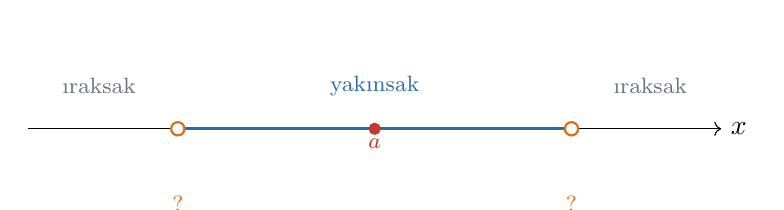
\begin{tikzpicture}[scale=1.0]
\draw[->] (-4.4,0)--(4.4,0) node[right]{$x$};
\draw[very thick,grafikMavi] (-2.5,0)--(2.5,0);
\filldraw[kirmizi] (0,0) circle (2pt) node[below]{\footnotesize $a$};
\filldraw[white,draw=turuncu,thick] (-2.5,0) circle (2.4pt) node[below=3pt]{\footnotesize $a-R$};
\filldraw[white,draw=turuncu,thick] (2.5,0) circle (2.4pt) node[below=3pt]{\footnotesize $a+R$};
\node[grafikMavi] at (0,0.55) {\footnotesize yakınsak};
\node[ortaGri] at (-3.5,0.55) {\footnotesize ıraksak};
\node[ortaGri] at (3.5,0.55) {\footnotesize ıraksak};
\node[turuncu] at (-2.5,-0.95) {\footnotesize ?};
\node[turuncu] at (2.5,-0.95) {\footnotesize ?};
\end{tikzpicture}
\end{center}

\soru{$\displaystyle\sum_{n=1}^{\infty}\frac{(x-2)^n}{n\,3^n}$ serisinin
yakınsaklık aralığını bulun.}

\cozum Oran testi:
$\left|\frac{a_{n+1}}{a_n}\right|=\frac{n}{n+1}\cdot\frac{|x-2|}{3}\to\frac{|x-2|}{3}<1$,
yani $|x-2|<3$: $R=3$ ve $-1<x<5$.
Uç noktalar: $x=5$'te $\sum\frac1n$ ıraksak; $x=-1$'de $\sum\frac{(-1)^n}{n}$
yakınsak. Sonuç: $[-1,5)$.

\pykontrol
\begin{lstlisting}
import sympy as sp
n, x = sp.symbols('n x')

c = 1/(n*3**n)
R = sp.limit(sp.Abs(c/c.subs(n, n + 1)), n, sp.oo)     # 3
print("R =", R, " aralik merkezi a = 2")

# Uc noktalari ayri incele
sp.summation(1/n, (n, 1, sp.oo))              # oo   -> x = 5 iraksak
sp.summation((-1)**n/n, (n, 1, sp.oo))        # -log(2) -> x = -1 yakinsak
\end{lstlisting}

\gsub{Bilinen Serilerden Yeni Seriler Türetme}

Geometrik seri, kuvvet serilerinin ana kaynağıdır:
\[
\frac{1}{1-x}=\sum_{n=0}^{\infty}x^n,\qquad |x|<1 .
\]
Bunu türeterek, integre ederek veya $x$ yerine başka ifade koyarak yeni seriler
elde ederiz.

\ornek{$x\to-x^2$ koyarsak $\dfrac{1}{1+x^2}=\sum(-1)^nx^{2n}$; integre edersek
\[
\arctan x=\sum_{n=0}^{\infty}\frac{(-1)^n x^{2n+1}}{2n+1},\qquad |x|\le1 .
\]
$x=1$ koyarsak $\dfrac{\pi}{4}=1-\frac13+\frac15-\frac17+\dots$ (Leibniz
formülü).}

\begin{lstlisting}
sp.series(1/(1 - x), x, 0, 6)            # 1 + x + x**2 + x**3 + x**4 + x**5 + O(x**6)
sp.series(sp.atan(x), x, 0, 8)           # x - x**3/3 + x**5/5 - x**7/7 + O(x**8)

# Leibniz formulunun yavas yakinsamasi
import numpy as np
k = np.arange(0, 100000)
print(4*np.sum((-1.0)**k/(2*k + 1)), np.pi)   # 3.14158... 3.14159...
\end{lstlisting}

% =====================================================================
\gsec{Taylor ve Maclaurin Serileri}
% =====================================================================

\kural[Taylor Serisi]{$f$ sonsuz türevlenebilirse $a$ merkezli açılımı:
\[
f(x)=\sum_{n=0}^{\infty}\frac{f^{(n)}(a)}{n!}(x-a)^n
=f(a)+f'(a)(x-a)+\frac{f''(a)}{2!}(x-a)^2+\dots
\]
$a=0$ hâline \emph{Maclaurin serisi} denir.}

\gsub{Ezberlenmesi Gereken Maclaurin Serileri}

\[
e^x=\sum_{n=0}^{\infty}\frac{x^n}{n!}=1+x+\frac{x^2}{2!}+\frac{x^3}{3!}+\dots
\qquad(\text{tüm } x)
\]
\[
\sin x=\sum_{n=0}^{\infty}\frac{(-1)^nx^{2n+1}}{(2n+1)!}
=x-\frac{x^3}{3!}+\frac{x^5}{5!}-\dots
\qquad(\text{tüm } x)
\]
\[
\cos x=\sum_{n=0}^{\infty}\frac{(-1)^nx^{2n}}{(2n)!}
=1-\frac{x^2}{2!}+\frac{x^4}{4!}-\dots
\qquad(\text{tüm } x)
\]
\[
\frac{1}{1-x}=\sum_{n=0}^{\infty}x^n=1+x+x^2+x^3+\dots
\qquad(|x|<1)
\]
\[
\ln(1+x)=\sum_{n=1}^{\infty}\frac{(-1)^{n-1}x^n}{n}
=x-\frac{x^2}{2}+\frac{x^3}{3}-\dots
\qquad(-1<x\le1)
\]
\[
\arctan x=\sum_{n=0}^{\infty}\frac{(-1)^nx^{2n+1}}{2n+1}
=x-\frac{x^3}{3}+\frac{x^5}{5}-\dots
\qquad(|x|\le1)
\]
\[
(1+x)^k=\sum_{n=0}^{\infty}\binom{k}{n}x^n
\qquad(|x|<1,\ \text{binom serisi})
\]
\[
\sinh x=\sum_{n=0}^{\infty}\frac{x^{2n+1}}{(2n+1)!},\qquad
\cosh x=\sum_{n=0}^{\infty}\frac{x^{2n}}{(2n)!}
\qquad(\text{tüm } x)
\]

\begin{lstlisting}
for f in [sp.exp(x), sp.sin(x), sp.cos(x), sp.log(1 + x), sp.atan(x)]:
    print(f, "=", sp.series(f, x, 0, 7))
\end{lstlisting}

\begin{lstlisting}[style=outstyle]
exp(x) = 1 + x + x**2/2 + x**3/6 + x**4/24 + x**5/120 + x**6/720 + O(x**7)
sin(x) = x - x**3/6 + x**5/120 + O(x**7)
cos(x) = 1 - x**2/2 + x**4/24 - x**6/720 + O(x**7)
log(x + 1) = x - x**2/2 + x**3/3 - x**4/4 + x**5/5 - x**6/6 + O(x**7)
atan(x) = x - x**3/3 + x**5/5 + O(x**7)
\end{lstlisting}

\bilgi{\code{sp.series(f, x, a, n)} sonucu $O(x^n)$ terimi içerir. Bu terimi
atmak için \code{.removeO()} kullan; polinom olarak çizim veya hesap yapmak
istediğinde gerekir.}

\gsub{Taylor Polinomu ve Yaklaşım}

$n$. mertebeden Taylor polinomu $T_n(x)$, serinin ilk $n+1$ terimidir. $n$
büyüdükçe yaklaşım iyileşir.

\begin{lstlisting}
import numpy as np, matplotlib.pyplot as plt, sympy as sp
x = sp.symbols('x')

f = sp.sin(x)
xs = np.linspace(-2*np.pi, 2*np.pi, 500)

plt.plot(xs, np.sin(xs), 'k', lw=2.5, label='sin(x)')
for N in [1, 3, 5, 7, 11]:
    T = sp.series(f, x, 0, N + 1).removeO()
    Tn = sp.lambdify(x, T, 'numpy')
    plt.plot(xs, Tn(xs) + 0*xs, lw=1.4, label=f'T{N}')

plt.ylim(-2, 2); plt.legend(); plt.grid(alpha=0.3)
plt.title('sin(x) ve Taylor polinomlari'); plt.show()
\end{lstlisting}

\ipucu{\code{Tn(xs) + 0*xs} yazmamızın nedeni: $T_1(x)=x$ gibi bir polinom
\code{lambdify} edildiğinde bazen skaler döndürür; \code{0*xs} eklemek sonucu
dizi hâline getirir.}

\gsub{Taylor Kalanı ve Hata Tahmini}

\teorem[Taylor Kalanı (Lagrange biçimi)]{
\[
f(x)=T_n(x)+R_n(x),\qquad
R_n(x)=\frac{f^{(n+1)}(c)}{(n+1)!}(x-a)^{n+1}
\]
olacak bir $c$, $a$ ile $x$ arasında vardır. Pratik sınır:
\[
|R_n(x)|\le\frac{M}{(n+1)!}|x-a|^{n+1},\qquad M=\max\bigl|f^{(n+1)}\bigr| .
\]}

\soru{$\sin(0.5)$ değerini $T_3$ ile hesaplayın ve hatayı sınırlayın.}

\cozum $T_3(x)=x-\frac{x^3}{6}$, $T_3(0.5)=0.5-0.0208333=0.4791667$.
Kalan: $|R_3|\le\frac{M}{4!}(0.5)^4$ ve $M=\max|f^{(4)}|=\max|\sin|\le1$;
$|R_3|\le\frac{0.0625}{24}\approx0.0026$. Gerçek değer $0.4794255$; gerçek
hata $0.00026$ --- sınırın içinde.

\pykontrol
\begin{lstlisting}
T3 = sp.series(sp.sin(x), x, 0, 4).removeO()      # x - x**3/6
yaklasim = float(T3.subs(x, 0.5))                  # 0.4791666666666667
gercek   = float(sp.sin(0.5))                      # 0.479425538604203
print(abs(gercek - yaklasim))                      # 0.000258871937536...

sinir = 1/sp.factorial(4)*sp.Rational(1,2)**4
float(sinir)                                        # 0.0026041666666666665
\end{lstlisting}

\begin{lstlisting}
def taylor_hata_grafigi(f, a=0, N_list=(1,3,5,7), aralik=(-3,3)):
    """Taylor polinomlarinin mutlak hatasini logaritmik olcekte cizer."""
    fn = sp.lambdify(x, f, 'numpy')
    xs = np.linspace(*aralik, 400)
    for N in N_list:
        T = sp.series(f, x, a, N + 1).removeO()
        Tn = sp.lambdify(x, T, 'numpy')
        plt.semilogy(xs, np.abs(fn(xs) - (Tn(xs) + 0*xs)) + 1e-18, label=f'T{N}')
    plt.legend(); plt.grid(alpha=0.3); plt.ylabel('mutlak hata'); plt.show()

taylor_hata_grafigi(sp.exp(x))
\end{lstlisting}

\gsub{Binom Serisi}

\kural{
\[
(1+x)^k=\sum_{n=0}^{\infty}\binom{k}{n}x^n,\qquad
\binom{k}{n}=\frac{k(k-1)\cdots(k-n+1)}{n!},\qquad |x|<1 .
\]
$k$ pozitif tam sayıysa seri sonlu (binom açılımı) olur.}

\ornek{$\sqrt{1+x}=(1+x)^{1/2}=1+\frac{x}{2}-\frac{x^2}{8}+\frac{x^3}{16}-\dots$
Bu, $\sqrt{1.1}\approx1.0488$ gibi hızlı tahminler için kullanılır.}

\begin{lstlisting}
sp.series(sp.sqrt(1 + x), x, 0, 5)
# 1 + x/2 - x**2/8 + x**3/16 - 5*x**4/128 + O(x**5)

k = sp.symbols('k')
sp.series((1 + x)**k, x, 0, 4)
\end{lstlisting}

\gsub{Serilerin Uygulamaları}

\gsubsub{1. Zor limitleri seriyle çözmek}

\soru{$\displaystyle\lm{x}{0}\frac{e^x-1-x}{x^2}$ limitini seri ile bulun.}

\cozum $e^x=1+x+\frac{x^2}{2}+\frac{x^3}{6}+\dots$ olduğundan pay
$\frac{x^2}{2}+\frac{x^3}{6}+\dots$; $x^2$'ye bölersek
$\frac12+\frac{x}{6}+\dots\to\frac12$.

\gsubsub{2. Temel olmayan integralleri hesaplamak}

\soru{$\displaystyle\int_0^1 e^{-x^2}dx$ integralini $10^{-4}$ hassasiyetle
seriyle hesaplayın.}

\cozum $e^{-x^2}=\sum\frac{(-1)^nx^{2n}}{n!}$; terim terim integre edelim:
\[
\int_0^1 e^{-x^2}dx=\sum_{n=0}^{\infty}\frac{(-1)^n}{n!(2n+1)}
=1-\frac13+\frac{1}{10}-\frac{1}{42}+\frac{1}{216}-\dots\approx0.7468 .
\]
Alterne seri olduğu için hata ilk atılan terimden küçüktür.

\begin{lstlisting}
S = sp.summation((-1)**n/(sp.factorial(n)*(2*n + 1)), (n, 0, 10))
float(S)                                        # 0.7468241328124271
float(sp.integrate(sp.exp(-x**2), (x, 0, 1)))   # 0.7468241328124271
\end{lstlisting}

\gsubsub{3. Diferansiyel denklemleri seriyle çözmek}

\begin{lstlisting}
y = sp.Function('y')
ode = sp.Eq(y(x).diff(x, 2) + x*y(x), 0)         # Airy denklemi
sp.dsolve(ode, y(x), hint='2nd_power_series_ordinary')
# y(x) = C0*(1 - x**3/6 + x**6/180 - ...) + C1*(x - x**4/12 + ...) + O(x**6)
\end{lstlisting}

\gsubsub{4. Euler formülü}

$e^{ix}=\cos x+i\sin x$ eşitliği, üç serinin yan yana konmasıyla görülür;
$x=\pi$ için $e^{i\pi}+1=0$ elde edilir.

\begin{lstlisting}
sp.expand(sp.exp(sp.I*x).rewrite(sp.cos))      # cos(x) + I*sin(x)
sp.simplify(sp.exp(sp.I*sp.pi) + 1)            # 0
\end{lstlisting}

% #####################################################################
\gpart{10}{Calculus 2 --- Parametrik Denklemler ve Kutupsal Koordinatlar}
% #####################################################################

% =====================================================================
\gsec{Parametrik Denklemler}
% =====================================================================

\tanim{Eğri, $x=x(t)$, $y=y(t)$ biçiminde bir $t$ parametresiyle verilirse
\emph{parametrik} olarak tanımlanmıştır. $t$ genelde zamandır; eğrinin
\emph{yönü} de belirlidir.}

\ornek{Çember: $x=r\cos t$, $y=r\sin t$, $t\in[0,2\pi]$.
Sikloid: $x=r(t-\sin t)$, $y=r(1-\cos t)$.
Elips: $x=a\cos t$, $y=b\sin t$.}

\begin{lstlisting}
import numpy as np, matplotlib.pyplot as plt

t = np.linspace(0, 4*np.pi, 800)
r = 1
plt.plot(r*(t - np.sin(t)), r*(1 - np.cos(t)), lw=2, color='#2E6DA4')
plt.axis('equal'); plt.grid(alpha=0.3); plt.title('Sikloid'); plt.show()
\end{lstlisting}

\gsub{Parametrik Türev}

\kural{
\[
\frac{dy}{dx}=\frac{dy/dt}{dx/dt}=\frac{y'(t)}{x'(t)},\qquad
\frac{d^2y}{dx^2}=\frac{\dfrac{d}{dt}\!\left(\dfrac{dy}{dx}\right)}{x'(t)} .
\]
Yatay teğet: $y'(t)=0$ (ve $x'(t)\neq0$); düşey teğet: $x'(t)=0$.}

\soru{$x=t^2$, $y=t^3-3t$ eğrisinin $t=2$ noktasındaki teğet eğimini bulun.}

\cozum $\frac{dy}{dx}=\frac{3t^2-3}{2t}$; $t=2$ için $\frac{12-3}{4}=\frac94$.

\pykontrol
\begin{lstlisting}
import sympy as sp
t = sp.symbols('t')

xt, yt = t**2, t**3 - 3*t
dydx = sp.simplify(sp.diff(yt, t)/sp.diff(xt, t))     # 3*(t**2 - 1)/(2*t)
dydx.subs(t, 2)                                        # 9/4

# Ikinci turev
d2ydx2 = sp.simplify(sp.diff(dydx, t)/sp.diff(xt, t))

# Yatay / dusey tegetler
sp.solve(sp.diff(yt, t), t)      # [-1, 1]  -> yatay teget
sp.solve(sp.diff(xt, t), t)      # [0]      -> dusey teget
\end{lstlisting}

\gsub{Parametrik Yay Uzunluğu ve Alan}

\kural{
\[
L=\int_{\alpha}^{\beta}\sqrt{\left(\frac{dx}{dt}\right)^2+\left(\frac{dy}{dt}\right)^2}\;dt,
\qquad
A=\int_{\alpha}^{\beta} y(t)\,x'(t)\dd t ,
\]
\[
S=2\pi\int_{\alpha}^{\beta} y(t)\sqrt{x'(t)^2+y'(t)^2}\;dt \quad(x\text{ ekseni etrafında}).
\]}

\soru{Bir kemer sikloidinin ($r=1$, $t\in[0,2\pi]$) uzunluğunu bulun.}

\cozum $x'=1-\cos t$, $y'=\sin t$;
$\sqrt{(1-\cos t)^2+\sin^2t}=\sqrt{2-2\cos t}=2\left|\sin\frac t2\right|$.
\[
L=\int_0^{2\pi}2\sin\frac t2\,dt=\Bigl[-4\cos\tfrac t2\Bigr]_0^{2\pi}=8 .
\]

\begin{lstlisting}
xt, yt = t - sp.sin(t), 1 - sp.cos(t)
ds = sp.sqrt(sp.diff(xt, t)**2 + sp.diff(yt, t)**2)
L = sp.integrate(sp.simplify(ds), (t, 0, 2*sp.pi))     # 8

A = sp.integrate(yt*sp.diff(xt, t), (t, 0, 2*sp.pi))   # 3*pi
\end{lstlisting}

% =====================================================================
\gsec{Kutupsal Koordinatlar (Polar Coordinates)}
% =====================================================================

\kural{Dönüşümler:
\[
x=r\cos\theta,\quad y=r\sin\theta,\qquad
r^2=x^2+y^2,\quad \tan\theta=\frac{y}{x} .
\]}

\begin{center}
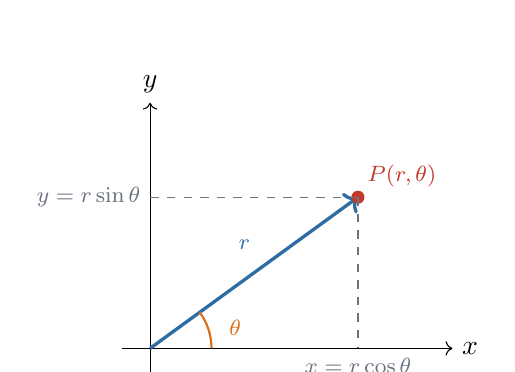
\begin{tikzpicture}[scale=1.2]
\draw[->] (-0.3,0)--(3.2,0) node[right]{$x$};
\draw[->] (0,-0.3)--(0,2.6) node[above]{$y$};
\draw[grafikMavi,very thick,->] (0,0)--(2.2,1.6);
\filldraw[kirmizi] (2.2,1.6) circle (1.8pt) node[above right]{\footnotesize $P(r,\theta)$};
\draw[dashed,ortaGri] (2.2,1.6)--(2.2,0) node[below]{\footnotesize $x=r\cos\theta$};
\draw[dashed,ortaGri] (2.2,1.6)--(0,1.6) node[left]{\footnotesize $y=r\sin\theta$};
\draw[turuncu,thick] (0.65,0)  arc (0:36:0.65);
\node[turuncu] at (0.9,0.22) {\footnotesize $\theta$};
\node[grafikMavi] at (1.0,1.1) {\footnotesize $r$};
\end{tikzpicture}
\end{center}

\gsub{Önemli Kutupsal Eğriler}

\begin{center}
\begin{tabularx}{\textwidth}{@{}>{$\displaystyle}l<{$} X@{}}
\toprule
\rowcolor{acikMavi}\multicolumn{1}{@{}l}{\color{anaMavi}\textbf{Denklem}} & \multicolumn{1}{l@{}}{\color{anaMavi}\textbf{Eğri}}\\
\midrule
r=a & Merkezi orijinde $a$ yarıçaplı çember.\\
\rowcolor{acikGri} r=2a\cos\theta & Merkezi $(a,0)$ olan çember.\\
r=a(1+\cos\theta) & Kardioid (kalp eğrisi).\\
\rowcolor{acikGri} r=a\cos(n\theta) & Gül eğrisi: $n$ tek ise $n$, çift ise $2n$ yaprak.\\
r^2=a^2\cos2\theta & Lemniskat (sonsuz işareti).\\
\rowcolor{acikGri} r=a\theta & Arşimet spirali.\\
\bottomrule
\end{tabularx}
\end{center}

\begin{lstlisting}
import numpy as np, matplotlib.pyplot as plt

th = np.linspace(0, 2*np.pi, 1000)
egriler = {'Kardioid': 1 + np.cos(th),
           'Gul (n=3)': np.cos(3*th),
           'Spiral': 0.2*th}

fig, axes = plt.subplots(1, 3, figsize=(12, 4),
                         subplot_kw={'projection': 'polar'})
for ax, (ad, r) in zip(axes, egriler.items()):
    ax.plot(th, r, lw=2, color='#2E6DA4')
    ax.set_title(ad)
plt.tight_layout(); plt.show()
\end{lstlisting}

\gsub{Kutupsal Türev}

\kural{$r=f(\theta)$ eğrisi için
\[
\frac{dy}{dx}=\frac{\dfrac{dr}{d\theta}\sin\theta+r\cos\theta}
                   {\dfrac{dr}{d\theta}\cos\theta-r\sin\theta} .
\]}

\begin{lstlisting}
th = sp.symbols('theta')
r = 1 + sp.cos(th)                      # kardioid

xs_, ys_ = r*sp.cos(th), r*sp.sin(th)
dydx = sp.simplify(sp.diff(ys_, th)/sp.diff(xs_, th))
dydx.subs(th, sp.pi/2)                  # tegetin egimi
\end{lstlisting}

\gsub{Kutupsal Alan ve Yay Uzunluğu}

\kural{
\[
A=\frac12\int_{\alpha}^{\beta}\bigl[f(\theta)\bigr]^2 d\theta,
\qquad
L=\int_{\alpha}^{\beta}\sqrt{r^2+\left(\frac{dr}{d\theta}\right)^2}\;d\theta .
\]
İki eğri arasındaki alan: $A=\frac12\int(r_{\text{dış}}^2-r_{\text{iç}}^2)d\theta$.}

\soru{$r=1+\cos\theta$ kardioidinin çevrelediği alanı bulun.}

\cozum
\[
A=\frac12\int_0^{2\pi}(1+\cos\theta)^2d\theta
=\frac12\int_0^{2\pi}\left(1+2\cos\theta+\frac{1+\cos2\theta}{2}\right)d\theta
=\frac{3\pi}{2}.
\]

\pykontrol
\begin{lstlisting}
r = 1 + sp.cos(th)
A = sp.integrate(r**2/2, (th, 0, 2*sp.pi))            # 3*pi/2

dr = sp.diff(r, th)
L = sp.integrate(sp.sqrt(r**2 + dr**2), (th, 0, 2*sp.pi))   # 8
\end{lstlisting}

\soru{$r=\cos 2\theta$ gül eğrisinin \emph{bir} yaprağının alanını bulun.}

\cozum Yaprak $\theta\in[-\pi/4,\pi/4]$ aralığında çizilir:
\[
A=\frac12\int_{-\pi/4}^{\pi/4}\cos^2 2\theta\,d\theta=\frac{\pi}{8}.
\]

\begin{lstlisting}
sp.integrate(sp.cos(2*th)**2/2, (th, -sp.pi/4, sp.pi/4))    # pi/8
\end{lstlisting}

\gsub{Kutupsal Eğrilerde Simetri ve Kesişim}

\ipucu{Simetri testleri çizimi çok hızlandırır:
\begin{itemize}\itemsep1pt
\item $\theta\to-\theta$ denklemi değiştirmiyorsa eğri \emph{kutup eksenine}
($x$ ekseni) göre simetriktir --- $r=1+\cos\theta$ gibi.
\item $\theta\to\pi-\theta$ değiştirmiyorsa $\theta=\pi/2$ doğrusuna
($y$ ekseni) göre simetriktir --- $r=1+\sin\theta$ gibi.
\item $r\to-r$ (veya $\theta\to\theta+\pi$) değiştirmiyorsa orijine göre
simetriktir.
\end{itemize}}

\uyari{Kutupsal eğrilerin kesişimini bulurken $r_1(\theta)=r_2(\theta)$
denklemini çözmek \textbf{yetmez}: aynı nokta farklı $(r,\theta)$ çiftleriyle
yazılabilir ve \emph{kutup} (orijin) çoğu zaman denklemde görünmeyen bir
kesişimdir. Her zaman iki eğriyi birlikte çizip kontrol et.}

\ornek{$r=1+\cos\theta$ (kardioid) ile $r=3\cos\theta$ (çember):
$1+\cos\theta=3\cos\theta \Rightarrow \cos\theta=\tfrac12
\Rightarrow \theta=\pm\pi/3$. Ancak grafikten görülür ki iki eğri
\emph{orijinde} de kesişir --- kardioid $\theta=\pi$'de, çember
$\theta=\pi/2$'de oraya ulaşır. Denklem bu kesişimi vermez.}

\begin{lstlisting}
import numpy as np, matplotlib.pyplot as plt

th = np.linspace(0, 2*np.pi, 1000)
ax = plt.subplot(projection='polar')
ax.plot(th, 1 + np.cos(th), lw=2, label='kardioid')
ax.plot(th, 3*np.cos(th), lw=2, label='cember')
ax.legend(loc='upper right'); plt.show()
\end{lstlisting}

% =====================================================================
\gsec{Konikler (Conic Sections)}
% =====================================================================

Bir koniyi bir düzlemle kesince ortaya çıkan üç eğri --- parabol, elips ve
hiperbol --- gezegen yörüngelerinden anten tasarımına kadar her yerdedir.

\gsub{Parabol}

\tanim{Sabit bir noktaya (\emph{odak}) ve sabit bir doğruya
(\emph{doğrultman/directrix}) eşit uzaklıktaki noktaların kümesi.
Tepe noktası orijinde ve ekseni $x$ ekseni olan parabol:
\[
y^2=4px,\qquad \text{odak } (p,0),\qquad \text{doğrultman } x=-p .
\]}

\ornek{Parabolik antenin çalışma ilkesi: eksene paralel gelen tüm ışınlar
yansıdıktan sonra \emph{tek bir noktada} --- odakta --- toplanır. Bu, teğet
doğrusunun türevle bulunan eğiminden ispatlanır.}

\gsub{Elips}

\tanim{İki sabit noktaya (odaklar) uzaklıkları toplamı sabit olan noktalar:
\[
\frac{x^2}{a^2}+\frac{y^2}{b^2}=1,\qquad
c^2=a^2-b^2,\qquad
\text{odaklar }(\pm c,0),\qquad
e=\frac{c}{a}<1 .
\]
Alanı $\pi ab$'dir; çevresi ise temel fonksiyonlarla ifade edilemez (eliptik
integral gerektirir).}

\begin{lstlisting}
import sympy as sp
x, a, b = sp.symbols('x a b', positive=True)

# Elips alani: 2 * integral( b*sqrt(1 - x^2/a^2) ) dx, -a..a
A = 2*sp.integrate(b*sp.sqrt(1 - x**2/a**2), (x, -a, a))
sp.simplify(A)                      # pi*a*b
\end{lstlisting}

\gsub{Hiperbol}

\tanim{İki odağa uzaklıkları \emph{farkı} sabit olan noktalar:
\[
\frac{x^2}{a^2}-\frac{y^2}{b^2}=1,\qquad
c^2=a^2+b^2,\qquad
\text{asimptotlar } y=\pm\frac{b}{a}x,\qquad e=\frac{c}{a}>1 .
\]}

\begin{center}
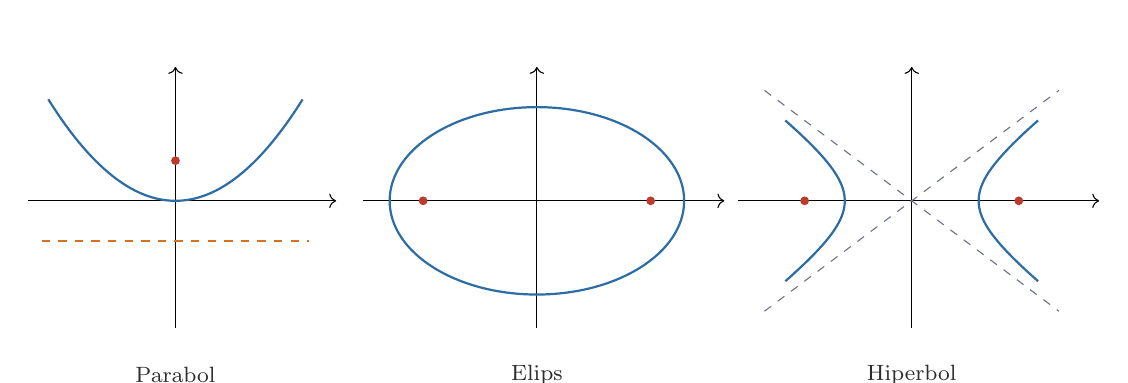
\begin{tikzpicture}[scale=0.85]
\begin{scope}
\draw[->] (-2.2,0)--(2.4,0); \draw[->] (0,-1.9)--(0,2.0);
\draw[grafikMavi,thick,domain=-1.9:1.9,samples=60] plot (\x,{0.42*\x*\x});
\filldraw[kirmizi] (0,0.6) circle (1.6pt);
\draw[dashed,turuncu] (-2.0,-0.6)--(2.0,-0.6);
\node[koyuGri] at (0,-2.6) {\footnotesize Parabol};
\end{scope}
\begin{scope}[xshift=5.4cm]
\draw[->] (-2.6,0)--(2.8,0); \draw[->] (0,-1.9)--(0,2.0);
\draw[grafikMavi,thick] (0,0) ellipse (2.2 and 1.4);
\filldraw[kirmizi] (1.7,0) circle (1.6pt);
\filldraw[kirmizi] (-1.7,0) circle (1.6pt);
\node[koyuGri] at (0,-2.6) {\footnotesize Elips};
\end{scope}
\begin{scope}[xshift=11cm]
\draw[->] (-2.6,0)--(2.8,0); \draw[->] (0,-1.9)--(0,2.0);
\draw[dashed,ortaGri] (-2.2,-1.65)--(2.2,1.65);
\draw[dashed,ortaGri] (-2.2,1.65)--(2.2,-1.65);
\draw[grafikMavi,thick,domain=0:1.25,samples=60] plot ({1*(exp(\x)+exp(-\x))/2},{0.75*(exp(\x)-exp(-\x))/2});
\draw[grafikMavi,thick,domain=0:1.25,samples=60] plot ({1*(exp(\x)+exp(-\x))/2},{-0.75*(exp(\x)-exp(-\x))/2});
\draw[grafikMavi,thick,domain=0:1.25,samples=60] plot ({-1*(exp(\x)+exp(-\x))/2},{0.75*(exp(\x)-exp(-\x))/2});
\draw[grafikMavi,thick,domain=0:1.25,samples=60] plot ({-1*(exp(\x)+exp(-\x))/2},{-0.75*(exp(\x)-exp(-\x))/2});
\filldraw[kirmizi] (1.6,0) circle (1.6pt);
\filldraw[kirmizi] (-1.6,0) circle (1.6pt);
\node[koyuGri] at (0,-2.6) {\footnotesize Hiperbol};
\end{scope}
\end{tikzpicture}
\end{center}
\vspace{1.1cm}

\begin{center}
\renewcommand{\arraystretch}{2.4}
\begin{tabularx}{\textwidth}{@{}>{\bfseries\color{anaMavi}}l >{$\displaystyle}l<{$} X@{}}
\toprule
\rowcolor{acikMavi}\multicolumn{1}{@{}l}{\color{anaMavi}\textbf{Konik}} & \multicolumn{1}{l}{\color{anaMavi}\textbf{Standart biçim}} & \multicolumn{1}{l@{}}{\color{anaMavi}\textbf{Dış merkezlik}}\\
\midrule
Parabol & y^2=4px & $e=1$; odak $(p,0)$\\
\rowcolor{acikGri} Elips & \frac{x^2}{a^2}+\frac{y^2}{b^2}=1 & $e=c/a<1$; $c^2=a^2-b^2$\\
Hiperbol & \frac{x^2}{a^2}-\frac{y^2}{b^2}=1 & $e=c/a>1$; $c^2=a^2+b^2$\\
\bottomrule
\end{tabularx}
\end{center}

\gsub{Koniklerin Kutupsal Biçimi}

\kural{Odak orijinde olmak üzere üç konik \emph{tek} bir denklemle yazılır:
\[
r=\frac{ed}{1+e\cos\theta}
\]
Burada $e$ dış merkezlik, $d$ odak--doğrultman uzaklığıdır.
$e<1$ elips, $e=1$ parabol, $e>1$ hiperbol verir. Doğrultman yatay ise
$\cos\theta$ yerine $\sin\theta$ yazılır.}

\ornek[Gezegen Yörüngeleri]{Kepler'in birinci yasası: gezegenler, Güneş
odaklardan birinde olacak şekilde elips çizer. Dünya için $e\approx0{,}017$
(neredeyse çember), Halley kuyruklu yıldızı için $e\approx0{,}967$ (çok basık
elips). Bu yüzden yörünge hesapları doğrudan yukarıdaki kutupsal formülle
yapılır.}

\begin{lstlisting}
import numpy as np, matplotlib.pyplot as plt

th = np.linspace(0, 2*np.pi, 1000)
for e, ad in [(0.5, 'elips'), (1.0, 'parabol'), (1.6, 'hiperbol')]:
    r = (1*e)/(1 + e*np.cos(th))
    r = np.where(r > 0, r, np.nan)          # negatif kollari gizle
    plt.polar(th, r, lw=2, label=f'{ad} (e={e})')
plt.legend(loc='upper right'); plt.show()
\end{lstlisting}

\begin{lstlisting}
# Konigi denklemden tanima: diskriminant testi
# A x^2 + B xy + C y^2 + ... = 0  icin  B^2 - 4AC
# < 0 elips, = 0 parabol, > 0 hiperbol
import sympy as sp
x, y = sp.symbols('x y')
for A, B, C in [(1, 0, 4), (1, 0, 0), (1, 0, -1)]:
    d = B**2 - 4*A*C
    tur = 'elips' if d < 0 else ('parabol' if d == 0 else 'hiperbol')
    print(f"B^2-4AC = {d:>3}  ->  {tur}")
\end{lstlisting}

% #####################################################################
\gpart{11}{Referans: Formüller ve Python Sözlüğü}
% #####################################################################

% =====================================================================
\gsec{Limit Formülleri}
% =====================================================================

\gsub{Özel Limitler}

\begin{center}
\renewcommand{\arraystretch}{3.0}
\begin{tabularx}{\textwidth}{@{}>{$\displaystyle}X<{$} >{$\displaystyle}X<{$}@{}}
\toprule
\rowcolor{acikMavi}\multicolumn{1}{@{}l}{\color{anaMavi}\textbf{Limit}} & \multicolumn{1}{l@{}}{\color{anaMavi}\textbf{Limit}}\\
\midrule
\lm{x}{0}\frac{\sin x}{x}=1 & \lm{x}{0}\frac{\tan x}{x}=1\\
\rowcolor{acikGri} \lm{x}{0}\frac{1-\cos x}{x}=0 & \lm{x}{0}\frac{1-\cos x}{x^2}=\frac12\\
\lm{x}{0}\frac{e^x-1}{x}=1 & \lm{x}{0}\frac{\ln(1+x)}{x}=1\\
\rowcolor{acikGri} \lm{x}{0}\frac{a^x-1}{x}=\ln a & \lm{x}{0}\frac{(1+x)^k-1}{x}=k\\
\lim_{x\to\infty}\left(1+\frac{1}{x}\right)^x=e & \lim_{x\to\infty}\left(1+\frac{k}{x}\right)^x=e^k\\
\rowcolor{acikGri} \lim_{x\to\infty}\frac{\ln x}{x^p}=0\ (p>0) & \lim_{x\to\infty}\frac{x^p}{e^x}=0\\
\lim_{n\to\infty}\sqrt[n]{n}=1 & \lim_{n\to\infty}\frac{n!}{n^n}=0\\
\bottomrule
\end{tabularx}
\end{center}

% =====================================================================
\gsec{Türev Formülleri (Tam Liste)}
% =====================================================================

\begin{center}
\renewcommand{\arraystretch}{2.4}
\begin{tabularx}{\textwidth}{@{}>{$\displaystyle}X<{$} >{$\displaystyle}X<{$}@{}}
\toprule
\rowcolor{acikMavi}\multicolumn{1}{@{}l}{\color{anaMavi}\textbf{Kural / Fonksiyon}} & \multicolumn{1}{l@{}}{\color{anaMavi}\textbf{Türev}}\\
\midrule
\bigl(x^n\bigr)' & n x^{n-1}\\
\rowcolor{acikGri} (fg)' & f'g+fg'\\
\left(\frac{f}{g}\right)' & \frac{f'g-fg'}{g^2}\\
\rowcolor{acikGri} \bigl(f(g(x))\bigr)' & f'(g(x))g'(x)\\
\bigl(f^{-1}\bigr)'(x) & \frac{1}{f'\bigl(f^{-1}(x)\bigr)}\\
\rowcolor{acikGri} \bigl(\sin x\bigr)',\ \bigl(\cos x\bigr)' & \cos x,\quad -\sin x\\
\bigl(\tan x\bigr)',\ \bigl(\cot x\bigr)' & \sec^2x,\quad -\csc^2x\\
\rowcolor{acikGri} \bigl(\sec x\bigr)',\ \bigl(\csc x\bigr)' & \sec x\tan x,\quad -\csc x\cot x\\
\bigl(e^x\bigr)',\ \bigl(a^x\bigr)' & e^x,\quad a^x\ln a\\
\rowcolor{acikGri} \bigl(\ln x\bigr)',\ \bigl(\log_a x\bigr)' & \frac1x,\quad \frac{1}{x\ln a}\\
\bigl(\arcsin x\bigr)',\ \bigl(\arccos x\bigr)' & \frac{1}{\sqrt{1-x^2}},\quad -\frac{1}{\sqrt{1-x^2}}\\
\rowcolor{acikGri} \bigl(\arctan x\bigr)',\ \bigl(\operatorname{arccot} x\bigr)' & \frac{1}{1+x^2},\quad -\frac{1}{1+x^2}\\
\bigl(\sinh x\bigr)',\ \bigl(\cosh x\bigr)' & \cosh x,\quad \sinh x\\
\rowcolor{acikGri} \bigl(\tanh x\bigr)' & \operatorname{sech}^2x\\
\bigl(u^v\bigr)' & u^v\left(v'\ln u+\frac{vu'}{u}\right)\\
\bottomrule
\end{tabularx}
\end{center}

% =====================================================================
\gsec{İntegral Formülleri (Tam Liste)}
% =====================================================================

\gsub{Temel ve Trigonometrik}

\begin{center}
\renewcommand{\arraystretch}{3.0}
\begin{tabularx}{\textwidth}{@{}>{$\displaystyle}X<{$} >{$\displaystyle}X<{$}@{}}
\toprule
\rowcolor{acikMavi}\multicolumn{1}{@{}l}{\color{anaMavi}\textbf{İntegral}} & \multicolumn{1}{l@{}}{\color{anaMavi}\textbf{Sonuç ($+C$)}}\\
\midrule
\int x^n dx\ (n\neq-1) & \frac{x^{n+1}}{n+1}\\
\rowcolor{acikGri} \int \frac{dx}{x} & \ln|x|\\
\int e^{ax}dx & \frac{e^{ax}}{a}\\
\rowcolor{acikGri} \int a^x dx & \frac{a^x}{\ln a}\\
\int \ln x\,dx & x\ln x-x\\
\rowcolor{acikGri} \int \sin x\,dx,\ \int\cos x\,dx & -\cos x,\quad \sin x\\
\int \tan x\,dx & -\ln|\cos x|=\ln|\sec x|\\
\rowcolor{acikGri} \int \cot x\,dx & \ln|\sin x|\\
\int \sec x\,dx & \ln|\sec x+\tan x|\\
\rowcolor{acikGri} \int \csc x\,dx & -\ln|\csc x+\cot x|\\
\int \sec^2x\,dx,\ \int\csc^2x\,dx & \tan x,\quad -\cot x\\
\rowcolor{acikGri} \int \sec x\tan x\,dx & \sec x\\
\int \sin^2x\,dx & \frac{x}{2}-\frac{\sin 2x}{4}\\
\rowcolor{acikGri} \int \cos^2x\,dx & \frac{x}{2}+\frac{\sin 2x}{4}\\
\bottomrule
\end{tabularx}
\end{center}

\gsub{Ters Trigonometrik ve Hiperbolik Sonuçlar}

\begin{center}
\renewcommand{\arraystretch}{3.0}
\begin{tabularx}{\textwidth}{@{}>{$\displaystyle}X<{$} >{$\displaystyle}X<{$}@{}}
\toprule
\rowcolor{acikMavi}\multicolumn{1}{@{}l}{\color{anaMavi}\textbf{İntegral}} & \multicolumn{1}{l@{}}{\color{anaMavi}\textbf{Sonuç ($+C$)}}\\
\midrule
\int\frac{dx}{a^2+x^2} & \frac1a\arctan\frac{x}{a}\\
\rowcolor{acikGri} \int\frac{dx}{\sqrt{a^2-x^2}} & \arcsin\frac{x}{a}\\
\int\frac{dx}{x\sqrt{x^2-a^2}} & \frac1a\operatorname{arcsec}\left|\frac{x}{a}\right|\\
\rowcolor{acikGri} \int\frac{dx}{\sqrt{x^2+a^2}} & \ln\left|x+\sqrt{x^2+a^2}\right|=\operatorname{arsinh}\frac{x}{a}\\
\int\frac{dx}{\sqrt{x^2-a^2}} & \ln\left|x+\sqrt{x^2-a^2}\right|\\
\rowcolor{acikGri} \int\frac{dx}{a^2-x^2} & \frac{1}{2a}\ln\left|\frac{a+x}{a-x}\right|\\
\int\sqrt{a^2-x^2}\,dx & \frac{x\sqrt{a^2-x^2}}{2}+\frac{a^2}{2}\arcsin\frac{x}{a}\\
\rowcolor{acikGri} \int\sinh x\,dx,\ \int\cosh x\,dx & \cosh x,\quad \sinh x\\
\bottomrule
\end{tabularx}
\end{center}

\gsub{Uygulama Formülleri}

\begin{center}
\renewcommand{\arraystretch}{3.0}
\begin{tabularx}{\textwidth}{@{}>{\bfseries\color{anaMavi}}l >{$\displaystyle}X<{$}@{}}
\toprule
\rowcolor{acikMavi}\multicolumn{1}{@{}l}{\color{anaMavi}\textbf{Büyüklük}} & \multicolumn{1}{l@{}}{\color{anaMavi}\textbf{Formül}}\\
\midrule
Alan (iki eğri) & A=\int_a^b\bigl(f-g\bigr)dx\\
\rowcolor{acikGri} Hacim (disk/halka) & V=\pi\int_a^b\bigl(R^2-r^2\bigr)dx\\
Hacim (kabuk) & V=2\pi\int_a^b x f(x)\,dx\\
\rowcolor{acikGri} Kesitli hacim & V=\int_a^b A(x)\,dx\\
Yay uzunluğu & L=\int_a^b\sqrt{1+(f')^2}\,dx\\
\rowcolor{acikGri} Yüzey alanı & S=2\pi\int_a^b f\sqrt{1+(f')^2}\,dx\\
Ortalama değer & f_{\text{ort}}=\frac{1}{b-a}\int_a^b f\,dx\\
\rowcolor{acikGri} İş & W=\int_a^b F(x)\,dx\\
Parametrik uzunluk & L=\int_{\alpha}^{\beta}\sqrt{x'(t)^2+y'(t)^2}\,dt\\
\rowcolor{acikGri} Kutupsal alan & A=\frac12\int_{\alpha}^{\beta}r^2\,d\theta\\
Kutupsal uzunluk & L=\int_{\alpha}^{\beta}\sqrt{r^2+(r')^2}\,d\theta\\
\bottomrule
\end{tabularx}
\end{center}

% =====================================================================
\gsec{Seri Formülleri}
% =====================================================================

\begin{center}
\renewcommand{\arraystretch}{3.0}
\begin{tabularx}{\textwidth}{@{}>{$\displaystyle}X<{$} X@{}}
\toprule
\rowcolor{acikMavi}\multicolumn{1}{@{}l}{\color{anaMavi}\textbf{Seri}} & \multicolumn{1}{l@{}}{\color{anaMavi}\textbf{Not}}\\
\midrule
\sum_{n=0}^{\infty}ar^n=\frac{a}{1-r} & $|r|<1$ (geometrik)\\
\rowcolor{acikGri} \sum_{n=1}^{\infty}\frac{1}{n^p} & $p>1$ yakınsak, $p\le1$ ıraksak\\
\sum_{n=1}^{\infty}\frac{1}{n^2}=\frac{\pi^2}{6} & Basel problemi\\
\rowcolor{acikGri} \sum_{n=1}^{\infty}\frac{(-1)^{n-1}}{n}=\ln 2 & Alterne harmonik\\
\sum_{n=0}^{\infty}\frac{(-1)^n}{2n+1}=\frac{\pi}{4} & Leibniz formülü\\
\rowcolor{acikGri} \sum_{n=0}^{\infty}\frac{1}{n!}=e & Üstel seri, $x=1$\\
\sum_{k=1}^{n}k=\frac{n(n+1)}{2} & Sonlu toplam\\
\rowcolor{acikGri} \sum_{k=1}^{n}k^2=\frac{n(n+1)(2n+1)}{6} & Riemann toplamlarında\\
\sum_{k=1}^{n}k^3=\left(\frac{n(n+1)}{2}\right)^2 & Sonlu toplam\\
\bottomrule
\end{tabularx}
\end{center}

% =====================================================================
\gsec{Trigonometrik Özdeşlikler}
% =====================================================================

\[
\sin^2x+\cos^2x=1,\qquad 1+\tan^2x=\sec^2x,\qquad 1+\cot^2x=\csc^2x
\]
\[
\sin 2x=2\sin x\cos x,\qquad \cos2x=\cos^2x-\sin^2x=1-2\sin^2x=2\cos^2x-1
\]
\[
\sin^2x=\frac{1-\cos2x}{2},\qquad \cos^2x=\frac{1+\cos2x}{2}
\]
\[
\sin(A\pm B)=\sin A\cos B\pm\cos A\sin B,\qquad
\cos(A\pm B)=\cos A\cos B\mp\sin A\sin B
\]
\[
\cosh^2x-\sinh^2x=1,\qquad \sinh x=\frac{e^x-e^{-x}}{2},\qquad
\cosh x=\frac{e^x+e^{-x}}{2}
\]

% =====================================================================
\gsec{Python Sözlüğü: Hangi İş İçin Hangi Komut?}
% =====================================================================

\gsub{SymPy --- Sembolik}

\begin{center}
\begin{tabularx}{\textwidth}{@{}>{\ttfamily\color{anaMavi}}l X@{}}
\toprule
\rowcolor{acikMavi}\multicolumn{1}{@{}l}{\color{anaMavi}\textbf{Komut}} & \multicolumn{1}{l@{}}{\color{anaMavi}\textbf{İş}}\\
\midrule
symbols('x y') & Sembol tanımlar.\\
\rowcolor{acikGri} limit(f, x, a, dir) & Limit; \code{dir='+'}, \code{'-'} veya \code{'+-'}.\\
diff(f, x, n) & $n$. mertebeden türev.\\
\rowcolor{acikGri} idiff(eq, y, x) & Kapalı türev.\\
integrate(f, x) & Belirsiz integral.\\
\rowcolor{acikGri} integrate(f, (x,a,b)) & Belirli / genelleştirilmiş integral.\\
series(f, x, a, n) & Taylor açılımı; \code{.removeO()} ile $O$ terimini at.\\
\rowcolor{acikGri} summation(a, (n,1,oo)) & Seri toplamı.\\
solve / solveset & Denklem çözer.\\
\rowcolor{acikGri} nsolve(f, x, x0) & Sayısal kök.\\
dsolve(ode, y(x), ics=...) & Diferansiyel denklem çözer.\\
\rowcolor{acikGri} classify\_ode(ode) & Denklemin tipini söyler.\\
apart / together & Kısmi kesir / ortak payda.\\
\rowcolor{acikGri} simplify / trigsimp & Sadeleştirme.\\
lambdify(x, f, 'numpy') & Sembolik ifadeyi hızlı sayısal fonksiyona çevirir.\\
\rowcolor{acikGri} evalf(k) & $k$ basamak ondalık değer.\\
Rational(a,b) & Tam kesir (float kaybını önler).\\
\rowcolor{acikGri} oo, pi, E, I & $\infty$, $\pi$, $e$, $i$.\\
\bottomrule
\end{tabularx}
\end{center}

\gsub{NumPy / SciPy / Matplotlib --- Sayısal}

\begin{center}
\begin{tabularx}{\textwidth}{@{}>{\ttfamily\color{anaMavi}}l X@{}}
\toprule
\rowcolor{acikMavi}\multicolumn{1}{@{}l}{\color{anaMavi}\textbf{Komut}} & \multicolumn{1}{l@{}}{\color{anaMavi}\textbf{İş}}\\
\midrule
np.linspace(a,b,n) & Eşit aralıklı örnekleme (grafik ve Riemann için).\\
\rowcolor{acikGri} np.gradient(y,x) & Veriden sayısal türev.\\
np.trapz(y,x) & Yamuk kuralıyla integral.\\
\rowcolor{acikGri} np.cumsum(v) & Kısmi toplam dizisi (seriler için).\\
scipy.integrate.quad & Adaptif sayısal integral (\code{np.inf} sınırlar olur).\\
\rowcolor{acikGri} scipy.integrate.simpson & Örneklenmiş veriden Simpson integrali.\\
scipy.integrate.solve\_ivp & Diferansiyel denklem sayısal çözümü.\\
\rowcolor{acikGri} scipy.optimize.brentq & Aralıkta güvenli kök bulma.\\
scipy.optimize.minimize\_scalar & Tek değişkenli optimizasyon.\\
\rowcolor{acikGri} scipy.misc.derivative & (eski) sayısal türev; merkezî farkı kendin yaz.\\
plt.fill\_between & Eğri altındaki alanı boyar.\\
\rowcolor{acikGri} plt.quiver & Yön alanı çizer.\\
plt.polar & Kutupsal grafik.\\
\bottomrule
\end{tabularx}
\end{center}

\gsub{Hızlı Tarif Kitabı}

\begin{lstlisting}
import sympy as sp, numpy as np, matplotlib.pyplot as plt
x, t, n = sp.symbols('x t n')

# 1) Limit (iki tarafli)
sp.limit(sp.sin(x)/x, x, 0, '+-')

# 2) Turev + teget dogrusu
f = x**3 - 2*x; a = 1
teget = f.subs(x, a) + sp.diff(f, x).subs(x, a)*(x - a)

# 3) Kritik noktalar ve tur tayini
kritik = sp.solve(sp.diff(f, x), x)
[(c, sp.diff(f, x, 2).subs(x, c)) for c in kritik]

# 4) Belirli integral (sembolik + sayisal)
sp.integrate(sp.exp(-x**2), (x, 0, 1))
from scipy.integrate import quad
quad(lambda u: np.exp(-u**2), 0, 1)[0]

# 5) Egri alti alani cizmek
xs = np.linspace(0, 1, 300)
plt.plot(xs, np.exp(-xs**2)); plt.fill_between(xs, np.exp(-xs**2), alpha=0.3)

# 6) Seri toplami ve yakinsaklik
sp.summation(1/n**2, (n, 1, sp.oo))

# 7) Taylor polinomu
sp.series(sp.exp(x), x, 0, 6).removeO()

# 8) Diferansiyel denklem
y = sp.Function('y')
sp.dsolve(sp.Eq(y(x).diff(x) + 2*y(x), sp.exp(-x)), y(x))

# 9) Donel hacim (disk)
sp.pi*sp.integrate(sp.sqrt(x)**2, (x, 0, 4))

# 10) Yay uzunlugu
sp.integrate(sp.sqrt(1 + sp.diff(sp.sqrt(x), x)**2), (x, 1, 4))
\end{lstlisting}

% =====================================================================
\gsec{Genel Bakış: Kavramlar Nasıl Bağlanıyor?}
% =====================================================================

\begin{center}
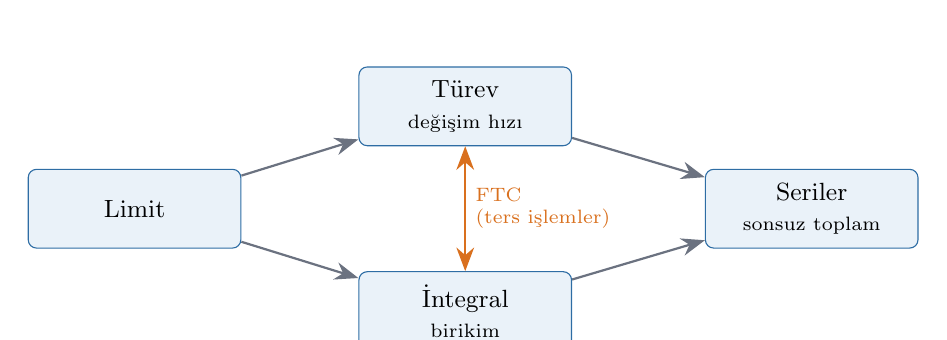
\begin{tikzpicture}[scale=1.0,
  kutu/.style={draw=vurguMavi,fill=acikMavi,rounded corners=3pt,
               minimum width=2.7cm,minimum height=1cm,align=center,font=\small},
  ok/.style={-{Stealth[length=3mm]},thick,ortaGri}]
\node[kutu] (lim) at (0,0) {Limit};
\node[kutu] (tur) at (4.2,1.3) {Türev\\ \scriptsize değişim hızı};
\node[kutu] (int) at (4.2,-1.3) {İntegral\\ \scriptsize birikim};
\node[kutu] (ser) at (8.6,0) {Seriler\\ \scriptsize sonsuz toplam};
\draw[ok] (lim) -- (tur);
\draw[ok] (lim) -- (int);
\draw[ok] (tur) -- (ser);
\draw[ok] (int) -- (ser);
\draw[{Stealth[length=3mm]}-{Stealth[length=3mm]},thick,turuncu]
  (tur) -- node[right,font=\scriptsize,turuncu,align=left]{FTC\\ (ters işlemler)} (int);
\end{tikzpicture}
\end{center}

\begin{center}
\begin{tabularx}{\textwidth}{@{}>{\bfseries\color{anaMavi}}l X X@{}}
\toprule
\rowcolor{acikMavi}\multicolumn{1}{@{}l}{\color{anaMavi}\textbf{Kavram}} & \multicolumn{1}{l}{\color{anaMavi}\textbf{Sorduğu soru}} & \multicolumn{1}{l@{}}{\color{anaMavi}\textbf{Python karşılığı}}\\
\midrule
Limit & $x\to a$ iken $f$ nereye gider? & \code{sp.limit}\\
\rowcolor{acikGri} Türev & Anlık değişim oranı nedir? & \code{sp.diff}, \code{np.gradient}\\
İntegral & Toplam birikim/alan nedir? & \code{sp.integrate}, \code{quad}\\
\rowcolor{acikGri} Seri & Sonsuz toplam sonlu mu? & \code{sp.summation}\\
Taylor & Fonksiyonu polinomla nasıl yazarım? & \code{sp.series}\\
\rowcolor{acikGri} Diferansiyel denklem & Değişim kuralından fonksiyon nasıl bulunur? & \code{sp.dsolve}, \code{solve\_ivp}\\
\bottomrule
\end{tabularx}
\end{center}

\gsub{Calculus 1 ve Calculus 2 Konu Haritası}

\begin{center}
\begin{tabularx}{\textwidth}{@{}>{\bfseries\color{anaMavi}}l X@{}}
\toprule
\rowcolor{acikMavi}\multicolumn{1}{@{}l}{\color{anaMavi}\textbf{Ders}} & \multicolumn{1}{l@{}}{\color{anaMavi}\textbf{Konular}}\\
\midrule
Calculus 1 & Fonksiyonlar, limit, süreklilik, türev ve kuralları, kapalı/logaritmik türev, ilişkili değişim, lineerleştirme, MVT, ekstremum ve eğri çizimi, optimizasyon, L'Hôpital, ters türev, Riemann toplamı, belirli integral, FTC, yerine koyma.\\
\rowcolor{acikGri} Calculus 2 & İleri integral teknikleri (kısmi integral, trigonometrik, kısmi kesirler, trigonometrik yerine koyma), sayısal integral, genelleştirilmiş integraller, integral uygulamaları (alan, hacim, yay uzunluğu, yüzey, iş, kütle merkezi), diferansiyel denklemler, diziler ve seriler, yakınsaklık testleri, kuvvet ve Taylor serileri, parametrik denklemler, kutupsal koordinatlar.\\
\bottomrule
\end{tabularx}
\end{center}

\ipucu{\textbf{Çalışma yöntemi.} (1) Kavramı önce grafikle anla ---
Matplotlib bu iş için birebir. (2) Soruyu \emph{elle} çöz; ara adımları yaz.
(3) SymPy ile kontrol et; sonuç farklıysa nerede ayrıldığını bul ---
en çok öğrendiğin an burasıdır. (4) Türevi integralle, integrali türevle
doğrula. (5) Sayısal ve sembolik sonuçları karşılaştır: ikisi uyuşuyorsa
büyük ihtimalle doğrudur. Kalkülüs, bol soru çözerek öğrenilir; Python bu
döngüyü hızlandıran bir alet, yerine geçen bir kısayol değildir.}

\vfill
\begin{center}
{\color{ortaGri}\rule{0.5\linewidth}{0.6pt}}\\[6pt]
{\color{ortaGri}\small Rehberin sonu --- İyi çalışmalar!}
\end{center}

\end{document}
